\documentclass[12pt]{article}
\usepackage[margin = 1in]{geometry}
\usepackage[USenglish]{babel}
\usepackage{natbib}
\usepackage{multirow}
\usepackage{graphicx}
\usepackage{fancyhdr}
\usepackage{setspace}
\usepackage{verbatim}
\usepackage{booktabs}
\usepackage{amsmath}
\usepackage{lscape}
\usepackage{dcolumn}
\usepackage{subcaption}
\usepackage[title]{appendix}
\usepackage{xcolor}
\usepackage{todonotes}
\usepackage{titletoc}
\usepackage[colorlinks=true,citecolor=red!50!black,urlcolor=blue!50!black,linkcolor=red!50!black]{hyperref}

\author{Patrick W. Kraft\footnote{Ph.D. Student, Stony Brook University, \href{mailto:patrick.kraft@stonybrook.edu}{patrick.kraft@stonybrook.edu}.
%I thank Jennifer Jerit, Jason Barabas, Stanley Feldman, Scott Clifford, Peter DeScioli, and participants of the Political Science Graduate Student Colloquium at Stony Brook University as well as participants at the panel of the 2015 Annual Meeting of the Midwest Political Science Association for helpful comments on earlier versions of this manuscript.
}}
\date{today}

\title{Moral Foundations of Political Reasoning\footnote{An earlier version of this paper was presented at the 73rd Annual Conference of the Midwest Political Science Association, April 16-19, 2015. The manuscript and code are available on GitHub: \url{https://github.com/pwkraft/mft}.}\\
\large{Investigating the Moral Underpinnings of Political Judgment}}
\date{\today}


\begin{document}
\maketitle
\onehalfspacing

\begin{abstract}
This paper investigates how differences in moral judgments between liberals and conservatives shape and structure political reasoning. Using open-ended survey responses in the 2012 American National Election Study, I utilize a moral dictionary proposed in the literature on Moral Foundations Theory to identify references to basic moral intuitions when individuals report their attitudes towards political parties and candidates. The results show that liberals and conservatives rely on different sets of moral foundations when evaluating political actors. However, the ideological differences appear to be context-specific and are not always consistent with theoretical expectations of Moral Foundations Theory. Furthermore, moral reasoning predicts political participation, attitudes towards parties and candidates, as well as voting behavior, even after controlling for party identification.

%\vspace{\baselineskip}
%\noindent \textbf{Keywords:} Moral Foundations Theory, Political Reasoning, Ideology, Political Behavior, Open-ended Survey Responses
\end{abstract}
\newpage


\section{Introduction}

Moral values serve as a source of coherence in political attitudes and they shape individual belief systems. There is evidence, for example, that moral considerations predict a person's attitudes on a range of ``culture-war'' issues such as abortion and same-sex marriage above and beyond demographic characteristics and ideology (\citealt{koleva2012tracing}; also see \citealt{clifford2015concerns}). Even issues that are not necessarily considered as intrinsically ``moral'', such as those related to the economy, can indeed be connected to underlying moral convictions \citep{ryan2014reconsidering}. According to one prominent theoretical approach, \textit{Moral Foundations Theory}, moral thinking is organized by five central ``foundations'': harm/care, fairness/reciprocity, ingroup/loyalty, authority/respect, and purity/sanctity \citep{haidt2008moral}. Liberals and conservatives differ in their relative emphasis of these foundations, with liberals prioritizing the foundations of harm/care and fairness/reciprocity, and conservatives endorsing all five foundations more or less equally \citep{graham2009liberals}. A growing body of work has documented the political relevance of moral foundations in the area of vote choice \citep{iyer2010beyond, franks2015using}, issue preferences \citep{koleva2012tracing, low2015moral, clifford2015concerns}, and candidate trait evaluations \citep{clifford2014linking}. Much of this work relies on the Moral Foundations Questionnaire (MFQ) as a measure of moral reasoning, which consists of explicit judgments about the relevance of moral considerations as well as evaluations of moral judgment statements \citep[e.g.][]{graham2011mapping}.

While past research shows differences between liberals and conservatives in terms of their latent emphasis on moral foundations, it is unclear whether people utilize the foundations in their day-to-day political reasoning--i.e., without being prompted by the language of a questionnaire. By directly asking people about the importance of considerations related to the five foundations, previous analyses presupposed an important link that requires more careful empirical investigation. This study examines whether differences in moral reasoning between liberals and conservatives manifest themselves in a more unobtrusive context (i.e., without explicitly asking people to think about morality as is done in the MFQ). Using data from the 2012 American National Election Study, I code the responses to the open-ended likes-dislikes questions according to the moral word lists introduced by \citet{graham2009liberals}. Finding similar patterns in this context provides stronger evidence for the claim that political reasoning is influenced by basic moral intuitions. The present study therefore contributes to the literature by investigating patterns of moral reasoning among individuals where the potential connection between morality and politics is not induced or facilitated by design.

Overall, the results indicate that liberals and conservatives differ in their reliance on specific moral considerations when evaluating political parties and candidates--even without being cued to think about morality. Furthermore, moral reasoning powerfully influences political participation, candidate evaluation, and voting behavior, even after controlling for individual party identification. While the ideological differences are broadly consistent with Moral Foundations Theory, moral reasoning in the realm of politics is more context-specific than previous research suggests. From a methodological standpoint, the research presented here illustrates the advantages of open-ended survey measures for examining the antecedents of political reasoning.


\section{Theoretical Framework}

To what extent are political belief systems and ideologies meaningfully structured, and constrained by individual psychological characteristics and underlying motivations? This question has been of frequent scholarly interest in political science and related disciplines, yielding an array of different perspectives. Early accounts emphasized how ordinary citizens lack consistent political attitudes and knowledge necessary to form meaningful ideologies \citep[e.g.][]{converse1964nature}. However, with increasing levels of polarization and partisan sorting in contemporary politics \citep{iyengar2015fear}, there has been renewed interest in systematic psychological and attitudinal differences between liberals and conservatives \citep{jost2006end}. One such area of research focuses on the differing moral concerns of liberals and conservatives.


\subsection{Moral Foundations Theory}

The relationship between moral values and political belief systems is a major focus of the Moral Foundations framework \citep[c.f.][]{haidt2012righteous}. Haidt and colleagues showed that liberal morals focus on individualizing foundations, which include harm/care and fairness/reciprocity. Conservatives, on the other hand, also emphasize the remaining foundations of ingroup/loyalty, authority/respect, and purity/sanctity, which are labeled as binding foundations \citep{haidt2007morality,graham2009liberals}.\footnote{Subsequent accounts of Moral Foundations Theory discussed the inclusion of further dimensions, such as \textit{Liberty/Oppression} \citep[c.f.][]{graham2013moral,haidt2012righteous}. However, the analyses presented here will only focus on the dimensions initially suggested in \citet{haidt2008moral}.} For example, one of the studies presented by \citet{graham2009liberals} consisted of a quantitative analysis of sermons from liberal and conservative churches. The authors proposed a dictionary of words (and word stems) that signal references to the specific moral foundations and showed that liberal sermons were more likely to contain expressions that can be ascribed to the moral foundations of harm/care and fairness/reciprocity.

Subsequent studies extended the initial findings, for example by examining the the relationship between moral intuitions and multi-dimensional conceptualizations of ideology \citep[c.f.][]{haidt2009above}.  Other scholars showed that moral concerns predicted attitudes towards a wide variety of divisive political issues \citep[e.g.][]{koleva2012tracing,low2015moral}. \citet{federico2013mapping} linked moral foundations to individual social dominance orientation (SDO) and right-wing authoritarianism (RWA). Further research directly investigated the relationship between moral foundations and candidate preferences \citep{iyer2010beyond} or trait inferences about candidates \citep{clifford2014linking}. Moral foundations have also been shown to predict turnout \citep{johnson2014ideology} as well as voting behavior in the 2012 US Presidential election \citep{franks2015using}.


\subsection{Sophistication and the `Missing Link' to Political Reasoning}

Previous research strongly supports the view that liberals and conservatives endorse different moral foundations and that these differences are related to political attitudes, evaluations, and behavior. Yet, nearly all existing work relies on the Moral Foundations Questionnaire (MFQ) as a measure of moral reasoning \citep[but see][]{clifford2014linking}. The MFQ consists of a series of items that explicitly ask people to rate the relevance of different considerations when making decisions about right and wrong.\footnote{E.g. ``Whether or not some people were treated differently than others'' as an indicator for the fairness/reciprocity dimension (c.f. \url{http://www.moralfoundations.org/}).} The questionnaire also asks individuals to indicate their level of agreement with statements that represent the values implied by the five foundations.\footnote{E.g. ``I am proud of my country’s history'' as an indicator for the ingroup/loyalty dimension.} Some have criticized the MFQ because it does not ask people to make moral judgments per se. Indeed, \citet[1031]{graham2009liberals} describe the reports on moral relevance as ``self-theories of moral judgment,'' rather than direct measures of judgment itself. Such abstract self-theories might, in turn, deviate from actual judgments in specific situations \citep[see][for an alternative way to measure moral judgment]{clifford2015moral}. Accordingly, the MFQ does not allow us to directly examine the conditions under which the connection between moral values and political ideology manifests itself when citizens reason about politics and evaluate political actors.

From a theoretical perspective, moral foundations are viewed as stable predispositions that affect attitudes and preferences regardless of potential individual moderators and contextual effects. However, moral reasoning understood as the incorporation of moral considerations in a specific political context could be much more variable. Previous research suggests that campaigns and elite communication can have important influences on individual moral reasoning. For example, \citet{clifford2013words} found that at the elite level, proponents and opponents of stem cell research place distinctive weights on moral foundations which in turn affected the public attitudes and the underlying considerations related to the issue. A subsequent study showed that elite rhetoric plays an important role in linking individual moral foundations with political attitudes \citep{clifford2015concerns}. \citet{day2014shifting} presented further evidence indicating that issue framing in terms of moral foundations changes individual attitudes. While these studies do not contradict Moral Foundations theory, they cast some doubt on the notion that moral reasoning in politics is as a pure reflection of stable moral intuitions. Quite to the contrary, individuals who are exposed to the political process and resulting elite communications might be more likely to incorporate moral considerations in their political reasoning. Individuals who are not engaged in politics, on the other hand, might focus on other characteristics than morality when thinking about and forming their political preferences. The extent to which individuals rely on moral considerations when evaluating political actors is therefore not necessarily stable among individuals and across contexts. Rather, the tendency to emphasize moral foundations may be contingent upon individual levels of political sophistication, media exposure, and political discussions.\footnote{However, there are some studies that indicate that many individuals make frequent references to values when discussing their policy preferences \citep{feldman1992political} and that the reliance on basic values is not contingent on individual characteristics such as political sophistication \citep[e.g.][]{goren2001core,goren2004political,marietta2007values}.} These differences could not be investigated by relying solely on MFQ and related measures to conceptualize moral reasoning. Instead, it is necessary to differentiate between moral \textit{foundations} as stable predispositions, and moral \textit{reasoning} as the actual reliance on specific moral considerations and arguments, both from a theoretical as well as a measurement perspective. Previous research largely neglected this difference.



\section{Empirical Analyses}

\subsection{Overview and Hypotheses}

The first step of the analyses will be to replicate the findings connecting moral foundations and ideology using open-ended survey responses. Insofar as moral intuitions a role in political reasoning, citizens should rely on the moral foundations when reporting their attitudes towards political actors, even if they are not explicitly asked to do so. As such, the first hypothesis can be stated as follows:

\vspace{0.3cm}
\begin{tabular}{lp{12cm}}
\textsl{Hypothesis 1:} & Liberals will be more likely to spontaneously mention the moral foundations of harm/care and fairness/reciprocity  than conservatives when evaluating political parties and candidates. Conversely, conservatives will be more likely to emphasize moral foundations of ingroup/loyalty, authority/respect, and purity/sanctity than liberals.
\end{tabular}
\vspace{0.5cm}

The present study contributes to the literature by clarifying the role of the foundations in day-to-day reasoning. I argue that the use of the moral foundations is more context specific than previously thought; more specifically:

\vspace{0.3cm}
\begin{tabular}{lp{12cm}}
\textsl{Hypothesis 2a:} & Individuals who are more engaged in the political system will be more likely to emphasize moral foundations when evaluating political parties and candidates than those who have less experience and are less politically engaged. \\
\textsl{Hypothesis 2b:} & Ideological differences in emphasis on moral foundations will be more pronounced for individuals who are more engaged in the political system than those who have less experience and are less politically engaged.
\end{tabular}
\vspace{0.5cm}

Conditional on political engagement, I therefore expect moral reasoning to be more variable than previous research on Moral Foundations theory suggests. Furthermore, the variance in moral reasoning, which cannot be captured by relying solely on measures like the MFQ, is politically relevant and has a measurable impact on a variety of political outcomes:

\vspace{0.3cm}
\begin{tabular}{lp{12cm}}
\textsl{Hypothesis 3:} & References to moral foundations predict turnout, political participation, candidate and party preferences, as well as vote choice, even after controlling for (strength of) party identification.
\end{tabular}
\vspace{0.5cm}


\subsection{Data, Variables, and Model Specification}

The analyses presented here are based on the 2012 American National Election Study, which contains two representative cross-sectional samples. One sample was conducted by computer assisted face-to-face interviews while the other sample is based on an internet panel group. Both samples are pooled in the analyses. While both samples consisted of a pre-election and a post-election wave, most items described below are drawn from the pre-election wave.\footnote{The open-ended items were included only in the pre-election wave. Accordingly, wherever possible, the set of explanatory variables was limited to the pre-election wave.}

The major dependent variables are based on open-ended questions in which respondents were asked to report what they \textit{liked} and \textit{disliked} about either presidential candidate as well as the Republican and Democratic parties. More specifically, respondents where asked to list anything in particular that they like/dislike about the Democratic/Republican party as well as anything that might make them vote/not vote for either of the Presidential candidates and were probed by the interviewer asking ``anything else?'' until the respondent answered no.

All open-ended responses were pre-processed by correcting spelling errors using an implementation of the Aspell spell checking algorithm in \texttt{R} (\url{www.aspell.net}), and deleting individuals who responded in Spanish. Next, using automatic word (stem) matching procedures in \texttt{R}, I determine whether the responses contained any of the signal words (or word stems) for each of the moral foundations as specified in the dictionary proposed by \citet[][the word lists are also presented in Appendix~\ref{app:oview}]{graham2009liberals}. For example, words like ``protect'' and ``suffer'' indicate references to the harm/care foundation, ``equality'' and ``tolerant'' signal reasoning based on the fairness/reciprocity foundation, ``patriot'' and ``betrayal'' indicate reference to the ingroup/loyalty foundation, ``honor'' and ``respect'' signal considerations related to authority/respect, whereas ``integrity'' and ``duty'' indicate reference to the purity/sanctity foundation.

After counting the occurrence of any of the signal words, the responses to the open-ended items (likes/dislikes for either parties and candidates) were aggregated to a matrix of dichotomous variables which indicate whether a respondent mentioned either of the five moral foundations in \textit{any} of the open-ended responses. If respondents failed to provide an answer in all of the open-ended items, the variable for each moral foundation is specified as missing.

Table~\ref{tab:appB1mis} in the appendix provides an overview over the number of omitted cases due to respondents who did not provide responses to any of the items, or for which the interview language was Spanish. About 4\% of the interviews were held in Spanish and about 7\% of the respondents did not provide any open-ended responses. However, some respondents only reported either candidate or party evaluations, since the proportions of missing cases in each of these sub-categories are larger (13\% and 25\%, respectively). Furthermore, Figure~\ref{fig:appB2num} in the appendix displays histograms of the length of the respondents' answers to all open-ended items (i.e. summed over all responses), as well for candidate and party evaluations separately.

Individual response patterns are modeled as independent dichotomous outcomes via logistic regressions for each of the moral foundations under consideration \citep[c.f. for example][]{agresti1999modeling}.\footnote{It should be noted that the modeling strategy based on multiple logistic regressions assumes independence between the different response categories. This assumption may not be plausible since the reference to a specific moral foundation might well affect how often individuals mention other considerations. However, the individual response patterns are non-exclusive in the sense that individuals can (and do) mention more than one of the moral foundations in their answers. Thus, it is not possible to model them in a multinomial logit or conditional logit framework, which would not allow for instances where respondents reference multiple moral foundations.} The key independent variable used to predict the individual likelihood to mention either of the moral foundations, is \textit{political ideology}. Respondents were asked to place themselves on a seven-point scale ranging from extremely liberal to extremely conservative. Since there is no reason to suggest that moderates should fall in between liberals and conservatives in terms of their moral foundations (i.e. that the relationship between `continuous' ideological self-placement and the likelihood to mention specific moral foundations is inherently linear), I constructed dichotomous variables indicating whether respondent identified as liberals, conservatives, or moderates.

Other factors that are expected to be related to references to moral foundations include \textit{political sophistication}, which was measured as the sum of correct answers to objective knowledge questions. The analysis also investigates the effect of \textit{political media exposure} as well as the frequency of \textit{political discussions} with friends and family members. Additional control variables included in the analyses are \textit{church attendance}, \textit{education} (college degree), \textit{age}, \textit{sex}, \textit{race} (African American), as well as the overall length of the individual responses in the open-ended questions (\textit{number of words}). The inclusion of the length of individual responses as control variables should account for potential confounding factors such as general effects of increased political literacy on the complexity of open-ended responses.

In order to examine the relevance and consequences of moral reasoning, dummy indicators denoting references to each of the moral foundations are used as independent variables to predict political outcomes. The dependent variables considered here are retrospective \textit{turnout}, an additive index of \textit{protest behavior} (consisting of dichotomous indicators for participation in demonstrations, wearing campaign buttons, and signing petitions), \textit{candidate} and \textit{party evaluations} (measured as the respective feeling thermometer differentials) as well as actual \textit{voting behavior} (measured as a dichotomous indicator of vote choice for the Democratic rather than the Republican Presidential candidate). Finally, in addition to the controls discussed previously, the analyses include measures of \textit{party identification} (or the strength of party identification when appropriate).


\subsection{Results}

\subsubsection{Ideological Differences in Moral Reasoning}

Figure~\ref{fig:1prop} provides an overview over the response patterns for individuals who identified as liberals, conservatives, or moderates. For each group, the Figure displays the (weighted) proportion of respondents who mentioned words that were included in the five different moral foundations dictionaries as well as their 95\% confidence intervals. In order to calculate these proportions, all responses to the eight open-ended like/dislike questions (evaluating both parties and both candidates) were aggregated for each individual. Therefore, each proportion indicates the percentage of individuals who mentioned a signal word belonging to the respective moral foundation in any of his or her open-ended responses evaluating the parties or candidates.

\begin{figure}[h]\centering
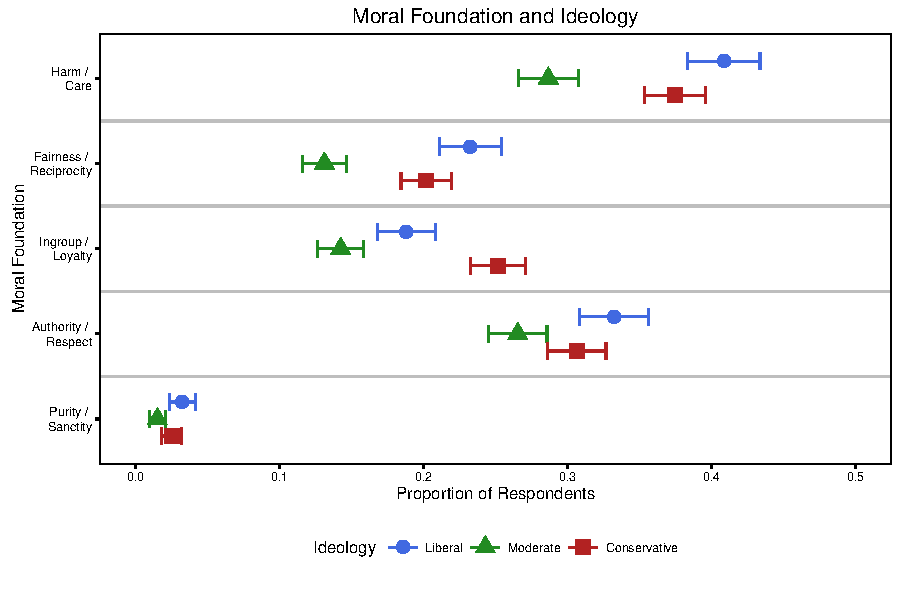
\includegraphics[scale=.9]{../calc/fig/fig1prop.pdf}
\caption{Weighted proportion of Respondents mentioning each of the moral foundations in any of their open-ended responses, along with 95\% confidence intervals. Additional plot including 2008 data is shown in the appendix, Figure~\ref{fig:appC1prop}}\label{fig:1prop}
\end{figure}

The patterns are largely consistent with theoretical expectations. Liberals were more likely than conservatives or moderates to mention the harm/care foundation. Almost half of the respondents identifying as liberals mentioned words belonging to the harm/care category in their responses. Furthermore, they were more likely than conservatives to mention the fairness/reciprocity foundation. This pattern is consistent with Moral Foundations Theory, as is the tendency for a greater proportion of conservatives to reference the ingroup/loyalty foundation than liberals or moderates. There were some notable contradictions, however. Fewer liberals used fairness/reciprocity words than authority/respect words. Indeed, the proportion of liberal respondents referencing authority/respect is almost identical to the proportion of conservatives mentioning authority/respect. This result is inconsistent with previous research by moral foundations scholars.

The fact that the purity/sanctity foundation was almost never mentioned by any of the respondents is surprising, since other studies found that the purity/sanctity foundation plays a very important role when looking at ideological differences \citep{koleva2012tracing}. This result suggests that subsequent analyses of survey responses might necessitate a revision of the moral foundation dictionary, since the terms contained in the dictionary might not be relevant for political evaluations. Accordingly, some of the words (e.g. in the case of purity/sanctity) are too uncommon in the political context. Due to the very rare mentioning of the purity/sanctity dimension, the subsequent analyses will concentrate on the remaining four moral foundations.

Overall, these results provide an inconclusive picture on the moral foundations of political reasoning. While most patterns are consistent with our theoretical expectations, the findings for the authority/respect dimension contradict Moral Foundations Theory.\footnote{Instead of looking at the aggregation of all survey items, we can also investigate the patterns in smaller subsets of responses (see Appendix~\ref{app:desc}). For example, taking into account only open-ended responses related to the evaluations of parties \textit{or} candidates shows the same basic patterns as in the pooled analysis. The appendix additionally presents the same results based on the 2008 ANES.}

In a subsequent step, I estimated logit models using ideology (and the control variables discussed above) to predict the individual probability of referring to each of the moral foundations (excluding purity/sanctity). Note that all models control for the total number of words used by each respondent for their open-ended responses.\footnote{The full logistic regression results for this and all subsequent models discussed the remainder of the paper are presented in Appendix~\ref{app:tables}}. Figure~\ref{fig:2ideol} displays the expected change in predicted probabilities of mentioning each moral foundation for liberals and conservatives holding all other variables constant at their respective means. Like the analyses in Figure~\ref{fig:2ideol}, the responses for each individual were collapsed such that the dependent variables indicate whether any of their responses contained a reference to the moral foundations as identified by the MF dictionary. 

\begin{figure}[h]\centering
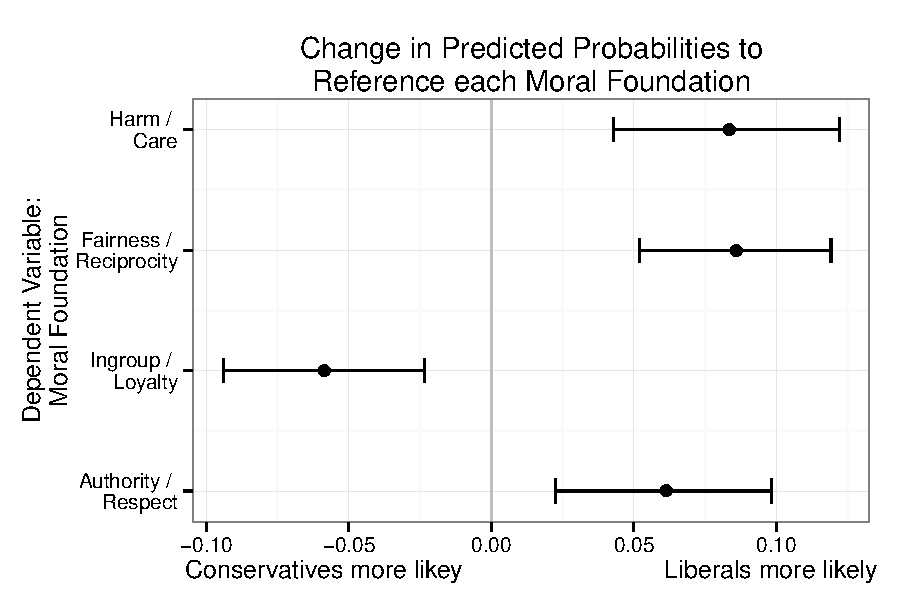
\includegraphics[scale=.9]{../calc/fig/fig2ideol.pdf}
\caption{Difference in predicted probabilities to reference each moral foundation between liberals and conservatives, holding all other control variables at their respective means (along with 95\% confidence intervals). Positive values indicate that liberals are more likely to reference the respective moral foundations than conservatives, and vice versa. Estimates are based on individual logit models for each foundation. Additional plot including 2008 data is shown in the appendix, Figure~\ref{fig:appD1ideol}, and full model results are displayed in Table~\ref{tab:m2ideol}.}\label{fig:2ideol}
\end{figure}

Positive values indicate a higher probability of mentioning the respective moral foundation in a response among respondents who identified as liberals, while negative values indicate a higher probability among conservatives. The effects are consistent with the first hypothesis for three out of four moral foundations. Liberals are significantly more likely to mention harm/care and fairness/reciprocity when evaluating political parties and candidates than liberals. The probability of mentioning a word connected to the harm/care foundation is about 7.5 percentage points higher among liberals than conservatives. The effect is of similar size for the fairness/reciprocity dimension. Conversely, being conservative increases the likelihood of mentioning words that belong to the category of ingroup/loyalty by about 5 percentage points. However, liberals are significantly more likely to reference the moral foundation of authority/respect when evaluating political actors. This result is inconsistent with previous evidence regarding the endorsement of this foundation by conservatives. 

I conducted auxiliary analyses to probe the robustness of the patterns in Figure~\ref{fig:1prop} and \ref{fig:2ideol} and especially to investigate alternative explanations for the inconsistent finding regarding the moral foundation of authority/respect (detailed results are included in Appendix~\ref{app:robust}). As a first step, I replicated the analyses using the 2008 ANES (see Figure~\ref{fig:appD1ideol}). Overall, there are fewer patterns that are consistent with Moral Foundations Theory in 2008 than in 2012. Indeed, the only difference between liberals and conservatives that is significant is the proportion of respondents referencing the ingroup/loyalty foundation. One explanation for the inconsistency across years is the fact that the open-ended responses were recorded in a more indirect manner in 2008. Many responses in 2008 consist of the interviewer's summaries of the responses in verbatim.\footnote{For example, a response in the 2008 ANES describing what the respondent likes about the Republican candidate is recorded as follows: ``his views more or less on politics, R feels he knows alot about the issues in politics
[sic]''. On the other hand, a response for the same question in the 2012 ANES was recorded as: ``I think he is honest; he couldn't do a worse job; he understands business; he understands the American people and he understands our foreign relations with Israel//He understands how much we need our military; not for war but for peace. You need to be strong to have peace//He believes in God, very important. He believes in family. He believes in dignity. the human spirit// [sic]''. While some responses in 2008 were of better quality than the example presented here, the overall proportion of summarized responses is higher than in the 2012 data. As such, the average response length is shorter in 2008 than in 2012 (c.f. Figure~\ref{fig:appB2num} in the appendix).} The sample size in 2008 also is much smaller, which explains the higher uncertainties around the estimated proportions.

Another explanation for the inconsistencies in Figures \ref{fig:1prop} and \ref{fig:2ideol} is the uni-dimensional conceptualization of ideology. Although most previous work in this area implicitly assumes a single ideological dimension, this may be too simplistic to describe systematic individual differences. Thus, I repeated the analyses using a two-dimensional conceptualization of ideology differentiating between a social as well as an economic dimension as proposed by \citet[see Figure~\ref{fig:appD2soceco}]{feldman2014understanding}. While providing a more detailed picture for the dimensions of harm/care (driven especially by the economic dimension), fairness/reciprocity (social dimension), and ingroup/loyalty (economic dimension), the results for authority/respect are similar to the first analysis.

The inconsistent results for the authority dimension might also be an artifact due to some peculiarity of the moral foundations dictionary. There might be signal words that are attributed to the authority/respect dimension and especially salient when talking about Barack Obama. For example, the moral foundations dictionary includes ``leader'' as a signal word for the authority/respect dimension. Thus, the inconsistent finding may be due to the fact that Obama is often considered as a ``good leader'' among his supporters. In order to examine this issue, I repeated the analyses after omitting ``leader'' from the moral foundations dictionary. The results do not change substantially (see Figure~\ref{fig:appD3lead} in the appendix).

More detailed analyses of the open-ended responses suggest that liberals were more likely to reference the authority dimension as a virtue (after dis-aggregating the moral dictionary by valence, see \url{www.moralfoundations.org}), when talking about positive aspects about parties and candidates, as well as when discussing their in-party candidate. It appears that the Democratic candidate (Barack Obama) was viewed favorably by supporters due to considerations related to the moral foundation of authority/respect (see Figure~\ref{fig:appD4toD6} in the appendix). This result is a first indication that the differences in moral reasoning between liberals and conservatives are contingent upon the respective political environment.

Taken together, the results indicate that there are important differences between liberals and conservatives in their reliance on different moral considerations when evaluating political parties and candidates. However, the patterns are not unequivocally consistent with the predictions of Moral Foundations Theory. The fact that some foundations showed contrary patterns, as well as the failure to replicate the findings across years suggests that the reliance on moral foundations might be more context-specific than previously theorized.


\subsubsection{Determinants of Moral Reasoning}

Having shown that liberals and conservatives differ with regard to the moral foundations they emphasize when evaluating political actors, I next investigate whether the reliance on moral considerations is a product of exposure to political discourse. I predict the probability of mentioning any moral foundation with a series of logit models in which political sophistication, political media exposure, and frequency of political discussions are the key independent variables. Figure~\ref{fig:3learn} depicts the respective predicted probabilities when each independent variable (knowledge, media exposure, discussion) is increased from its empirical minimum value to its empirical maximum value, holding all other variables (including the number of words in each individual response) constant at their means.\footnote{Results for the 2008 replication of this as well as all subsequent analyses discussed in the remainder of paper are displayed in Appendix~\ref{app:robust}.}

\begin{figure}[h]\centering
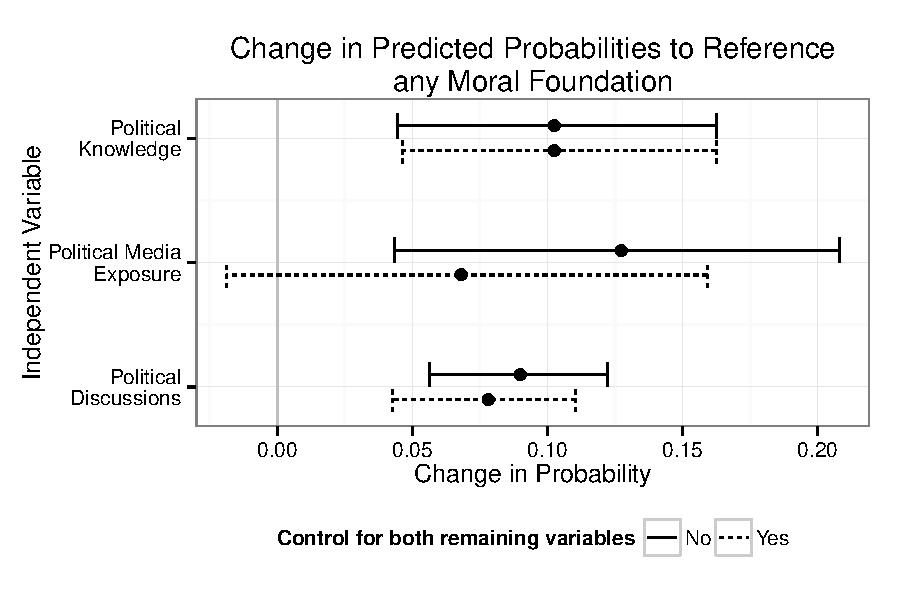
\includegraphics[scale=.9]{../calc/fig/fig3learn.pdf}
\caption{Change in predicted probabilities to reference any moral foundation depending on political knowledge, media exposure, and frequency of political discussions. The plot shows the difference in predicted probabilities if each of the independent variables is increased from its minimum to its maximum value holding all other variables constant at their respective means (along with 95\% confidence intervals). Positive values indicate higher probabilities of referencing any moral foundation. Estimates are based on logit models and dotted lines indicate estimates while controlling for both remaining variables. Additional plot including 2008 data is shown in the appendix, Figure~\ref{fig:appD7learn}, and full model results are displayed in Table~\ref{tab:m3learn}.}\label{fig:3learn}
\end{figure}

The results show that all three variables have a positive effect on the individual probability to make use of moral foundations when evaluating political parties and candidates. Higher political sophistication, higher exposure to political media and news, as well as more frequent political discussions increase the probability that individuals rely on moral considerations. Thus, citizens \textit{learn} to embed moral reasoning in their political evaluations. While moral intuitions themselves might well be innate, the extent to which individuals make use of these intuitions when thinking about politics and evaluating political actors may be more context-dependent and subject to individual heterogeneity.

The significant positive effect of frequent political discussions (even after controlling for the two remaining variables, political knowledge and media exposure), is especially interesting in this context. Citizens, who engage in frequent political arguments are more likely to use moral considerations when evaluating candidates and parties. This result suggests that morality serves as a rhetorical tool utilized to convince others of certain political views. Overall, positive relationships between political knowledge, media exposure, and political discussions and moral reasoning are quite robust, even controlling for individual response lengths.

In addition to examining the reference to moral foundations \textit{in general}, we can also consider whether the effects of political discourse increase the differences in the emphasis on specific dimensions between liberals and conservatives. Figure~\ref{fig:4ideolearn} presents the change in the effect of ideology on the probability to reference each of the moral foundations moderated by political knowledge, media exposure, and frequency of political discussions. Thus, each point in the figure displays the interaction effect between knowledge (or media exposure, or discussion) and ideology as a difference-in-difference in predicted probabilities holding all other variables constant at their respective means. For example, the positive effect for political knowledge on the probability to reference the harm/care foundation (top left part in the figure) indicates, that when political knowledge is increased from its empirical minimum to its maximum, the difference between liberals and conservatives is increased such that liberals are about 20 percentage points more likely to mention words belonging to the harm/care foundation than conservatives. In other words, positive effects imply that the gap between liberals and conservatives on the respective dimension is increased in favor of liberal respondents. Negative effects, on the other hand, indicate that the gap between liberals and conservatives is increased with conservatives becoming more likely to reference the respective moral dimension.

\begin{figure}[h]\centering
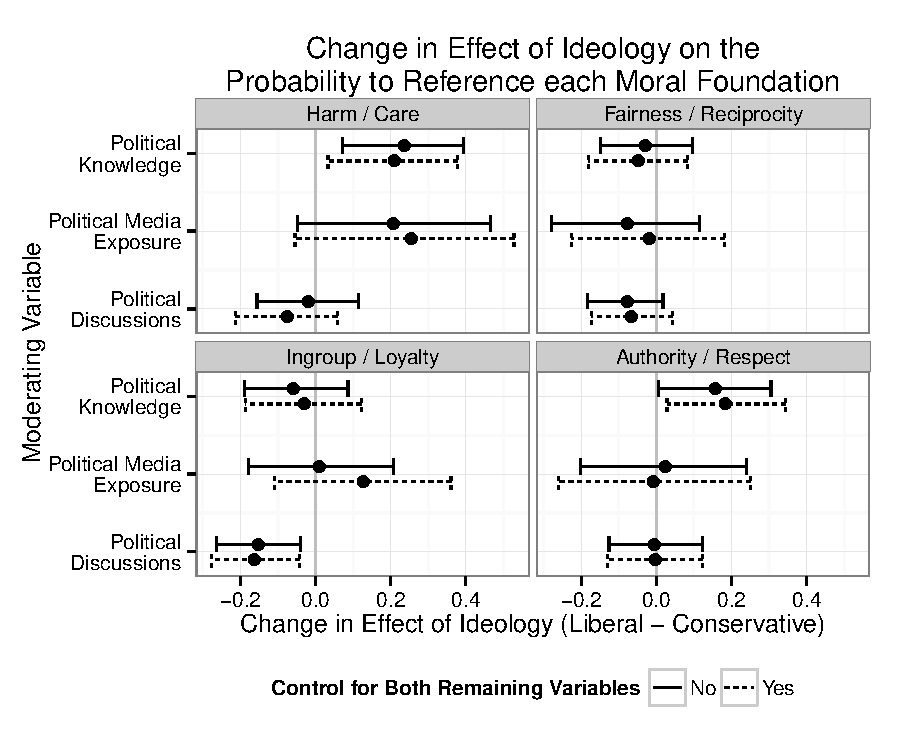
\includegraphics[scale=.9]{../calc/fig/fig4ideolearn.pdf}
\caption{Change in effect of ideology on predicted probabilities to reference each moral foundation moderated by political knowledge, media exposure, and frequency of political discussions (difference-in-difference). The plot shows how the difference in predicted probabilities to reference each moral foundation between liberals and conservatives changes if each of the independent variables is increased from its minimum to its maximum value holding all other variables constant at their respective means (along with 95\% confidence intervals). Positive values indicate that liberals are more likely to mention a specific moral foundation if they score high on the moderating variable (knowledge, exposure, or discussions), and vice versa. Estimates are based on individual logit models for each foundation and dotted lines indicate estimates while controlling for both remaining variables. Additional plot including 2008 data is shown in the appendix, Figure~\ref{fig:appD8ideolearn}, and full model results are displayed in Tables~\ref{tab:m4ideolearn2012a} to \ref{tab:m4ideolearn2008b}.}\label{fig:4ideolearn}
\end{figure}

In order to interpret these difference-in-difference effects, consider again the basic findings reported in Figure~\ref{fig:2ideol}. The estimates showed that on average, liberals were more likely to reference the foundations of harm/care, fairness/reciprocity, and authority/respect, whereas conservatives were more likely to mention considerations related to the ingroup/loyalty dimension. Turning to Figure~\ref{fig:4ideolearn}, we see that for individuals with high political knowledge and media exposure, the difference between liberals and conservatives in terms of the harm/care foundation was more pronounced: the difference between liberals and conservatives is increased such that liberals are even more likely to reference this dimension compared to conservatives. While we do not observe any meaningful moderation effects for the fairness/reciprocity dimension, there is some evidence that the ideological gap in the ingroup/loyalty dimension is higher for respondents who discuss politics more frequently, as well as in the authority/respect dimension for respondents with high political knowledge.

Overall, political knowledge, media exposure, and political discussions do not only affect general levels of moral reasoning but also moderate the ideological gap between liberals and conservatives. This finding indicates that the effects of political discourse cannot be reduced to an artifact of differences in political literacy and more elaborate argumentation. Some portion of the ideological differences in emphasis on moral foundations can therefore be described as a product of learning in the political environment.
\clearpage


\subsubsection{Consequences and Political Relevance of Moral Reasoning}

Previous research relying on the MFQ has linked moral foundations to an array of political outcomes, such as turnout \citep{johnson2014ideology}, candidate preferences \citep{iyer2010beyond}, and voting behavior \citep{franks2015using}. But do we see the same patterns for explicit moral reasoning as compared to latent moral foundations? As a first step, we will examine whether references to moral foundations affect political participation. Figure~\ref{fig:5turnout} displays the results of logit models predicting individual turnout as a function of individual references to moral foundations (as well as the regular set of control variables used in the previous analyses).

\begin{figure}[h]\centering
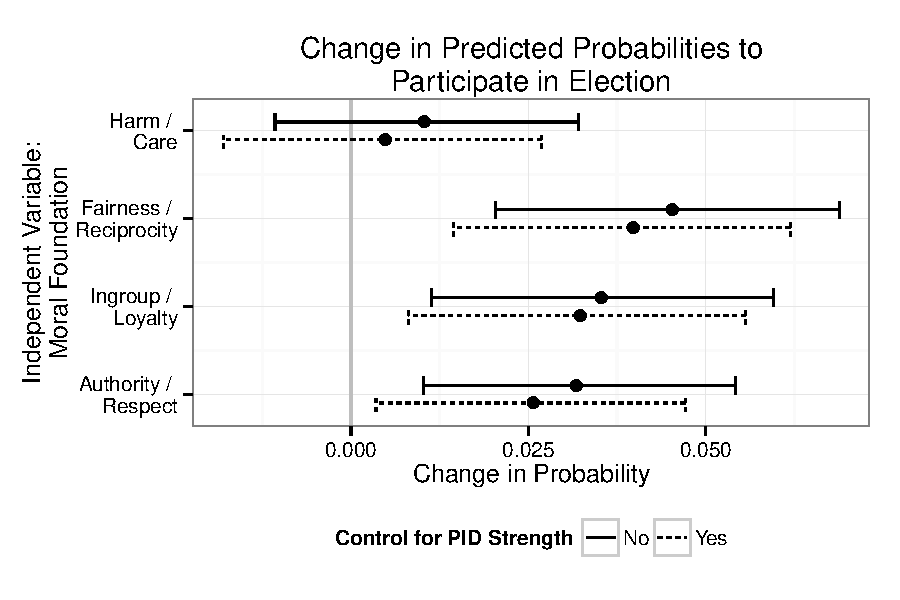
\includegraphics[scale=.9]{../calc/fig/fig5turnout.pdf}
\caption{Difference in predicted probabilities to participate in election between respondents who mentioned each moral foundation or not, holding all other control variables constant at their respective means (along with 95\% confidence intervals). Positive values indicate that respondents who mentioned the respective foundation are more likely to participate in the election, and vice versa. Estimates are based on a single logit model including dichotomous indicators for each foundation and dotted lines indicate estimates while additionally controlling for the strength of party identification. Additional plot including 2008 data is shown in the appendix, Figure~\ref{fig:appD9turnout}, and full model results are displayed in Table~\ref{tab:m5turnout}.}\label{fig:5turnout}
\end{figure}

Each of the moral foundations have a positive effect on the predicted probabilities of participating in the election (with the exception that the effect of harm/care is not statistically significant). For example, if a respondent mentions considerations related to fairness/reciprocity when discussing his or her political preferences, the probability of turning out to vote is increased by almost 5 percentage points, holding all other variables constant at their respective means. Note that the estimates are based on models that already take into account the length of individual responses. Furthermore, most of the effects stay significant and are only reduced marginally after controlling for the strength of individual party identification.

\begin{figure}[h]\centering
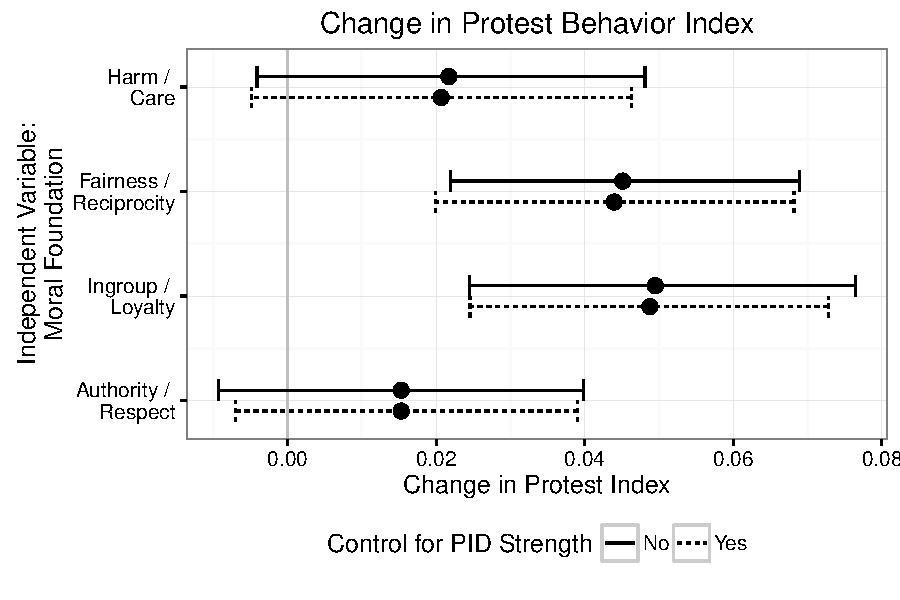
\includegraphics[scale=.9]{../calc/fig/fig6part.pdf}
\caption{Difference in predicted protest behavior index between respondents who mentioned each moral foundation or not, holding all other control variables constant at their respective means (along with 95\% confidence intervals). Positive values indicate that respondents who mentioned the respective foundation scored higher on an additive protest behavior index ranging from 0 to 3, and vice versa. Estimates are based on a single OLS model (using robust standard errors) including dichotomous indicators for each foundation and dotted lines indicate estimates while additionally controlling for the strength of party identification. Additional plot including 2008 data is shown in the appendix, Figure~\ref{fig:appD10part}, and full model results are displayed in Table~\ref{tab:m6part}.}\label{fig:6part}
\end{figure}

The influence of moral reasoning extends to other forms of participation. Figure~\ref{fig:6part} displays estimates from a linear regression predicting protest behavior (participation in demonstration, displaying signs or campaign stickers, signing petitions) based on moral foundations. Again, references to moral foundations generally has positive effects on political engagement outside of the ballot box. Consider the effect of ingroup/loyalty as an example. If respondents mentioned considerations related to this moral foundation, their additive protest index (ranging from 0 to 3) is increased by 0.1 points. This effect might not seem large, but bear in mind that the independent variable consists of a dichotomous indicator for references to any moral foundation in a set of open-ended questions. The fact that we can recover consistent and statistically significant effects on political participation in such a context (even after controlling for strength of party identification and the length of individual responses) is therefore quite meaningful.

Overall then, the analyses indicate that moral reasoning is positively associated with political engagement. That said, the analyses presented here are not sufficient to make a strong causal claim about the direction of this relationship. Yet, the results suggest that moral reasoning (as measured by open-ended survey responses) is powerfully related to different forms of political participation and engagement.

\begin{figure}[h]\centering
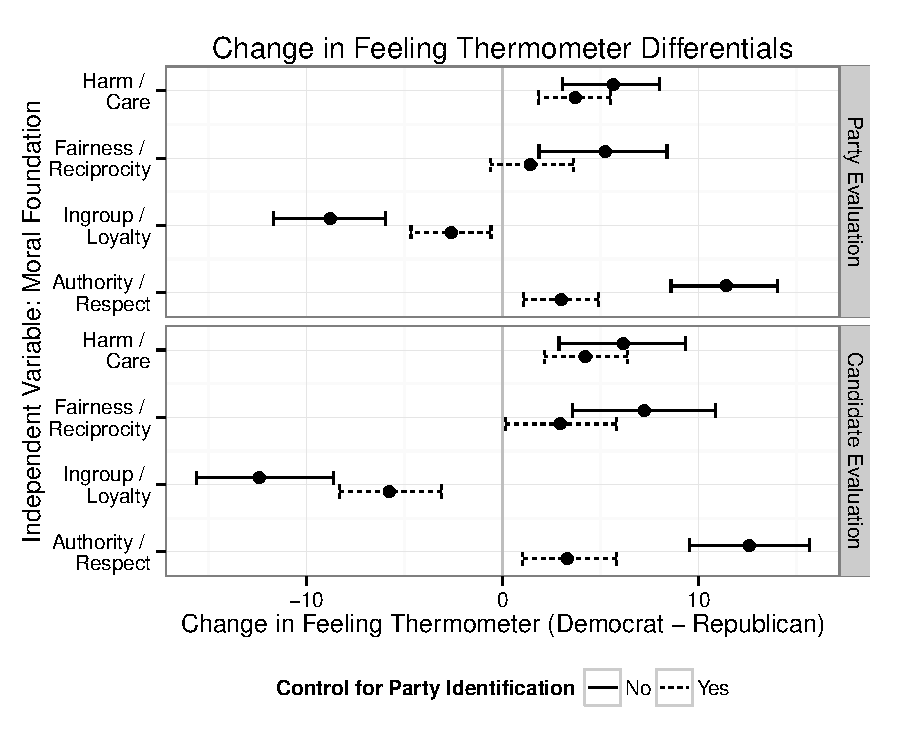
\includegraphics[scale=.9]{../calc/fig/fig7feel.pdf}
\caption{Change in predicted feeling thermometer differential between respondents who mentioned each moral foundation or not, holding all other control variables constant at their respective means (along with 95\% confidence intervals). Positive values indicate that respondents who mentioned the respective foundation evaluated the Democratic candidate/party more favorably than the Republican candidate/party, and vice versa. Estimates are based on a single OLS model (using robust standard errors) including dichotomous indicators for each foundation and dotted lines indicate estimates while additionally controlling for party identification. Additional plot including 2008 data is shown in the appendix, Figure~\ref{fig:appD11feel}, and full model results are displayed in Table~\ref{tab:m7feel}.}\label{fig:7feel}
\end{figure}

In the next step, we turn to the relationship of moral reasoning and political preferences themselves. Figure~\ref{fig:7feel} presents the results of linear regressions of moral foundations predicting the change in the feeling thermometer differential between the Republican and the Democratic Presidential candidate (top part of the figure) and the change in the feeling thermometer differential between the Republican and Democratic party. Positive values indicate more favorable evaluations for the Democratic candidate or party and negative values indicate more favorable evaluations of the Republican candidate or party. The patterns are largely consistent with the previous results on ideological differences. Individuals who mention considerations related to harm/care, fairness/reciprocity, and authority/respect evaluate the Democratic candidates on average 5 points higher than the Republican candidates (on a 100 point scale). On the other hand, if individuals emphasized the ingroup/loyalty dimension, they reported stronger preferences for the Republican candidates. These effects are robust after controlling for individual party identification. Thus, in both analyses in Figure~\ref{fig:7feel}, we observed sizable and significant effects for the influence of moral reasoning. This result is especially noteworthy given that respondents were not explicitly asked about morality. Furthermore, it is not necessary to distinguish between responses for either party or between positive and negative statements in order to recover meaningful patterns. Even though we are simply looking at moral reasoning in the collection of all positive and negative statements about both candidates and parties, we observe consistent and substantial effects on subsequent evaluations. The moral considerations evoked by respondents allow us to make inferences about their political attitudes and behavior irrespective of the specific party or candidate they are evaluating.

Lastly, Figure~\ref{fig:8vote} finally presents the changes in expected probabilities of voting for the Democratic (vs. the Republican) presidential candidate in the 2012 election for individuals mentioning the moral foundations in their open-ended responses. The estimated probabilities are based on logit models including dummies for each moral foundation as independent variables as well as several sociodemographic control variables, which were held constant at their mean values when calculating expected values.

\begin{figure}[h]\centering
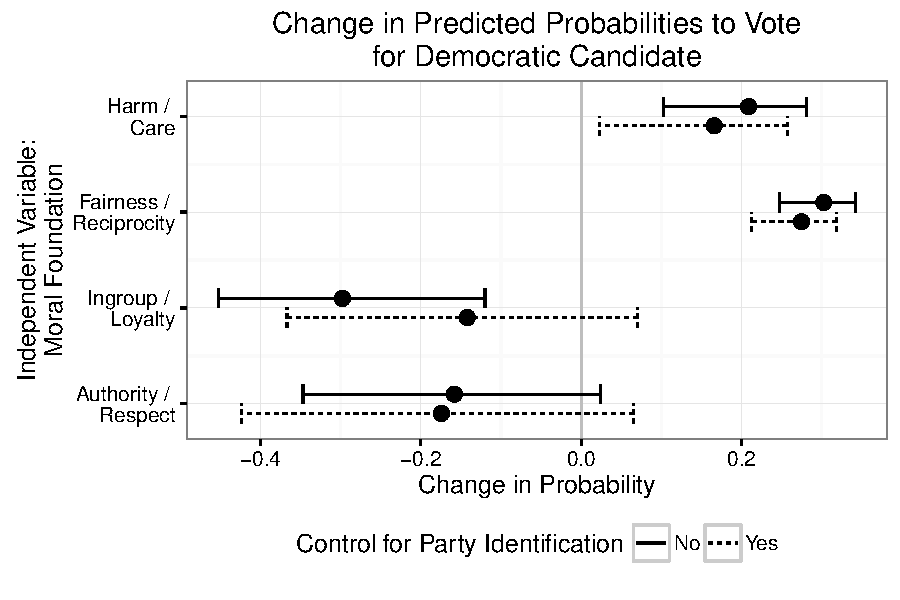
\includegraphics[scale=.9]{../calc/fig/fig8vote.pdf}
\caption{Difference in predicted probabilities to vote for Democratic candidate between respondents who mentioned each moral foundation or not, holding all other control variables constant at their respective means (along with 95\% confidence intervals). Positive values indicate that respondents who mentioned the respective foundation are more likely to vote for the Democratic candidate, and vice versa. Estimates are based on a single logit model including dichotomous indicators for each foundation and dotted lines indicate estimates while additionally controlling for party identification. Additional plot including 2008 data is shown in the appendix, Figure~\ref{fig:appD12vote}, and full model results are displayed in Table~\ref{tab:m8vote}.}\label{fig:8vote}
\end{figure}

Again, the patterns are strikingly similar to the results presented thus far. Individuals who mentioned moral considerations related to the harm/care foundation are (slightly) more likely to vote for the Democratic candidate. The effect for the fairness/reciprocity foundation is also positive: respondents who mentioned this foundation were more likely to vote for Barack Obama than for Mitt Romney. Respondents who emphasized the ingroup/loyalty foundation, on the other hand, were less likely to vote for the Democratic candidate. While these results appear to be relatively consistent with Moral Foundations Theory, we see again that the effect for the authority/respect foundation deviates from our expectations: respondents mentioning this foundation were more likely to vote for the Democratic candidate. Overall, Figure~\ref{fig:8vote} shows that it is possible to predict voting behavior simply by observing the moral dimensions of the respondents' political reasoning, without taking into account which candidate they described, and whether the description is framed positively or negatively. Moreover, these effects persist after controlling for individual party identification.


\section{Conclusion}

The goal of this paper was to investigate whether the ideological differences in the emphasis of moral foundations manifests itself in individual reasoning about political actors. The analyses of open-ended survey responses can provide important insights beyond previous research because it allows us to evaluate whether citizens make references to moral considerations in a political context that does not induce an explicit connection to morality. In contrast to previous accounts of Moral Foundations theory, I argue that the reliance on moral reasoning as such is moderated by political knowledge, media exposure, and political discussions. The emphasis of specific moral foundations, in turn, was expected to influence important political outcomes such as participation, candidate evaluations, and voting behavior.

The empirical evidence discussed in this paper is only partly consistent with previous research on moral foundations and ideology. The first hypothesis, which predicted systematic patterns in the emphasis on moral considerations among liberals and conservatives, was supported for three out of four foundations. Liberals are more likely to mention considerations related to harm/care and fairness/reciprocity when discussing their political preferences, whereas conservatives are more likely to emphasize the moral foundation of ingroup/loyalty.

According to the second hypothesis, it was expected that individuals show heterogeneity in terms of their tendency to rely on moral reasoning. The results indicated that political knowledge, discussions, as well as media consumption increase the reliance on moral considerations. Thus, the evidence suggests that moral reasoning is part of a broader political learning process. At least in some cases, this learning process appears to imply an increased differentiation between liberals and conservatives in terms of the focus on specific foundations as described by Moral Foundations Theory.

The last part of the analyses focused on the political relevance of moral reasoning as conceptualized by open-ended survey responses. The results here revealed consistent relationships between individual moral foundations and different forms of political participation, candidate evaluation, and voting behavior. As such, moral reasoning measured using open-ended survey responses is a politically meaningful and influential concept.

The contributions of this paper are therefore twofold. This study adds to the existing literature on moral foundations by providing new insights into the mechanisms underlying its relationship with ideology. From a general methodological perspective, the paper emphasizes the potential benefits of incorporating open-ended survey responses in research focusing on the determinants and structure of ideology and political reasoning. The paper shows that one can directly assess moral reasoning in surveys that do not contain the MFQ or related measures, simply by relying on open-ended survey responses.

However, it should be noted that many of the relationships discussed in the paper could not be recovered in a replication using data from the 2008 ANES. While the basic patterns persist, many effects in 2008 fail to reach statistical significance. This issue can partly be explained by the fact that the open-ended responses in 2008 were recorded by some interviewers as indirect summaries rather than direct verbatim responses. As such, the open-ended survey data for 2012 is better suited to identify moral references through the respondent's open-ended responses.

The results presented here provide several directions for future research. The fact that purity/sanctity was almost never mentioned as well as the inconsistent effect of ideology on the authority/respect dimension can be attributed to the fact that the moral foundations dictionary was originally used for the analyses of sermons. Accordingly, subsequent analyses could revise the dictionary in order to make it more applicable for the analyses of survey responses. An alternative approach to the analysis of open-ended survey responses could be the implementation of structural topic models as described by \citet{roberts2014structural}: instead of using explicit word lists to identify moral reasoning, it would possible to identify specific topics in open-ended responses that are consistent with the moral foundations described by \citet{haidt2008moral} \citep[see also][]{lin2008joint}.

One important issue that remains unresolved is the question of causality. \citet{graham2009liberals} rightfully stated that the causal nature of the relationship between moral foundations and ideology is not yet established. Their study did not settle whether individuals first identify as liberal or conservative and then adapt their respective moral judgments, or whether moral considerations shape and structure subsequent ideological thinking itself. Recent research focusing on elite influences on moral reasoning suggests that elite rhetoric plays an important role in shaping individual moral judgment \citep[see for example][]{clifford2013words,clifford2015concerns}. However, directly examining the underlying causal mechanism requires additional research where moral reasoning is manipulated experimentally.

It would also be worth investigating whether the patterns regarding moral reasoning change over larger periods of time using this method in order to further establish the context-specific nature of moral reasoning. At this time, however, full-text open-ended survey responses are not available in the ANES prior to 2008.

Overall, the analyses of open-ended survey responses can provide important and valuable insights in the context of moral foundations and the individual underpinnings of political ideology. Utilizing available responses to open-ended survey questions provides a useful and still largely neglected data source to investigate political reasoning.


\clearpage
\bibliographystyle{/data/Copy/1-src/lit/apsr2006}
\bibliography{/data/Copy/1-src/lit/Literature}

\clearpage
\flushleft\footnotesize\singlespacing
\appendices
\appendixpage
\renewcommand\thesubsection{\Roman{subsection}}
Kraft, Patrick W. 2016.\\``Moral Foundations of Political Reasoning. Investigating the Moral Underpinnings of Political Judgment.''

\startcontents[sections]
\printcontents[sections]{l}{1}{\setcounter{tocdepth}{2}}
\clearpage

\section{Moral Foundations Dictionary}\label{app:dict}
\renewcommand\thefigure{\thesection.\arabic{figure}}
\renewcommand\thetable{\thesection.\arabic{table}}
\setcounter{figure}{0}
\setcounter{table}{0}

\textit{Sources:}\\
\citet{graham2009liberals}, as well as \url{http://www.moralfoundations.org/}
\vspace{.5cm}

\textit{Note:}\\
Words with (*) indicate that the word stem rather than the exact word was matched in the open-ended survey responses.
\vspace{.5cm}

\textbf{Harm:}\\
safe*, peace*, compassion*, empath*, sympath*, care, caring, protect*, shield, shelter, amity, secur*, benefit*, defen*, guard*, preserve, harm*, suffer*, war, wars, warl*, warring, fight*, violen*, hurt*, kill, kills, killer*, killed, killing, endanger*, cruel*, brutal*, abuse*, damag*, ruin*, ravage, detriment*, crush*, attack*, annihilate*, destroy, stomp, abandon*, spurn, impair, exploit, exploits, exploited, exploiting, wound*
\vspace{.5cm}

\textbf{Fairness:}\\
fair, fairly, fairness, fair*, fairmind*, fairplay, equal*, justice, justness, justifi*, reciproc*, impartial*, egalitar*, rights, equity, evenness, equivalent, unbias*, tolerant, equable, balance*, homologous, unprejudice*, reasonable, constant, honest*, unfair*, unequal*, bias*, unjust*, injust*, bigot*, discriminat*, disproportion*, inequitable, prejud*, dishonest, unscrupulous, dissociate, preference, favoritism, segregat*, exclusion, exclud*
\vspace{.5cm}

\textbf{Ingroup:}\\
together, nation*, homeland*, family, families, familial, group, loyal*, patriot*, communal, commune*, communit*, communis*, comrad*, cadre, collectiv*, joint, unison, unite*, fellow*, guild, solidarity, devot*, member, cliqu*, cohort, ally, insider, foreign*, enem*, betray*, treason*, traitor*, treacher*, disloyal*, individual*, apostasy, apostate, deserted, deserter*, deserting, deceiv*, jilt*, imposter, miscreant, spy, sequester, renegade, terroris*, immigra*
\vspace{.5cm}

\textbf{Authority:}\\
obey*, obedien*, duty, law, lawful*, legal*, duti*, honor*, respect, respectful*, respected, respects, order*, father*, mother, motherl*, mothering, mothers, tradition*, hierarch*, authorit*, permit, permission, status*, rank*, leader*, class, bourgeoisie, caste*, position, complian*, command, supremacy, control, submi*, allegian*, serve, abide, defere*, defer, revere*, venerat*, comply, defian*, rebel*, dissent*, subver*, disrespect*, disobe*, sediti*, agitat*, insubordinat*, illegal*, lawless*, insurgent, mutinous, defy*, dissident, unfaithful, alienate, defector, heretic*, nonconformist, oppose, protest, refuse, denounce, remonstrate, riot*, obstruct
\vspace{.5cm}

\textbf{Purity:}\\
piety, pious, purity, pure*, clean*, steril*, sacred*, chast*, holy, holiness, saint*, wholesome*, celiba*, abstention, virgin, virgins, virginity, virginal, austerity, integrity, modesty, abstinen*, abstemiousness, upright, limpid, unadulterated, maiden, virtuous, refined, intemperate, decen*, immaculate, innocent, pristine, humble, disgust*, deprav*, disease*, unclean*, contagio*, indecen*, sin, sinful*, sinner*, sins, sinned, sinning, slut*, whore, dirt*, impiety, impious, profan*, gross, repuls*, sick*, promiscu*, lewd*, adulter*, debauche*, defile*, tramp, prostitut*, unchaste, wanton, profligate, filth*, trashy, obscen*, lax, taint*, stain*, tarnish*, debase*, desecrat*, wicked*, blemish, exploitat*, pervert, wretched*
\vspace{.5cm}

%\textbf{General:}\\
%righteous*, moral*, ethic*, value*, upstanding, good, goodness, principle*, blameless, exemplary, lesson, canon, doctrine, noble, worth*, ideal*, praiseworthy, commendable, character, proper, laudable, correct, wrong*, evil, immoral*, bad, offend*, offensive*, transgress*, honest*, lawful*, legal*, piety, pious, wholesome*, integrity, upright, decen*, indecen*, wicked*, wretched*


\clearpage
\section{Overview Open-Ended Responses}\label{app:oview}
\renewcommand\thefigure{\thesection.\arabic{figure}}
\renewcommand\thetable{\thesection.\arabic{table}}
\setcounter{figure}{0}
\setcounter{table}{0}

% latex table generated in R 3.2.3 by xtable 1.7-4 package
% Tue Jan 19 19:37:46 2016
\begin{table}[ht]
\centering
\begin{tabular}{lcc}
  \hline
 & N & Percent \\ 
  \hline
Spanish Interview (2008) & 94 & 4.05 \\ 
  Spanish Interview (2012) & 228 & 3.86 \\ 
  No Responses (Overall, 2008) & 158 & 7.09 \\ 
  No Responses (Overall, 2012) & 392 & 6.89 \\ 
  No Responses (Candidate Evaluations, 2008) & 328 & 14.13 \\ 
  No Responses (Candidate Evaluations, 2012) & 761 & 12.87 \\ 
  No Responses (Party Evaluations, 2008) & 584 & 25.15 \\ 
  No Responses (Party Evaluations, 2012) & 1503 & 25.41 \\ 
   \hline
\end{tabular}
\caption{Missing open-ended responses} 
\label{tab:appB1mis}
\end{table}


\begin{figure}[h]\centering
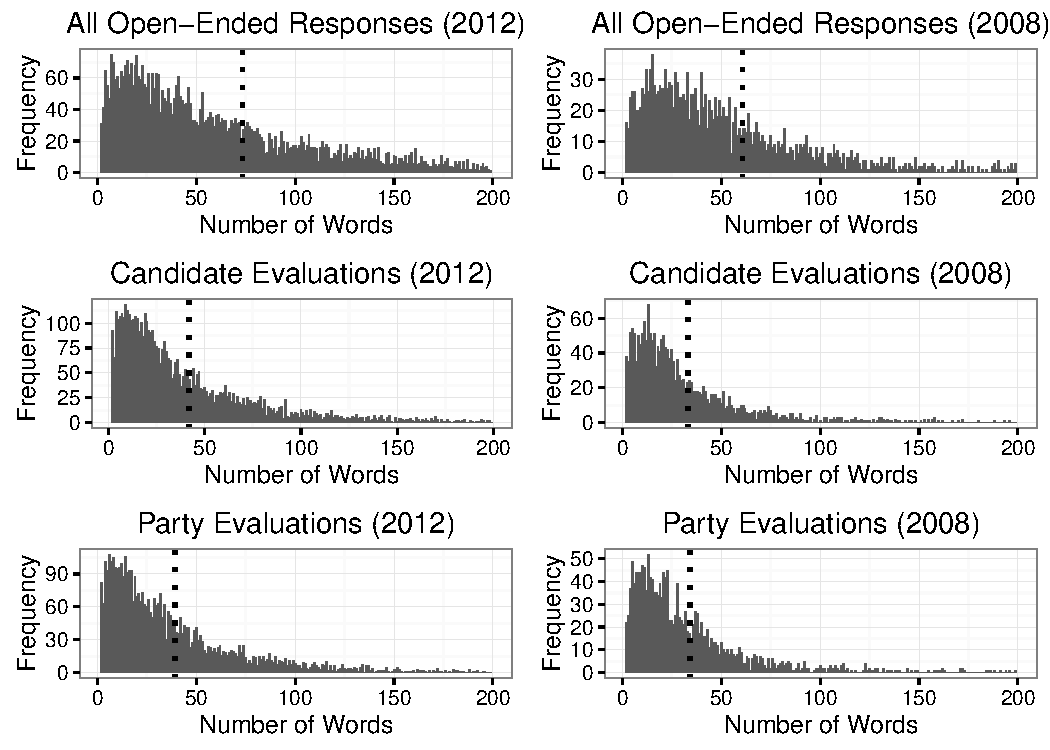
\includegraphics[scale=.7]{../calc/fig/appB2num.pdf}
\caption{Histograms displaying the distribution of individual response lengths in number of words for each respective item category. Dotted lines indicate the average response length.}\label{fig:appB2num}
\end{figure}

\clearpage
\section{Additional Descriptive Plots}\label{app:desc}
\renewcommand\thefigure{\thesection.\arabic{figure}}
\renewcommand\thetable{\thesection.\arabic{table}}
\setcounter{figure}{0}
\setcounter{table}{0}

\begin{figure}[h]
  \centering
  \caption{Weighted proportion of Respondents mentioning each of the moral foundations in any of their open-ended responses, along with 95\% confidence intervals.}
  \begin{subfigure}[t]{0.49\textwidth}
    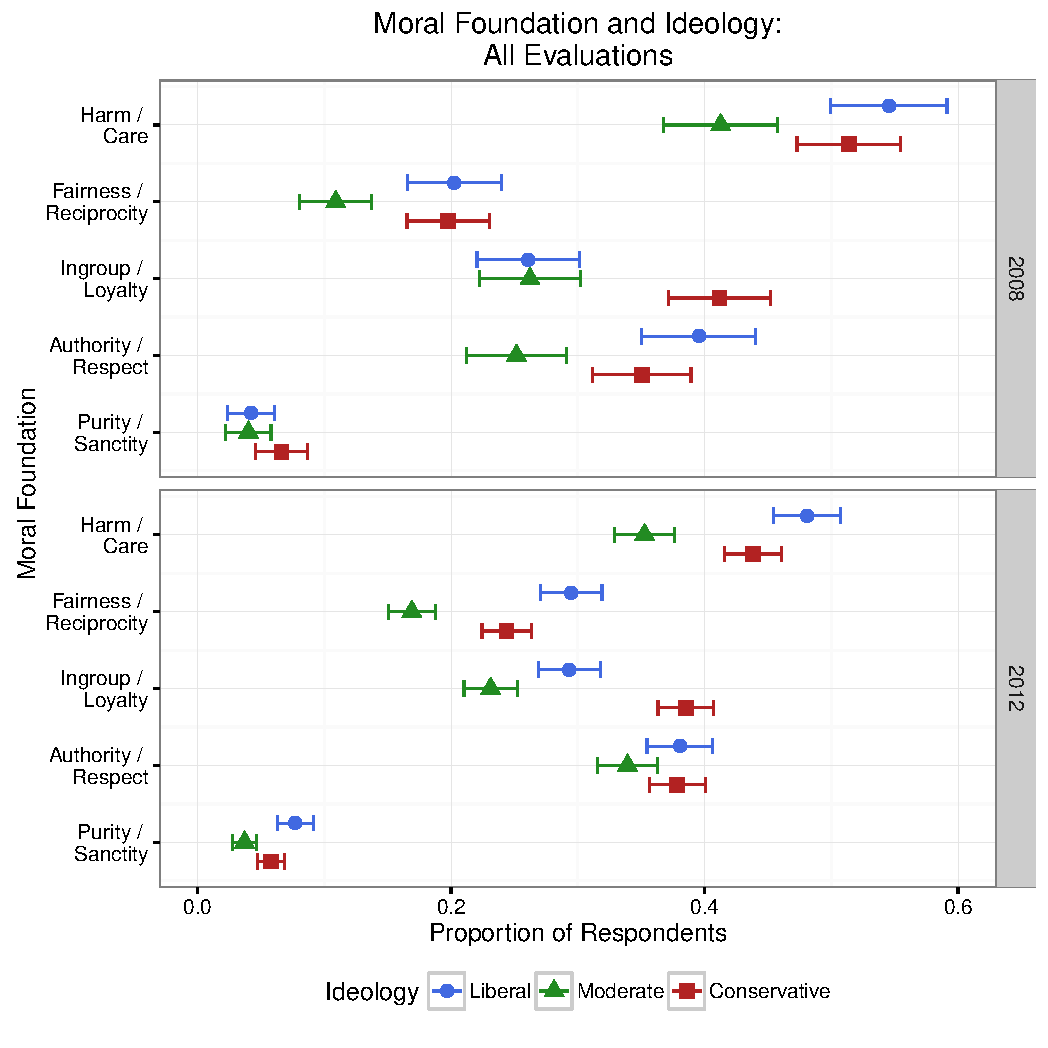
\includegraphics[scale=.4]{../calc/fig/appC1prop.pdf}
\caption{Proportions based on all open-ended responses}\label{fig:appC1prop}
  \end{subfigure}
  \begin{subfigure}[t]{0.49\textwidth}
    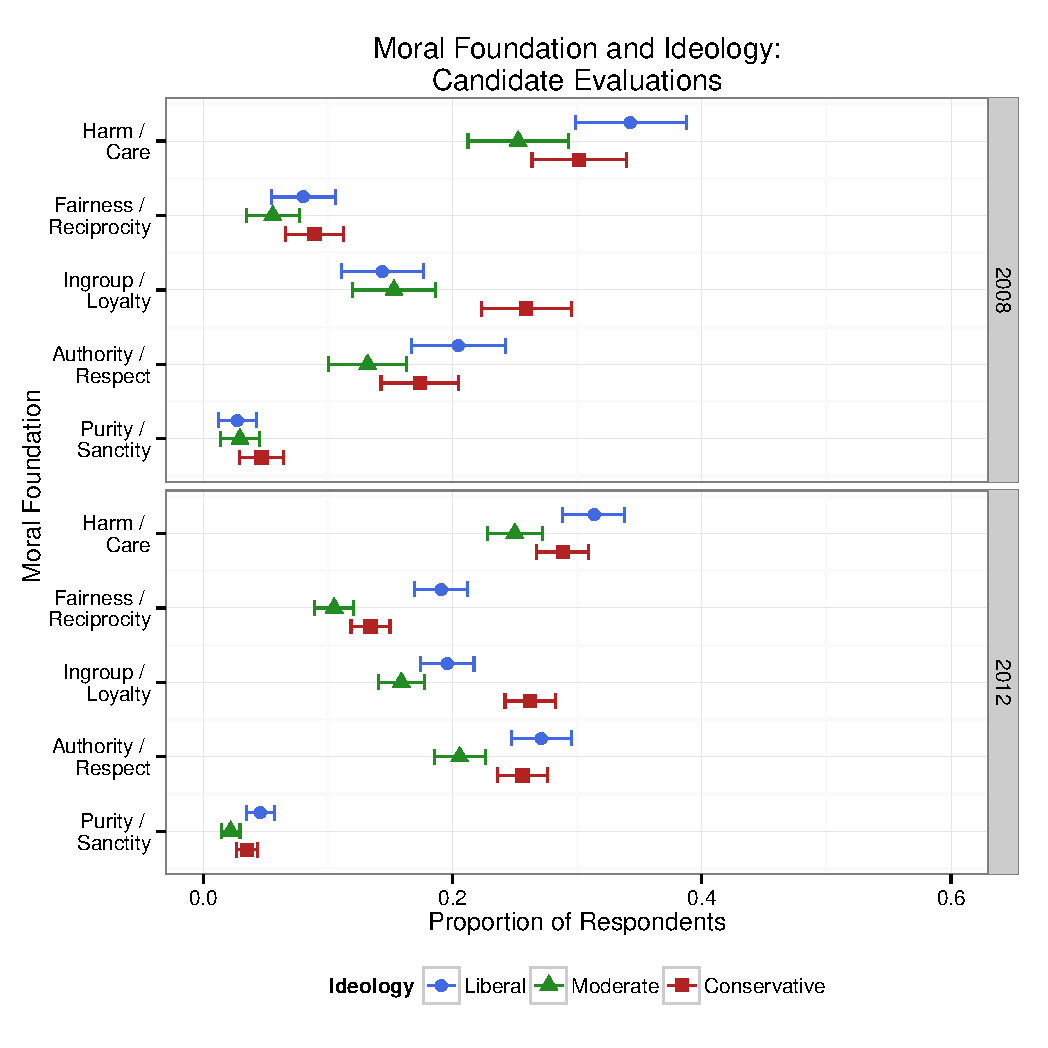
\includegraphics[scale=.4]{../calc/fig/appC2cand.pdf}
\caption{Proportions based on candidate evaluations}\label{fig:appC2cand}
  \end{subfigure}
  \begin{subfigure}[t]{0.49\textwidth}
    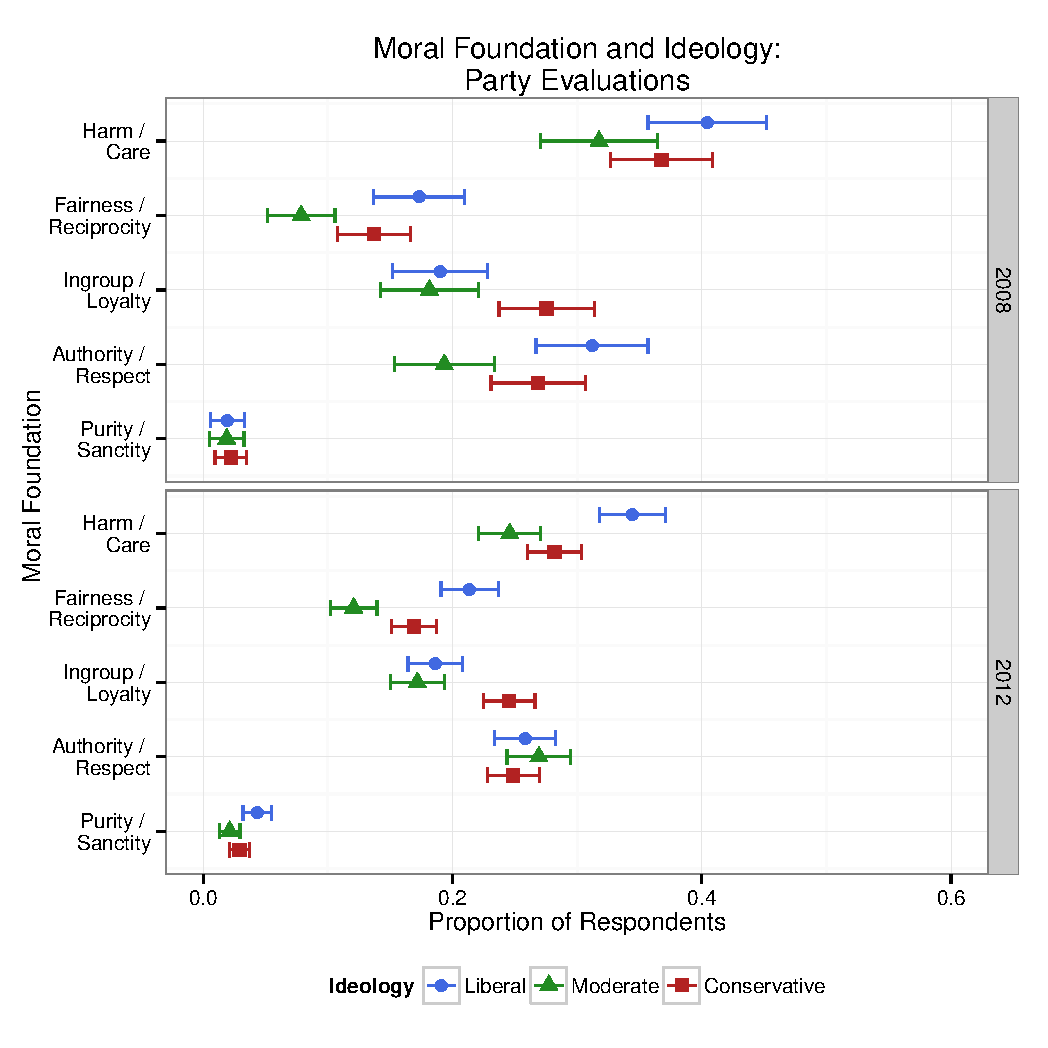
\includegraphics[scale=.4]{../calc/fig/appC3party.pdf}
\caption{Proportions based on party evaluations}\label{fig:appC3party}
  \end{subfigure}
\end{figure}


\clearpage
\section{Alternative Model Specifications and Robustness Checks}\label{app:robust}
\renewcommand\thefigure{\thesection.\arabic{figure}}
\renewcommand\thetable{\thesection.\arabic{table}}
\setcounter{figure}{0}
\setcounter{table}{0}


\subsection{Ideological differences in moral reasoning including 2008 ANES data}

\begin{figure}[h]
  \centering
  \caption{Difference in predicted probabilities to reference each moral foundation between liberals and conservatives, holding all other control variables at their respective means (along with 95\% confidence intervals). Positive values indicate that liberals are more likely to reference the respective moral foundations than conservatives, and vice versa. Estimates are based on individual logit models for each foundation.}
  \begin{subfigure}[t]{0.49\textwidth}
    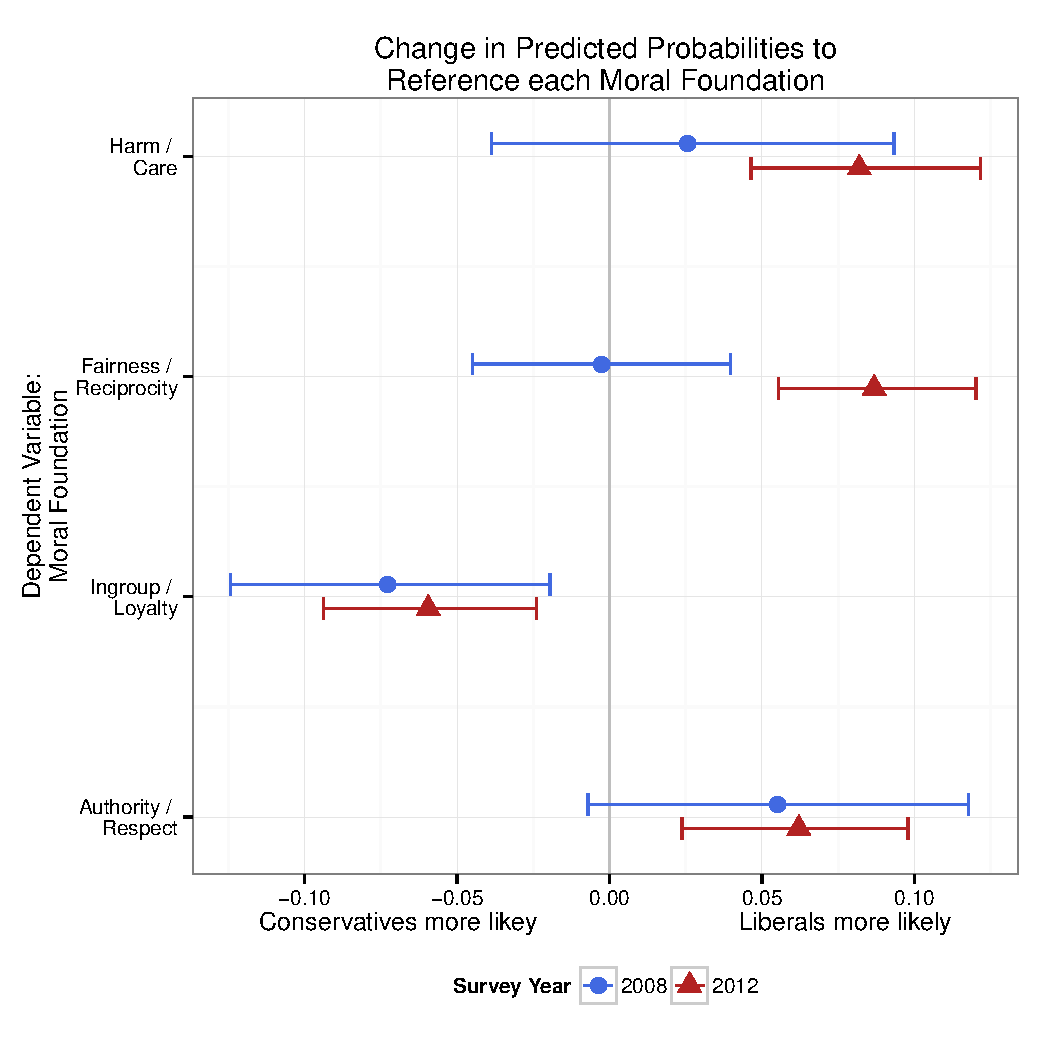
\includegraphics[scale=.4]{../calc/fig/appD1ideol.pdf}
    \caption{Basic models including data from 2008 ANES. Full model results are reported in Table \ref{tab:m2ideol}.}\label{fig:appD1ideol}
  \end{subfigure}
  \begin{subfigure}[t]{0.49\textwidth}
    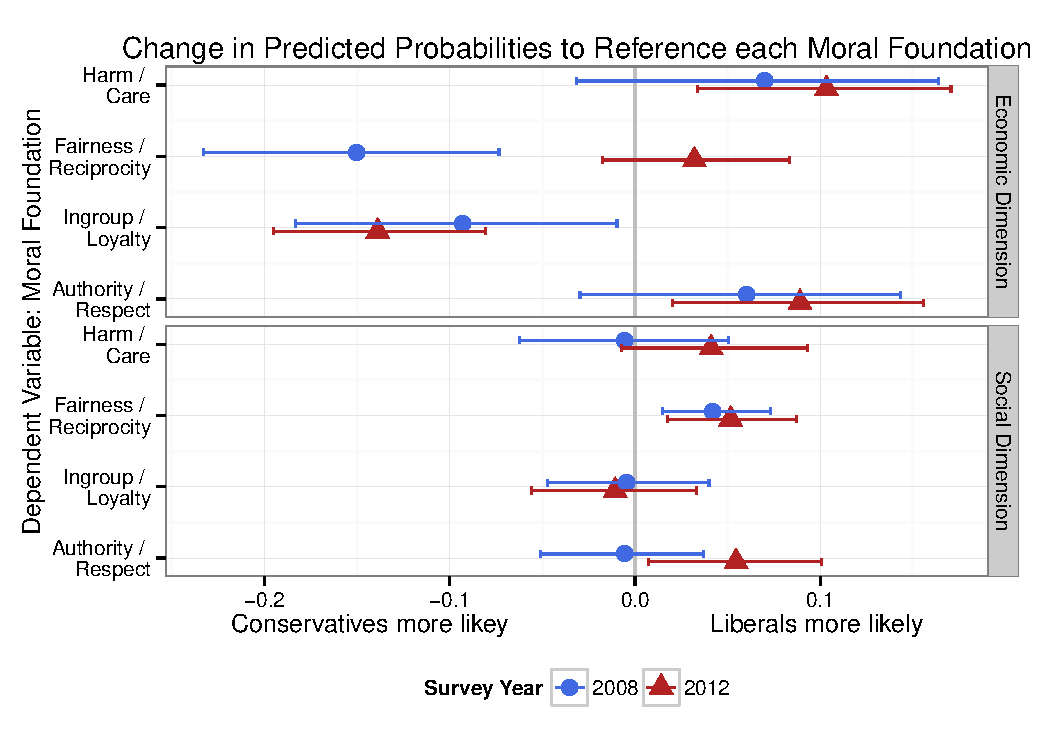
\includegraphics[scale=.4]{../calc/fig/appD2soceco.pdf}
    \caption{Models differentiating between economic and social dimension of ideology. Full model results are reported in Table \ref{tab:m2soceco}.}\label{fig:appD2soceco}
  \end{subfigure}
  \begin{subfigure}[t]{0.49\textwidth}
    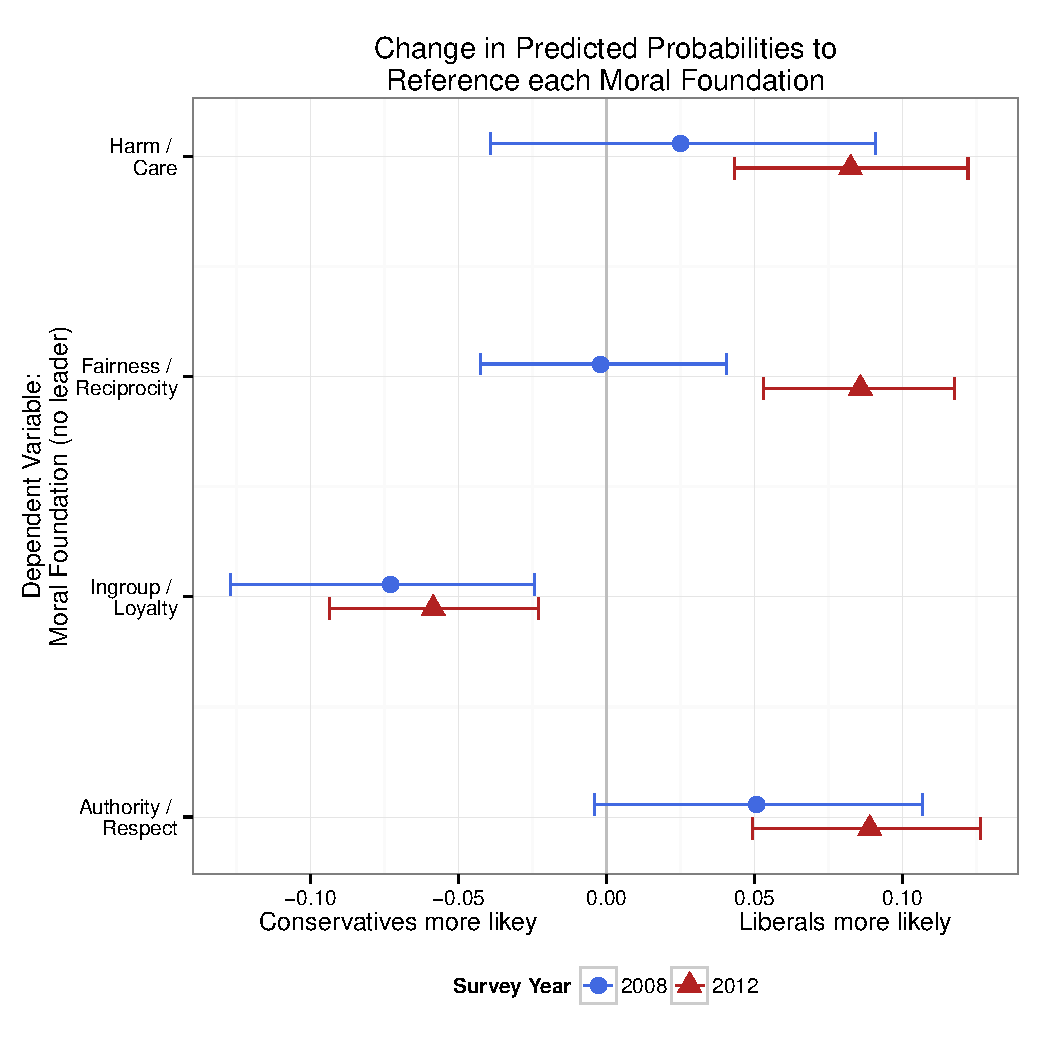
\includegraphics[scale=.4]{../calc/fig/appD3lead.pdf}
    \caption{Models omitting ``leader'' from the moral dictionary. Full model results are reported in Table \ref{tab:m2lead}.}\label{fig:appD3lead}
  \end{subfigure}
\end{figure}

\begin{figure}[h]
  \centering
  \caption{Difference in predicted probabilities to reference each moral foundation between liberals and conservatives, holding all other control variables at their respective means (along with 95\% confidence intervals). Positive values indicate that liberals are more likely to reference the respective moral foundations than conservatives, and vice versa. Estimates are based on individual logit models for each foundation.}\label{fig:appD4toD6}
  \begin{subfigure}[t]{0.49\textwidth}
    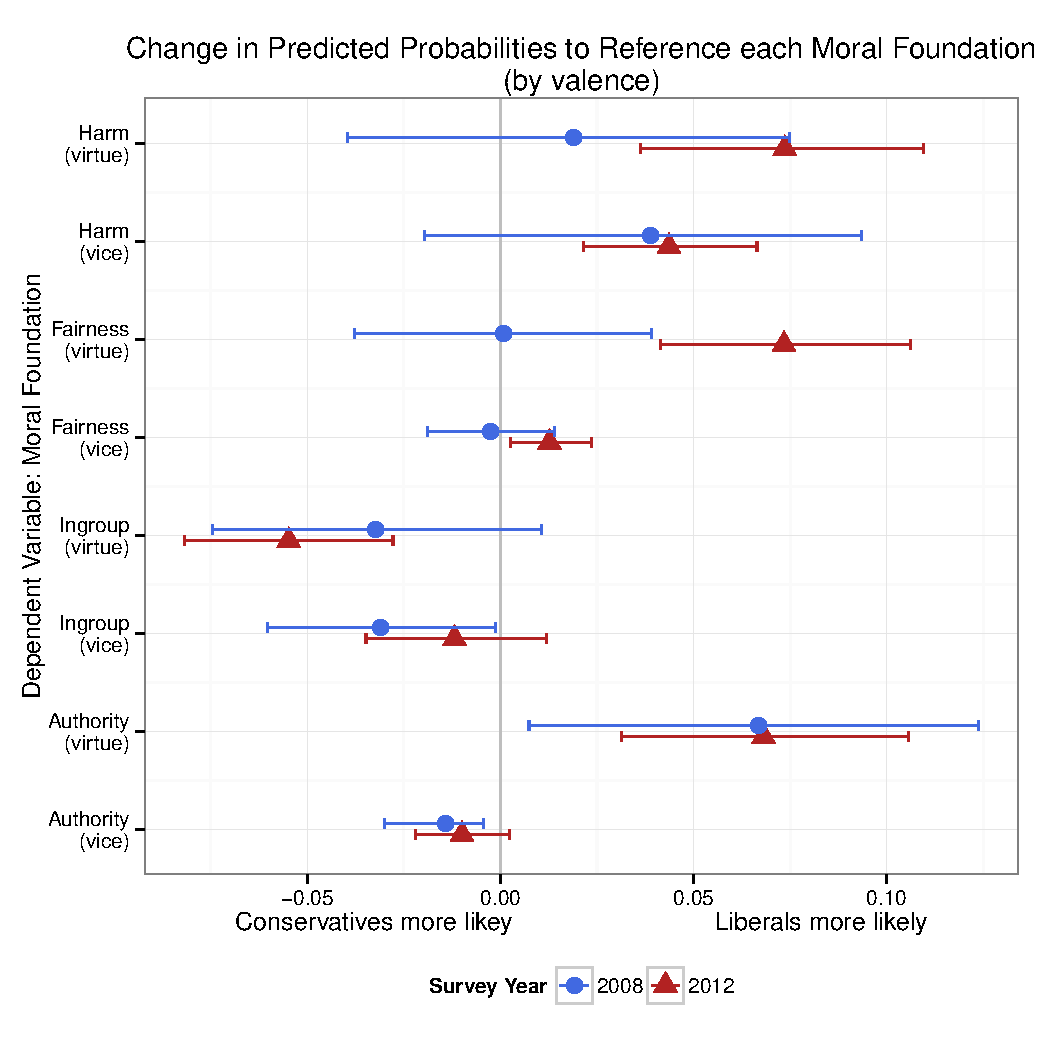
\includegraphics[scale=.4]{../calc/fig/appD4val.pdf}
\caption{Dis-aggregating moral foundations by valence. Full model results are reported in Tables \ref{tab:m2virtue} and \ref{tab:m2vice}.}\label{fig:appD4val}
  \end{subfigure}
  \begin{subfigure}[t]{0.49\textwidth}
    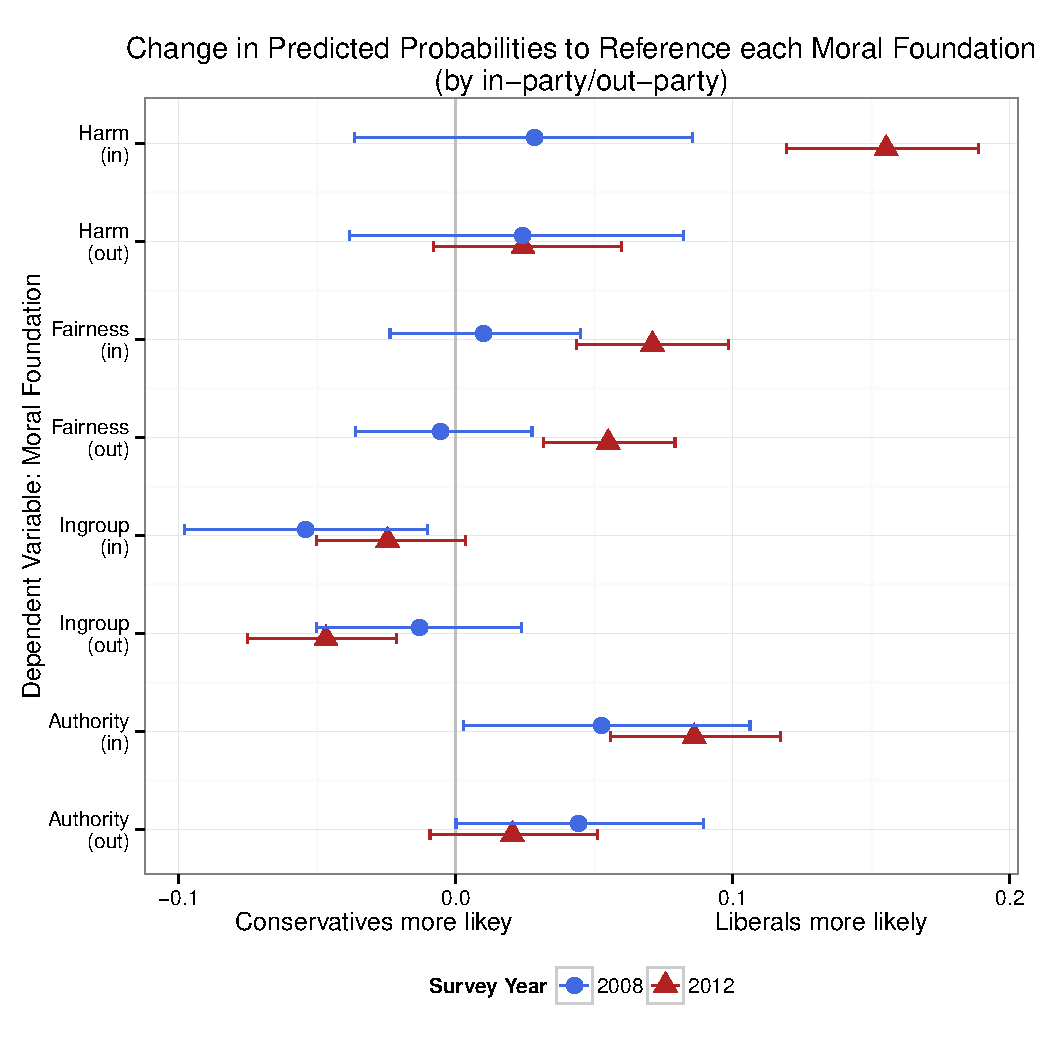
\includegraphics[scale=.4]{../calc/fig/appD5inout.pdf}
\caption{Dis-aggregating statements by in- and out-party. Full model results are reported in Tables \ref{tab:m2inparty} and \ref{tab:m2outparty}.}\label{fig:appD5inout}
  \end{subfigure}
  \begin{subfigure}[t]{0.49\textwidth}
    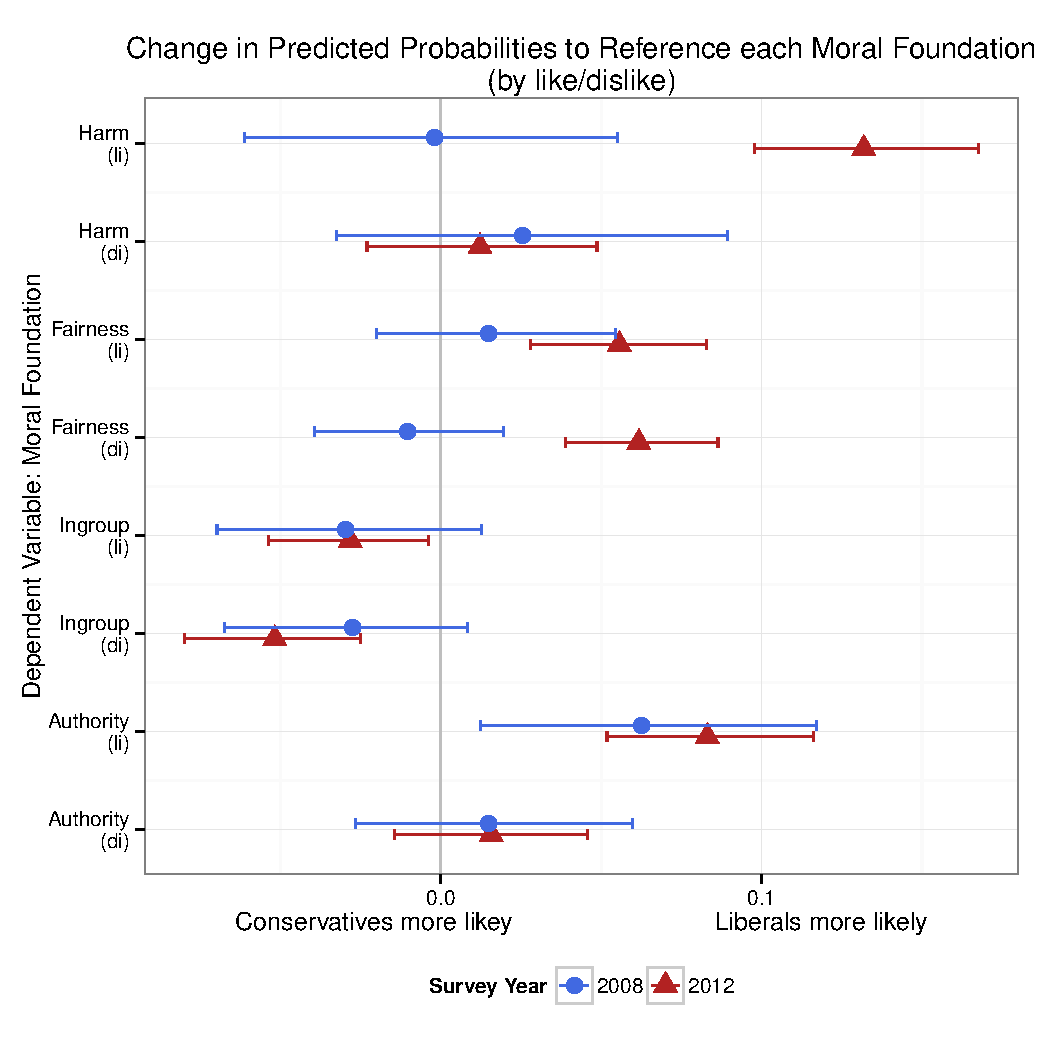
\includegraphics[scale=.4]{../calc/fig/appD6lidi.pdf}
\caption{Dis-aggregating statements by likes and dislikes. Full model results are reported in Tables \ref{tab:m2likes} and \ref{tab:m2dislikes}.}\label{fig:appD6lidi}
  \end{subfigure}
\end{figure}


\clearpage
\subsection{Determinants of moral reasoning including 2008 ANES data}

\begin{figure}[h]
  \centering
  \caption{Models predicting probabilities to reference any moral foundation including 2008 ANES data.}
  \begin{subfigure}[t]{0.49\textwidth}
    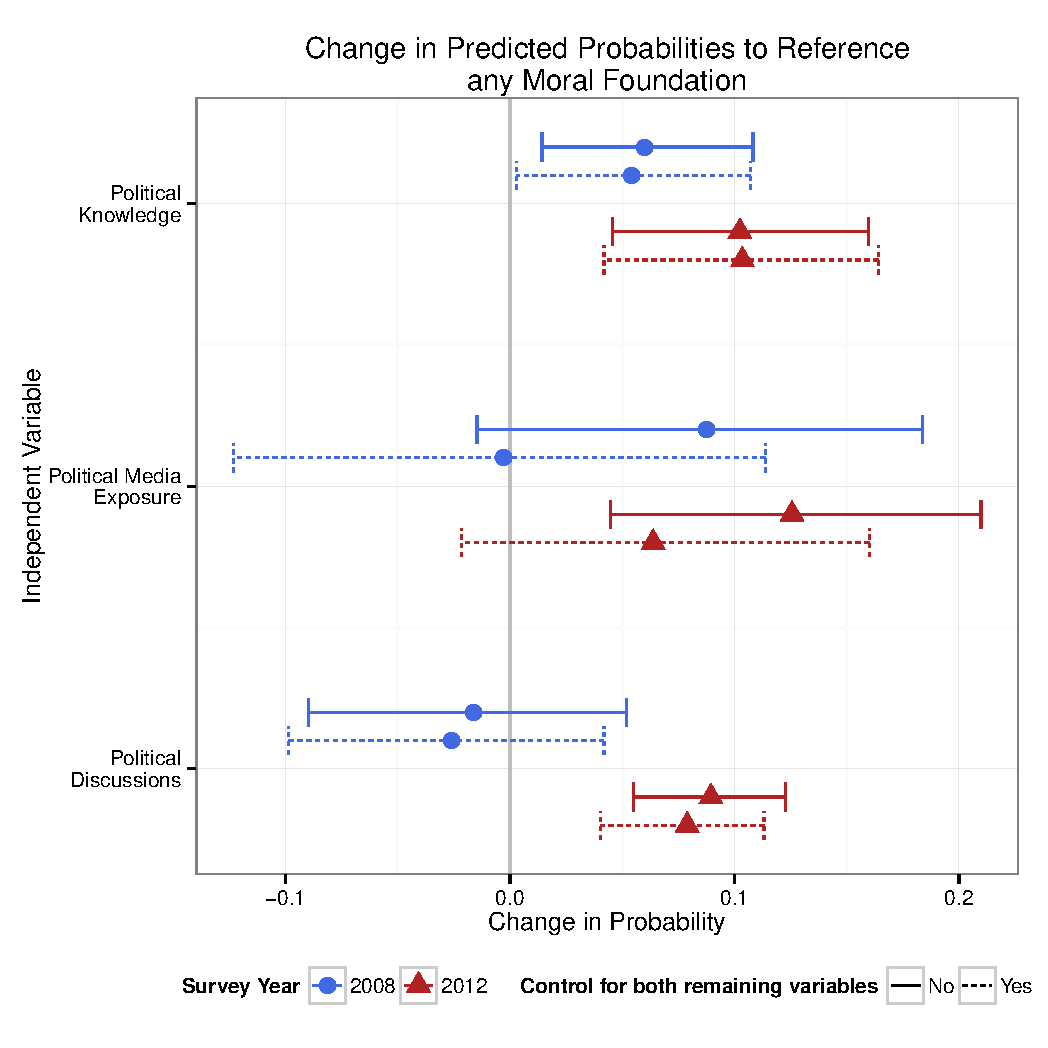
\includegraphics[scale=.4]{../calc/fig/appD7learn.pdf}
    \caption{Change in predicted probabilities to reference any moral foundation depending on political knowledge, media exposure, and frequency of political discussions. The plot shows the difference in predicted probabilities if each of the independent variables is increased from its minimum to its maximum value holding all other variables constant at their respective means (along with 95\% confidence intervals). Positive values indicate higher probabilities of referencing any moral foundation. Estimates are based on logit models and dotted lines indicate estimates while controlling for both remaining variables. Full model results are reported in Table \ref{tab:m3learn}.}\label{fig:appD7learn}
  \end{subfigure}
  \begin{subfigure}[t]{0.49\textwidth}
    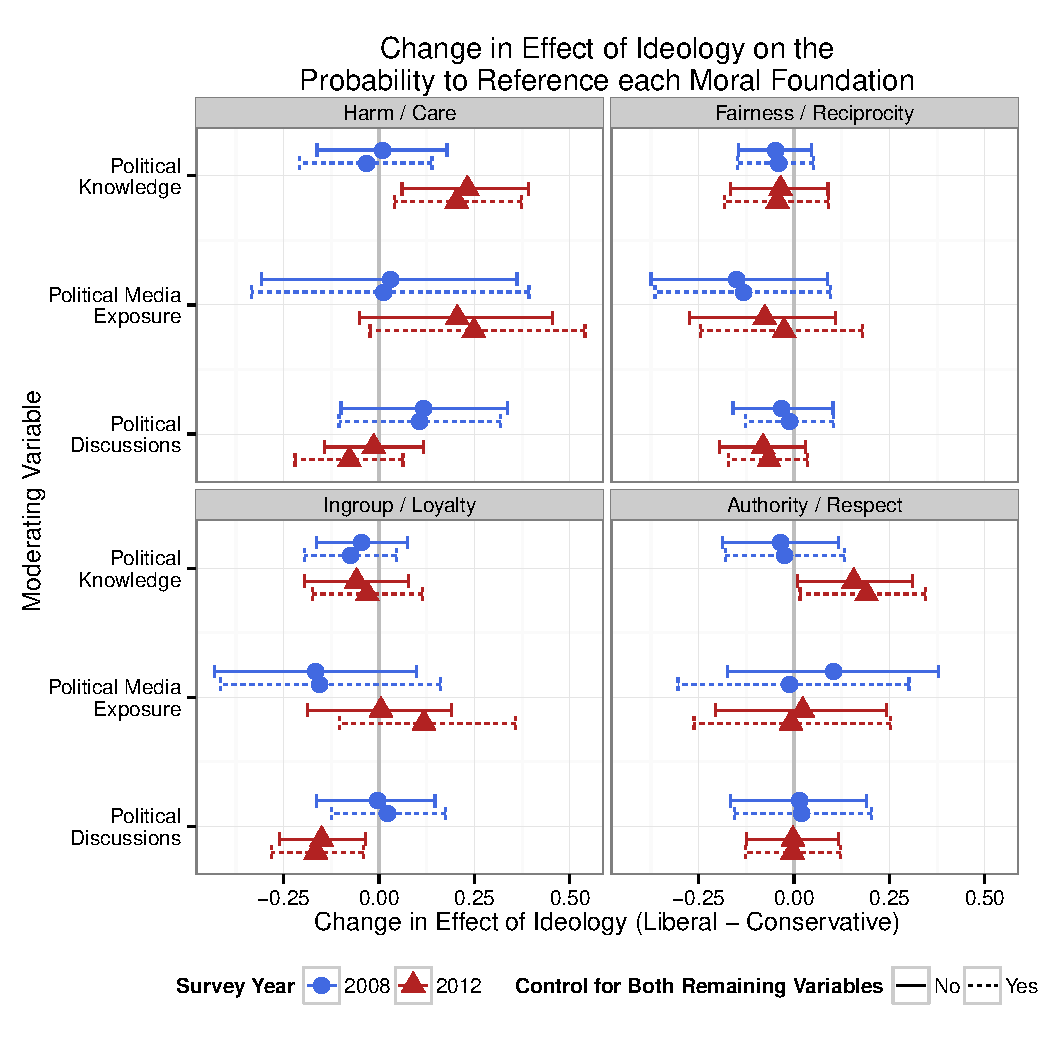
\includegraphics[scale=.4]{../calc/fig/appD8ideolearn.pdf}
    \caption{Change in effect of ideology on predicted probabilities to reference any moral foundation moderated by political knowledge, media exposure, and frequency of political discussions (difference-in-difference). The plot shows how the difference in predicted probabilities to reference each moral foundation between liberals and conservatives changes if each of the independent variables is increased from its minimum to its maximum value holding all other variables constant at their respective means (along with 95\% confidence intervals). Positive values indicate that liberals are more likely to mention a specific moral foundation if they score high on the moderating variable (knowledge, exposure, or discussions), and vice versa. Estimates are based on individual logit models for each foundation and dotted lines indicate estimates while controlling for both remaining variables. Full model results are reported in Tables \ref{tab:m4ideolearn2012a} to \ref{tab:m4ideolearn2008b}.}\label{fig:appD8ideolearn}
  \end{subfigure}
\end{figure}


\clearpage
\subsection{Consequences and political relevance of moral reasoning including 2008 ANES data}

\begin{figure}[h]
  \centering
  \caption{Models predicting turnout and protest behavior based on moral reasoning including 2008 ANES data.}
  \begin{subfigure}[t]{0.49\textwidth}
    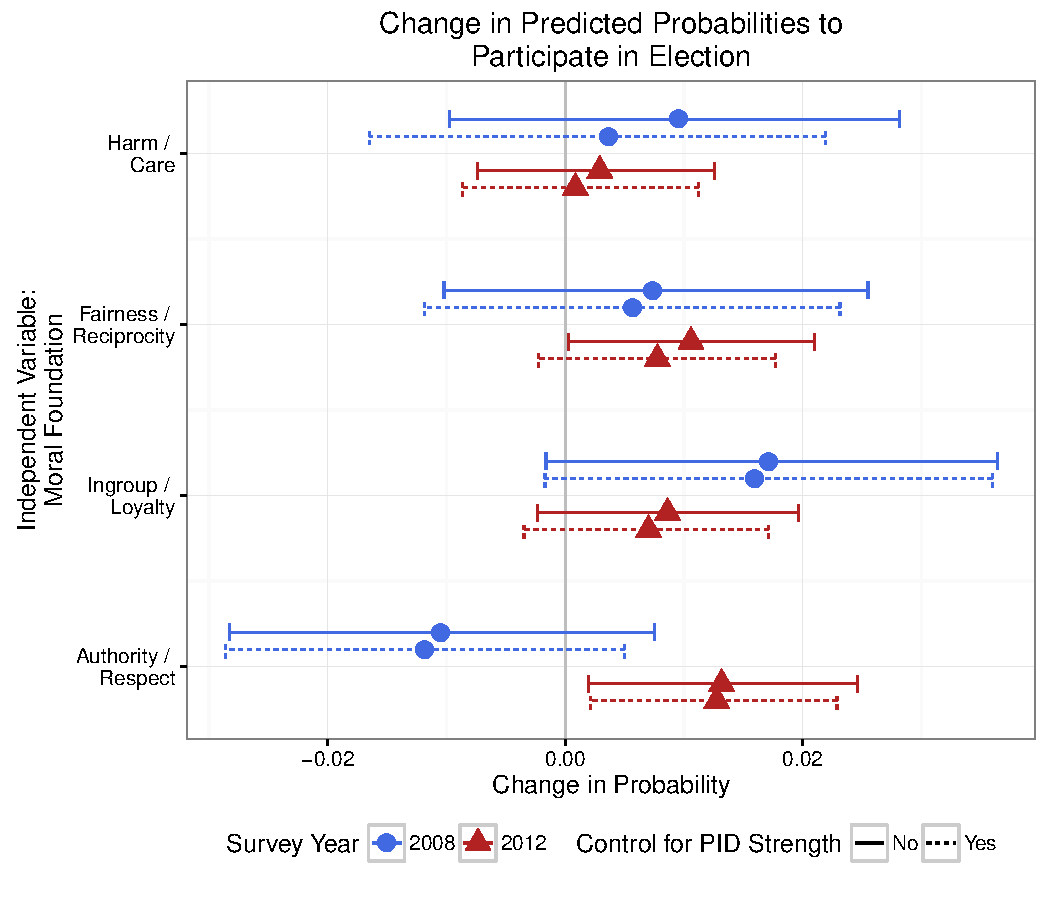
\includegraphics[scale=.4]{../calc/fig/appD9turnout.pdf}
    \caption{Difference in predicted probabilities to participate in election between respondents who mentioned each moral foundation or not, holding all other control variables constant at their respective means (along with 95\% confidence intervals). Positive values indicate that respondents who mentioned the respective foundation are more likely to participate in the election, and vice versa. Estimates are based on a single logit model including dichotomous indicators for each foundation and dotted lines indicate estimates while additionally controlling for the strength of party identification. Full model results are reported in Table \ref{tab:m5turnout}}\label{fig:appD9turnout}
  \end{subfigure}
  \begin{subfigure}[t]{0.49\textwidth}
    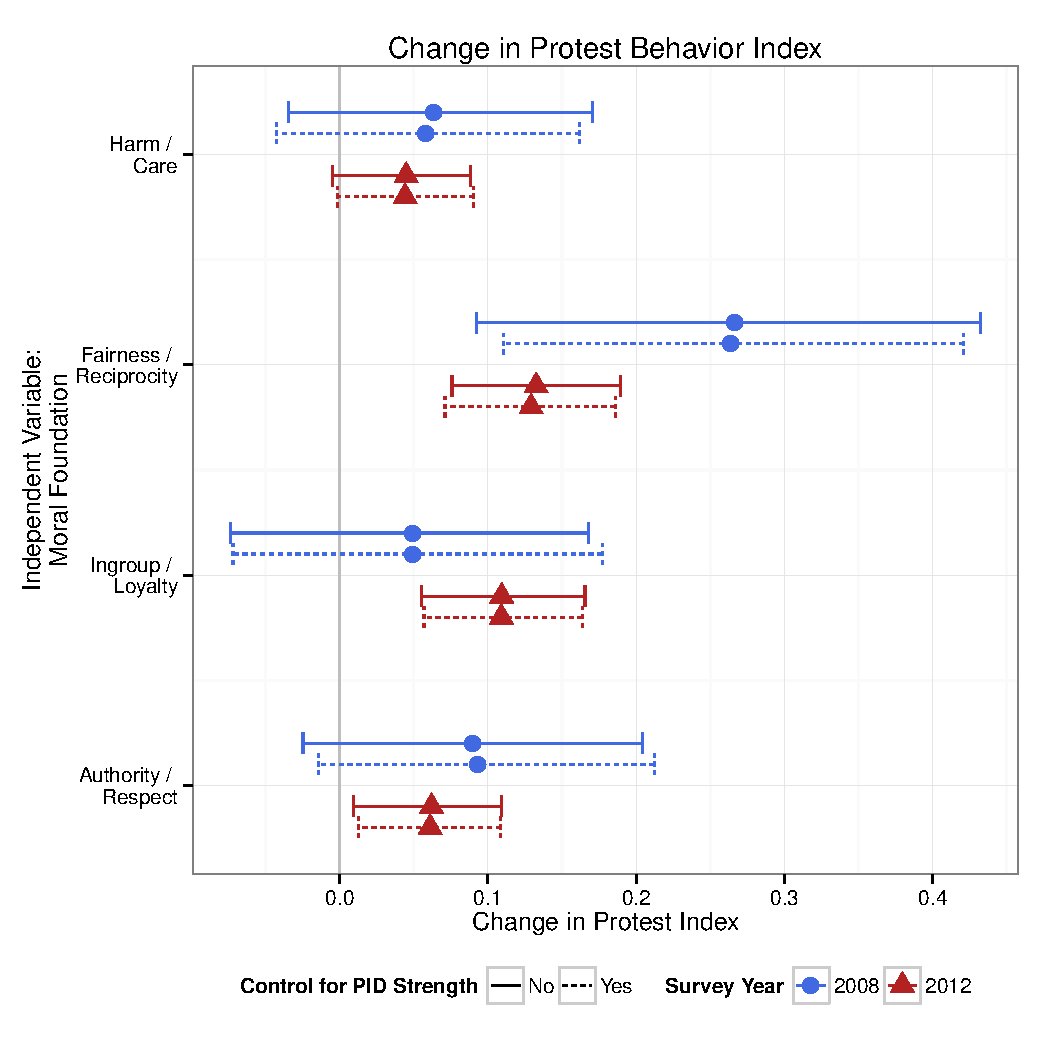
\includegraphics[scale=.4]{../calc/fig/appD10part.pdf}
    \caption{Difference in predicted protest behavior index between respondents who mentioned each moral foundation or not, holding all other control variables constant at their respective means (along with 95\% confidence intervals). Positive values indicate that respondents who mentioned the respective foundation scored higher on an additive protest behavior index ranging from 0 to 3, and vice versa. Estimates are based on a single OLS model (using robust standard errors) including dichotomous indicators for each foundation and dotted lines indicate estimates while additionally controlling for the strength of party identification. Full model results are reported in Table \ref{tab:m6part}.}\label{fig:appD10part}
  \end{subfigure}
\end{figure}
\begin{figure}[h]
  \centering
  \caption{Models predicting feeling thermometer differentials and vote choice based on moral reasoning including 2008 ANES data.}
  \begin{subfigure}[t]{0.49\textwidth}
    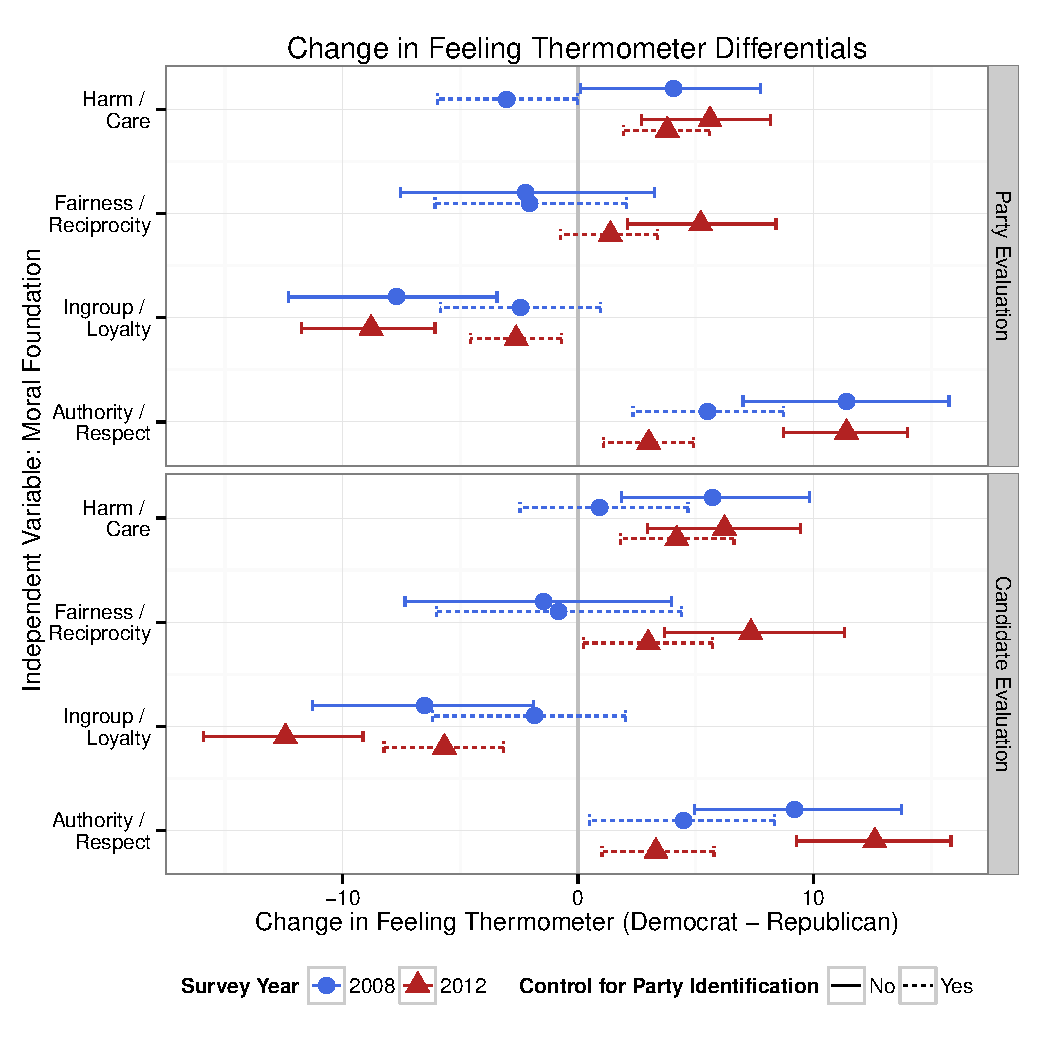
\includegraphics[scale=.4]{../calc/fig/appD11feel.pdf}
    \caption{Change in predicted feeling thermometer differential between respondents who mentioned each moral foundation or not, holding all other control variables constant at their respective means (along with 95\% confidence intervals). Positive values indicate that respondents who mentioned the respective foundation evaluated the Democratic candidate/party more favorably than the Republican candidate/party, and vice versa. Estimates are based on a single OLS model (using robust standard errors) including dichotomous indicators for each foundation and dotted lines indicate estimates while additionally controlling for party identification. Full model results are reported in Table \ref{tab:m7feel}.}\label{fig:appD11feel}
  \end{subfigure}
  \begin{subfigure}[t]{0.49\textwidth}
    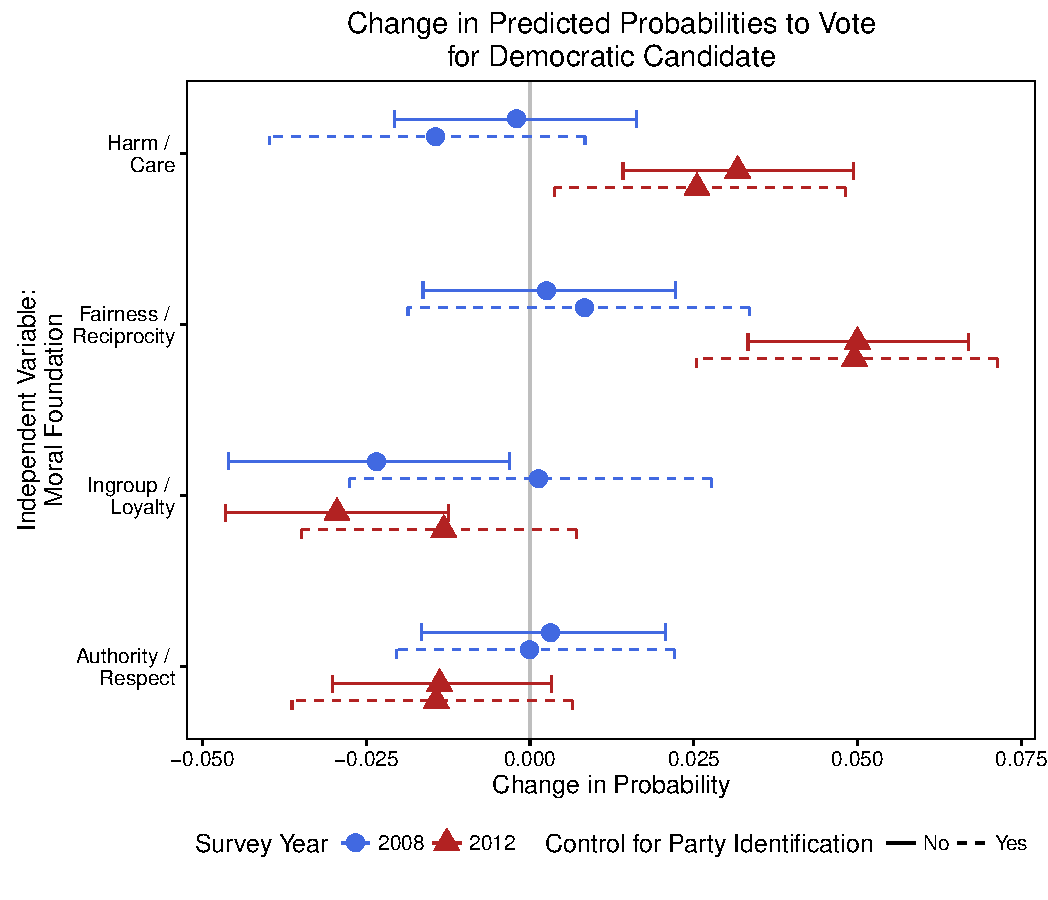
\includegraphics[scale=.4]{../calc/fig/appD12vote.pdf}
    \caption{Difference in predicted probabilities to vote for Democratic candidate between respondents who mentioned each moral foundation or not, holding all other control variables constant at their respective means (along with 95\% confidence intervals). Positive values indicate that respondents who mentioned the respective foundation are more likely to vote for the Democratic candidate, and vice versa. Estimates are based on a single logit model including dichotomous indicators for each foundation and dotted lines indicate estimates while additionally controlling for party identification. Full model results are reported in Table \ref{tab:m8vote}.}\label{fig:appD12vote}
  \end{subfigure}
\end{figure}


\clearpage
\section{Tables of Model Estimates}\label{app:tables}
\renewcommand\thefigure{\thesection.\arabic{figure}}
\renewcommand\thetable{\thesection.\arabic{table}}
\setcounter{figure}{0}
\setcounter{table}{0}


\subsection{Ideological differences in moral reasoning including 2008 ANES data}


% Table created by stargazer v.5.2 by Marek Hlavac, Harvard University. E-mail: hlavac at fas.harvard.edu
% Date and time: Wed, Jan 20, 2016 - 12:21:34 PM
% Requires LaTeX packages: dcolumn 
\begin{table}[ht] \centering 
  \caption{Logit Models Predicting References to four Moral Foundations using Ideology} 
  \label{tab:m2ideol} 
\tiny 
\begin{tabular}{@{\extracolsep{-15pt}}lD{.}{.}{-3} D{.}{.}{-3} D{.}{.}{-3} D{.}{.}{-3} D{.}{.}{-3} D{.}{.}{-3} D{.}{.}{-3} D{.}{.}{-3} } 
\\[-1.8ex]\hline 
\hline \\[-1.8ex] 
 & \multicolumn{8}{c}{\textit{Dependent variable:}} \\ 
\cline{2-9} 
\\[-1.8ex] & \multicolumn{2}{c}{Harm / Care} & \multicolumn{2}{c}{Fairness / Reciprocity} & \multicolumn{2}{c}{Ingroup / Loyalty} & \multicolumn{2}{c}{Authority / Respect} \\ 
 & \multicolumn{1}{c}{2012} & \multicolumn{1}{c}{2008} & \multicolumn{1}{c}{2012} & \multicolumn{1}{c}{2008} & \multicolumn{1}{c}{2012} & \multicolumn{1}{c}{2008} & \multicolumn{1}{c}{2012} & \multicolumn{1}{c}{2008} \\ 
\hline \\[-1.8ex] 
 Conservative & -0.340^{***} & -0.103 & -0.492^{***} & 0.019 & 0.298^{***} & 0.475^{***} & -0.272^{***} & -0.270^{*} \\ 
  & (0.083) & (0.148) & (0.092) & (0.191) & (0.090) & (0.171) & (0.085) & (0.152) \\ 
  Moderate & -0.338^{***} & -0.131 & -0.518^{***} & -0.273 & -0.026 & 0.367^{**} & -0.133 & -0.375^{**} \\ 
  & (0.084) & (0.150) & (0.094) & (0.209) & (0.095) & (0.178) & (0.085) & (0.159) \\ 
  Church Attendance & -0.016 & -0.039 & -0.0003 & -0.016 & 0.042^{**} & -0.012 & -0.030 & 0.052 \\ 
  & (0.019) & (0.035) & (0.022) & (0.046) & (0.021) & (0.039) & (0.020) & (0.036) \\ 
  Education (College Degree) & -0.017 & 0.139 & 0.322^{***} & 0.225 & 0.394^{***} & 0.554^{***} & 0.211^{***} & 0.321^{**} \\ 
  & (0.070) & (0.124) & (0.076) & (0.173) & (0.073) & (0.148) & (0.070) & (0.134) \\ 
  Age & -0.004^{*} & -0.015^{***} & 0.004^{*} & 0.011^{**} & -0.002 & -0.009^{**} & 0.007^{***} & -0.004 \\ 
  & (0.002) & (0.004) & (0.002) & (0.005) & (0.002) & (0.004) & (0.002) & (0.004) \\ 
  Sex (Female) & 0.200^{***} & 0.017 & 0.110 & 0.028 & -0.128^{*} & -0.432^{***} & -0.083 & -0.205^{*} \\ 
  & (0.066) & (0.118) & (0.074) & (0.157) & (0.072) & (0.134) & (0.067) & (0.124) \\ 
  Race (African American) & -0.017 & -0.066 & -0.103 & -0.042 & -0.189^{*} & -0.253 & 0.378^{***} & -0.081 \\ 
  & (0.091) & (0.150) & (0.105) & (0.207) & (0.103) & (0.180) & (0.091) & (0.160) \\ 
  Number of Words & 0.014^{***} & 0.017^{***} & 0.009^{***} & 0.008^{***} & 0.013^{***} & 0.015^{***} & 0.013^{***} & 0.011^{***} \\ 
  & (0.001) & (0.001) & (0.0005) & (0.001) & (0.001) & (0.001) & (0.001) & (0.001) \\ 
  Constant & -0.978^{***} & -0.614^{***} & -1.909^{***} & -3.026^{***} & -2.004^{***} & -2.071^{***} & -1.727^{***} & -1.366^{***} \\ 
  & (0.125) & (0.227) & (0.142) & (0.321) & (0.140) & (0.270) & (0.131) & (0.241) \\ 
 \hline \\[-1.8ex] 
Observations & \multicolumn{1}{c}{4,691} & \multicolumn{1}{c}{1,468} & \multicolumn{1}{c}{4,691} & \multicolumn{1}{c}{1,468} & \multicolumn{1}{c}{4,691} & \multicolumn{1}{c}{1,468} & \multicolumn{1}{c}{4,691} & \multicolumn{1}{c}{1,468} \\ 
Log Likelihood & \multicolumn{1}{c}{-2,765.763} & \multicolumn{1}{c}{-862.824} & \multicolumn{1}{c}{-2,310.347} & \multicolumn{1}{c}{-560.633} & \multicolumn{1}{c}{-2,440.218} & \multicolumn{1}{c}{-710.658} & \multicolumn{1}{c}{-2,702.758} & \multicolumn{1}{c}{-806.005} \\ 
Akaike Inf. Crit. & \multicolumn{1}{c}{5,549.527} & \multicolumn{1}{c}{1,743.648} & \multicolumn{1}{c}{4,638.693} & \multicolumn{1}{c}{1,139.266} & \multicolumn{1}{c}{4,898.436} & \multicolumn{1}{c}{1,439.317} & \multicolumn{1}{c}{5,423.517} & \multicolumn{1}{c}{1,630.010} \\ 
\hline 
\hline \\[-1.8ex] 
\textit{Note:}  & \multicolumn{8}{r}{$^{*}$p$<$0.1; $^{**}$p$<$0.05; $^{***}$p$<$0.01} \\ 
\end{tabular} 
\end{table} 


% Table created by stargazer v.5.2 by Marek Hlavac, Harvard University. E-mail: hlavac at fas.harvard.edu
% Date and time: Fri, Jan 22, 2016 - 04:19:28 PM
% Requires LaTeX packages: dcolumn 
\begin{table}[ht] \centering 
  \caption{Logit Models Predicting References to four Moral Foundations using Two-Dimensional Conceptualization of Ideology} 
  \label{tab:m2soceco} 
\tiny 
\begin{tabular}{@{\extracolsep{-15pt}}lD{.}{.}{-3} D{.}{.}{-3} D{.}{.}{-3} D{.}{.}{-3} D{.}{.}{-3} D{.}{.}{-3} D{.}{.}{-3} D{.}{.}{-3} } 
\\[-1.8ex]\hline 
\hline \\[-1.8ex] 
 & \multicolumn{8}{c}{\textit{Dependent variable:}} \\ 
\cline{2-9} 
\\[-1.8ex] & \multicolumn{2}{c}{Harm / Care} & \multicolumn{2}{c}{Fairness / Reciprocity} & \multicolumn{2}{c}{Ingroup / Loyalty} & \multicolumn{2}{c}{Authority / Respect} \\ 
 & \multicolumn{1}{c}{2012} & \multicolumn{1}{c}{2008} & \multicolumn{1}{c}{2012} & \multicolumn{1}{c}{2008} & \multicolumn{1}{c}{2012} & \multicolumn{1}{c}{2008} & \multicolumn{1}{c}{2012} & \multicolumn{1}{c}{2008} \\ 
\hline \\[-1.8ex] 
 Economic Liberalism & 0.430^{***} & 0.295 & 0.202 & -1.280^{***} & -0.730^{***} & -0.561^{**} & 0.388^{***} & 0.329 \\ 
  & (0.144) & (0.228) & (0.163) & (0.300) & (0.157) & (0.260) & (0.147) & (0.243) \\ 
  Social Liberalism & 0.174^{*} & -0.023 & 0.332^{***} & 0.430^{***} & -0.056 & -0.034 & 0.243^{**} & -0.026 \\ 
  & (0.104) & (0.112) & (0.120) & (0.157) & (0.114) & (0.133) & (0.106) & (0.121) \\ 
  Church Attendance & -0.010 & -0.029 & 0.010 & 0.034 & 0.043^{**} & 0.001 & -0.012 & 0.039 \\ 
  & (0.020) & (0.031) & (0.023) & (0.042) & (0.022) & (0.036) & (0.021) & (0.033) \\ 
  Education (College Degree) & 0.009 & 0.188^{*} & 0.387^{***} & 0.159 & 0.426^{***} & 0.474^{***} & 0.198^{***} & 0.363^{***} \\ 
  & (0.070) & (0.108) & (0.076) & (0.153) & (0.073) & (0.130) & (0.070) & (0.117) \\ 
  Age & -0.004^{*} & -0.012^{***} & 0.004^{*} & 0.013^{***} & -0.001 & -0.009^{**} & 0.006^{***} & -0.007^{**} \\ 
  & (0.002) & (0.003) & (0.002) & (0.004) & (0.002) & (0.004) & (0.002) & (0.003) \\ 
  Sex (Female) & 0.208^{***} & 0.028 & 0.099 & 0.094 & -0.166^{**} & -0.392^{***} & -0.117^{*} & -0.122 \\ 
  & (0.064) & (0.106) & (0.073) & (0.146) & (0.070) & (0.124) & (0.065) & (0.113) \\ 
  Race (African American) & -0.013 & -0.111 & -0.174^{*} & 0.205 & -0.132 & -0.099 & 0.367^{***} & -0.139 \\ 
  & (0.088) & (0.124) & (0.103) & (0.173) & (0.100) & (0.149) & (0.088) & (0.134) \\ 
  Number of Words & 0.014^{***} & 0.019^{***} & 0.009^{***} & 0.009^{***} & 0.013^{***} & 0.015^{***} & 0.013^{***} & 0.013^{***} \\ 
  & (0.001) & (0.001) & (0.0005) & (0.001) & (0.001) & (0.001) & (0.001) & (0.001) \\ 
  Constant & -1.595^{***} & -1.150^{***} & -2.634^{***} & -2.795^{***} & -1.602^{***} & -1.462^{***} & -2.163^{***} & -1.826^{***} \\ 
  & (0.149) & (0.252) & (0.172) & (0.350) & (0.160) & (0.291) & (0.154) & (0.273) \\ 
 \hline \\[-1.8ex] 
Observations & \multicolumn{1}{c}{4,970} & \multicolumn{1}{c}{1,908} & \multicolumn{1}{c}{4,970} & \multicolumn{1}{c}{1,908} & \multicolumn{1}{c}{4,970} & \multicolumn{1}{c}{1,908} & \multicolumn{1}{c}{4,970} & \multicolumn{1}{c}{1,908} \\ 
Log Likelihood & \multicolumn{1}{c}{-2,935.396} & \multicolumn{1}{c}{-1,109.287} & \multicolumn{1}{c}{-2,417.475} & \multicolumn{1}{c}{-678.629} & \multicolumn{1}{c}{-2,549.418} & \multicolumn{1}{c}{-870.335} & \multicolumn{1}{c}{-2,860.023} & \multicolumn{1}{c}{-1,004.710} \\ 
Akaike Inf. Crit. & \multicolumn{1}{c}{5,888.791} & \multicolumn{1}{c}{2,236.574} & \multicolumn{1}{c}{4,852.950} & \multicolumn{1}{c}{1,375.258} & \multicolumn{1}{c}{5,116.835} & \multicolumn{1}{c}{1,758.671} & \multicolumn{1}{c}{5,738.046} & \multicolumn{1}{c}{2,027.421} \\ 
\hline 
\hline \\[-1.8ex] 
\textit{Note:}  & \multicolumn{8}{r}{$^{*}$p$<$0.1; $^{**}$p$<$0.05; $^{***}$p$<$0.01} \\ 
\end{tabular} 
\end{table} 


% Table created by stargazer v.5.2 by Marek Hlavac, Harvard University. E-mail: hlavac at fas.harvard.edu
% Date and time: Wed, Jan 20, 2016 - 12:21:38 PM
% Requires LaTeX packages: dcolumn 
\begin{table}[ht] \centering 
  \caption{Logit Models Predicting References to four Moral Foundations using Ideology} 
  \label{tab:m2lead} 
\tiny 
\begin{tabular}{@{\extracolsep{-15pt}}lD{.}{.}{-3} D{.}{.}{-3} D{.}{.}{-3} D{.}{.}{-3} D{.}{.}{-3} D{.}{.}{-3} D{.}{.}{-3} D{.}{.}{-3} } 
\\[-1.8ex]\hline 
\hline \\[-1.8ex] 
 & \multicolumn{8}{c}{\textit{Dependent variable:}} \\ 
\cline{2-9} 
\\[-1.8ex] & \multicolumn{2}{c}{Harm / Care} & \multicolumn{2}{c}{Fairness / Reciprocity} & \multicolumn{2}{c}{Ingroup / Loyalty} & \multicolumn{2}{c}{Authority / Respect} \\ 
 & \multicolumn{1}{c}{2012} & \multicolumn{1}{c}{2008} & \multicolumn{1}{c}{2012} & \multicolumn{1}{c}{2008} & \multicolumn{1}{c}{2012} & \multicolumn{1}{c}{2008} & \multicolumn{1}{c}{2012} & \multicolumn{1}{c}{2008} \\ 
\hline \\[-1.8ex] 
 Conservative & -0.340^{***} & -0.103 & -0.492^{***} & 0.019 & 0.298^{***} & 0.475^{***} & -0.407^{***} & -0.270^{*} \\ 
  & (0.083) & (0.148) & (0.092) & (0.191) & (0.090) & (0.171) & (0.086) & (0.156) \\ 
  Moderate & -0.338^{***} & -0.131 & -0.518^{***} & -0.273 & -0.026 & 0.367^{**} & -0.178^{**} & -0.352^{**} \\ 
  & (0.084) & (0.150) & (0.094) & (0.209) & (0.095) & (0.178) & (0.085) & (0.163) \\ 
  Church Attendance & -0.016 & -0.039 & -0.0003 & -0.016 & 0.042^{**} & -0.012 & -0.034^{*} & 0.043 \\ 
  & (0.019) & (0.035) & (0.022) & (0.046) & (0.021) & (0.039) & (0.020) & (0.037) \\ 
  Education (College Degree) & -0.017 & 0.139 & 0.322^{***} & 0.225 & 0.394^{***} & 0.554^{***} & 0.138^{*} & 0.345^{**} \\ 
  & (0.070) & (0.124) & (0.076) & (0.173) & (0.073) & (0.148) & (0.071) & (0.138) \\ 
  Age & -0.004^{*} & -0.015^{***} & 0.004^{*} & 0.011^{**} & -0.002 & -0.009^{**} & 0.006^{***} & -0.006 \\ 
  & (0.002) & (0.004) & (0.002) & (0.005) & (0.002) & (0.004) & (0.002) & (0.004) \\ 
  Sex (Female) & 0.200^{***} & 0.017 & 0.110 & 0.028 & -0.128^{*} & -0.432^{***} & -0.051 & -0.192 \\ 
  & (0.066) & (0.118) & (0.074) & (0.157) & (0.072) & (0.134) & (0.068) & (0.127) \\ 
  Race (African American) & -0.017 & -0.066 & -0.103 & -0.042 & -0.189^{*} & -0.253 & 0.398^{***} & -0.076 \\ 
  & (0.091) & (0.150) & (0.105) & (0.207) & (0.103) & (0.180) & (0.091) & (0.164) \\ 
  Number of Words & 0.014^{***} & 0.017^{***} & 0.009^{***} & 0.008^{***} & 0.013^{***} & 0.015^{***} & 0.012^{***} & 0.010^{***} \\ 
  & (0.001) & (0.001) & (0.0005) & (0.001) & (0.001) & (0.001) & (0.001) & (0.001) \\ 
  Constant & -0.978^{***} & -0.614^{***} & -1.909^{***} & -3.026^{***} & -2.004^{***} & -2.071^{***} & -1.667^{***} & -1.394^{***} \\ 
  & (0.125) & (0.227) & (0.142) & (0.321) & (0.140) & (0.270) & (0.131) & (0.247) \\ 
 \hline \\[-1.8ex] 
Observations & \multicolumn{1}{c}{4,691} & \multicolumn{1}{c}{1,468} & \multicolumn{1}{c}{4,691} & \multicolumn{1}{c}{1,468} & \multicolumn{1}{c}{4,691} & \multicolumn{1}{c}{1,468} & \multicolumn{1}{c}{4,691} & \multicolumn{1}{c}{1,468} \\ 
Log Likelihood & \multicolumn{1}{c}{-2,765.763} & \multicolumn{1}{c}{-862.824} & \multicolumn{1}{c}{-2,310.347} & \multicolumn{1}{c}{-560.633} & \multicolumn{1}{c}{-2,440.218} & \multicolumn{1}{c}{-710.658} & \multicolumn{1}{c}{-2,658.051} & \multicolumn{1}{c}{-775.158} \\ 
Akaike Inf. Crit. & \multicolumn{1}{c}{5,549.527} & \multicolumn{1}{c}{1,743.648} & \multicolumn{1}{c}{4,638.693} & \multicolumn{1}{c}{1,139.266} & \multicolumn{1}{c}{4,898.436} & \multicolumn{1}{c}{1,439.317} & \multicolumn{1}{c}{5,334.102} & \multicolumn{1}{c}{1,568.316} \\ 
\hline 
\hline \\[-1.8ex] 
\textit{Note:}  & \multicolumn{8}{r}{$^{*}$p$<$0.1; $^{**}$p$<$0.05; $^{***}$p$<$0.01} \\ 
\end{tabular} 
\end{table} 


% Table created by stargazer v.5.2 by Marek Hlavac, Harvard University. E-mail: hlavac at fas.harvard.edu
% Date and time: Fri, Jan 22, 2016 - 11:53:58 PM
% Requires LaTeX packages: dcolumn 
\begin{table}[ht] \centering 
  \caption{Logit models predicting references to four moral foundations described as virtues using ideology} 
  \label{tab:m2virtue} 
\tiny 
\begin{tabular}{@{\extracolsep{-15pt}}lD{.}{.}{-3} D{.}{.}{-3} D{.}{.}{-3} D{.}{.}{-3} D{.}{.}{-3} D{.}{.}{-3} D{.}{.}{-3} D{.}{.}{-3} } 
\\[-1.8ex]\hline 
\hline \\[-1.8ex] 
 & \multicolumn{8}{c}{\textit{Dependent variable:}} \\ 
\cline{2-9} 
\\[-1.8ex] & \multicolumn{2}{c}{Harm / Care} & \multicolumn{2}{c}{Fairness / Reciprocity} & \multicolumn{2}{c}{Ingroup / Loyalty} & \multicolumn{2}{c}{Authority / Respect} \\ 
 & \multicolumn{1}{c}{2012} & \multicolumn{1}{c}{2008} & \multicolumn{1}{c}{2012} & \multicolumn{1}{c}{2008} & \multicolumn{1}{c}{2012} & \multicolumn{1}{c}{2008} & \multicolumn{1}{c}{2012} & \multicolumn{1}{c}{2008} \\ 
\hline \\[-1.8ex] 
 Conservative & -0.327^{***} & -0.105 & -0.440^{***} & -0.005 & 0.407^{***} & 0.288 & -0.308^{***} & -0.342^{**} \\ 
  & (0.084) & (0.160) & (0.093) & (0.198) & (0.104) & (0.192) & (0.085) & (0.153) \\ 
  Moderate & -0.383^{***} & -0.144 & -0.480^{***} & -0.280 & 0.133 & 0.158 & -0.129 & -0.442^{***} \\ 
  & (0.085) & (0.165) & (0.096) & (0.217) & (0.110) & (0.202) & (0.085) & (0.159) \\ 
  Church Attendance & -0.014 & -0.025 & 0.002 & -0.015 & 0.074^{***} & 0.052 & -0.026 & 0.064^{*} \\ 
  & (0.020) & (0.039) & (0.022) & (0.048) & (0.023) & (0.044) & (0.020) & (0.037) \\ 
  Education (College Degree) & 0.032 & 0.318^{**} & 0.315^{***} & 0.306^{*} & 0.138^{*} & 0.458^{***} & 0.235^{***} & 0.321^{**} \\ 
  & (0.070) & (0.140) & (0.077) & (0.182) & (0.083) & (0.171) & (0.070) & (0.134) \\ 
  Age & -0.004^{**} & -0.017^{***} & 0.003 & 0.010^{**} & 0.002 & 0.001 & 0.008^{***} & -0.004 \\ 
  & (0.002) & (0.004) & (0.002) & (0.005) & (0.002) & (0.005) & (0.002) & (0.004) \\ 
  Sex (Female) & 0.274^{***} & 0.074 & 0.133^{*} & 0.154 & -0.007 & -0.085 & -0.069 & -0.182 \\ 
  & (0.067) & (0.129) & (0.076) & (0.164) & (0.081) & (0.152) & (0.067) & (0.124) \\ 
  Race (African American) & -0.028 & -0.044 & -0.139 & -0.102 & 0.012 & 0.235 & 0.417^{***} & -0.071 \\ 
  & (0.092) & (0.166) & (0.108) & (0.219) & (0.114) & (0.191) & (0.091) & (0.160) \\ 
  Number of Words & 0.011^{***} & 0.013^{***} & 0.008^{***} & 0.008^{***} & 0.011^{***} & 0.011^{***} & 0.012^{***} & 0.010^{***} \\ 
  & (0.001) & (0.001) & (0.0005) & (0.001) & (0.001) & (0.001) & (0.001) & (0.001) \\ 
  Constant & -1.108^{***} & -1.193^{***} & -1.935^{***} & -3.164^{***} & -2.839^{***} & -3.062^{***} & -1.811^{***} & -1.362^{***} \\ 
  & (0.126) & (0.249) & (0.144) & (0.335) & (0.163) & (0.315) & (0.132) & (0.241) \\ 
 \hline \\[-1.8ex] 
Observations & \multicolumn{1}{c}{4,691} & \multicolumn{1}{c}{1,468} & \multicolumn{1}{c}{4,691} & \multicolumn{1}{c}{1,468} & \multicolumn{1}{c}{4,691} & \multicolumn{1}{c}{1,468} & \multicolumn{1}{c}{4,691} & \multicolumn{1}{c}{1,468} \\ 
Log Likelihood & \multicolumn{1}{c}{-2,718.587} & \multicolumn{1}{c}{-754.236} & \multicolumn{1}{c}{-2,251.633} & \multicolumn{1}{c}{-528.080} & \multicolumn{1}{c}{-2,015.282} & \multicolumn{1}{c}{-586.828} & \multicolumn{1}{c}{-2,684.276} & \multicolumn{1}{c}{-802.048} \\ 
Akaike Inf. Crit. & \multicolumn{1}{c}{5,455.174} & \multicolumn{1}{c}{1,526.472} & \multicolumn{1}{c}{4,521.265} & \multicolumn{1}{c}{1,074.159} & \multicolumn{1}{c}{4,048.565} & \multicolumn{1}{c}{1,191.656} & \multicolumn{1}{c}{5,386.553} & \multicolumn{1}{c}{1,622.097} \\ 
\hline 
\hline \\[-1.8ex] 
\textit{Note:}  & \multicolumn{8}{r}{$^{*}$p$<$0.1; $^{**}$p$<$0.05; $^{***}$p$<$0.01} \\ 
\end{tabular} 
\end{table} 


% Table created by stargazer v.5.2 by Marek Hlavac, Harvard University. E-mail: hlavac at fas.harvard.edu
% Date and time: Fri, Jan 22, 2016 - 04:19:34 PM
% Requires LaTeX packages: dcolumn 
\begin{table}[ht] \centering 
  \caption{Logit Models Predicting References to four Moral Foundations using Ideology (vices)} 
  \label{tab:m2vice} 
\tiny 
\begin{tabular}{@{\extracolsep{-15pt}}lD{.}{.}{-3} D{.}{.}{-3} D{.}{.}{-3} D{.}{.}{-3} D{.}{.}{-3} D{.}{.}{-3} D{.}{.}{-3} D{.}{.}{-3} } 
\\[-1.8ex]\hline 
\hline \\[-1.8ex] 
 & \multicolumn{8}{c}{\textit{Dependent variable:}} \\ 
\cline{2-9} 
\\[-1.8ex] & \multicolumn{2}{c}{Harm / Care} & \multicolumn{2}{c}{Fairness / Reciprocity} & \multicolumn{2}{c}{Ingroup / Loyalty} & \multicolumn{2}{c}{Authority / Respect} \\ 
 & \multicolumn{1}{c}{2012} & \multicolumn{1}{c}{2008} & \multicolumn{1}{c}{2012} & \multicolumn{1}{c}{2008} & \multicolumn{1}{c}{2012} & \multicolumn{1}{c}{2008} & \multicolumn{1}{c}{2012} & \multicolumn{1}{c}{2008} \\ 
\hline \\[-1.8ex] 
 Conservative & -0.454^{***} & -0.217 & -0.563^{**} & 0.161 & 0.110 & 0.412^{**} & 0.294 & 1.826^{***} \\ 
  & (0.118) & (0.159) & (0.222) & (0.459) & (0.107) & (0.207) & (0.186) & (0.655) \\ 
  Moderate & -0.192^{*} & -0.131 & -0.529^{**} & -0.641 & -0.232^{**} & 0.242 & -0.151 & 0.813 \\ 
  & (0.117) & (0.161) & (0.237) & (0.579) & (0.118) & (0.221) & (0.211) & (0.752) \\ 
  Church Attendance & 0.0004 & -0.026 & 0.011 & -0.023 & -0.033 & -0.110^{**} & -0.084^{*} & -0.106 \\ 
  & (0.028) & (0.038) & (0.054) & (0.113) & (0.026) & (0.050) & (0.045) & (0.117) \\ 
  Education (College Degree) & -0.089 & 0.030 & 0.277 & -0.276 & 0.661^{***} & 0.896^{***} & -0.070 & 1.136^{**} \\ 
  & (0.098) & (0.137) & (0.188) & (0.414) & (0.088) & (0.200) & (0.158) & (0.558) \\ 
  Age & 0.001 & -0.013^{***} & 0.010^{*} & 0.011 & -0.004 & -0.012^{**} & -0.0001 & -0.010 \\ 
  & (0.003) & (0.004) & (0.006) & (0.012) & (0.003) & (0.005) & (0.005) & (0.013) \\ 
  Sex (Female) & -0.103 & 0.141 & -0.200 & -0.742^{*} & -0.169^{*} & -0.885^{***} & -0.149 & -0.752^{*} \\ 
  & (0.094) & (0.128) & (0.186) & (0.409) & (0.088) & (0.170) & (0.153) & (0.427) \\ 
  Race (African American) & 0.129 & -0.065 & 0.030 & 0.007 & -0.482^{***} & -0.878^{***} & 0.019 & -1.405 \\ 
  & (0.126) & (0.163) & (0.258) & (0.524) & (0.141) & (0.270) & (0.220) & (1.035) \\ 
  Number of Words & 0.010^{***} & 0.011^{***} & 0.006^{***} & 0.006^{***} & 0.008^{***} & 0.008^{***} & 0.008^{***} & 0.006^{***} \\ 
  & (0.001) & (0.001) & (0.001) & (0.001) & (0.0005) & (0.001) & (0.001) & (0.001) \\ 
  Constant & -2.575^{***} & -1.111^{***} & -4.349^{***} & -4.439^{***} & -2.271^{***} & -2.097^{***} & -3.768^{***} & -5.449^{***} \\ 
  & (0.177) & (0.245) & (0.365) & (0.763) & (0.168) & (0.329) & (0.295) & (0.974) \\ 
 \hline \\[-1.8ex] 
Observations & \multicolumn{1}{c}{4,691} & \multicolumn{1}{c}{1,468} & \multicolumn{1}{c}{4,691} & \multicolumn{1}{c}{1,468} & \multicolumn{1}{c}{4,691} & \multicolumn{1}{c}{1,468} & \multicolumn{1}{c}{4,691} & \multicolumn{1}{c}{1,468} \\ 
Log Likelihood & \multicolumn{1}{c}{-1,604.663} & \multicolumn{1}{c}{-768.760} & \multicolumn{1}{c}{-546.345} & \multicolumn{1}{c}{-129.201} & \multicolumn{1}{c}{-1,788.764} & \multicolumn{1}{c}{-506.576} & \multicolumn{1}{c}{-742.173} & \multicolumn{1}{c}{-115.922} \\ 
Akaike Inf. Crit. & \multicolumn{1}{c}{3,227.327} & \multicolumn{1}{c}{1,555.520} & \multicolumn{1}{c}{1,110.691} & \multicolumn{1}{c}{276.403} & \multicolumn{1}{c}{3,595.528} & \multicolumn{1}{c}{1,031.153} & \multicolumn{1}{c}{1,502.346} & \multicolumn{1}{c}{249.843} \\ 
\hline 
\hline \\[-1.8ex] 
\textit{Note:}  & \multicolumn{8}{r}{$^{*}$p$<$0.1; $^{**}$p$<$0.05; $^{***}$p$<$0.01} \\ 
\end{tabular} 
\end{table} 


% Table created by stargazer v.5.2 by Marek Hlavac, Harvard University. E-mail: hlavac at fas.harvard.edu
% Date and time: Sat, Jan 23, 2016 - 02:23:09 PM
% Requires LaTeX packages: dcolumn 
\begin{table}[ht] \centering 
  \caption{Logit models predicting references to four moral foundations describing in-party using ideology} 
  \label{tab:m2inparty} 
\tiny 
\begin{tabular}{@{\extracolsep{-15pt}}lD{.}{.}{-3} D{.}{.}{-3} D{.}{.}{-3} D{.}{.}{-3} D{.}{.}{-3} D{.}{.}{-3} D{.}{.}{-3} D{.}{.}{-3} } 
\\[-1.8ex]\hline 
\hline \\[-1.8ex] 
 & \multicolumn{8}{c}{\textit{Dependent variable:}} \\ 
\cline{2-9} 
\\[-1.8ex] & \multicolumn{2}{c}{Harm / Care} & \multicolumn{2}{c}{Fairness / Reciprocity} & \multicolumn{2}{c}{Ingroup / Loyalty} & \multicolumn{2}{c}{Authority / Respect} \\ 
 & \multicolumn{1}{c}{2012} & \multicolumn{1}{c}{2008} & \multicolumn{1}{c}{2012} & \multicolumn{1}{c}{2008} & \multicolumn{1}{c}{2012} & \multicolumn{1}{c}{2008} & \multicolumn{1}{c}{2012} & \multicolumn{1}{c}{2008} \\ 
\hline \\[-1.8ex] 
 Conservative & -0.785^{***} & -0.141 & -0.529^{***} & -0.129 & 0.171^{*} & 0.464^{**} & -0.478^{***} & -0.319^{**} \\ 
  & (0.089) & (0.156) & (0.102) & (0.222) & (0.101) & (0.186) & (0.091) & (0.163) \\ 
  Moderate & -0.486^{***} & -0.207 & -0.432^{***} & -0.400 & -0.042 & 0.330^{*} & -0.246^{***} & -0.488^{***} \\ 
  & (0.088) & (0.162) & (0.105) & (0.248) & (0.107) & (0.195) & (0.091) & (0.174) \\ 
  Church Attendance & -0.042^{**} & -0.022 & -0.016 & -0.002 & 0.048^{**} & -0.011 & 0.005 & 0.057 \\ 
  & (0.021) & (0.038) & (0.024) & (0.054) & (0.023) & (0.043) & (0.021) & (0.040) \\ 
  Education (College Degree) & -0.039 & 0.129 & 0.285^{***} & 0.273 & 0.303^{***} & 0.625^{***} & 0.161^{**} & 0.119 \\ 
  & (0.075) & (0.136) & (0.085) & (0.208) & (0.082) & (0.166) & (0.075) & (0.145) \\ 
  Age & -0.005^{**} & -0.021^{***} & 0.005^{**} & 0.012^{**} & -0.002 & -0.011^{**} & 0.008^{***} & -0.006 \\ 
  & (0.002) & (0.004) & (0.003) & (0.006) & (0.002) & (0.005) & (0.002) & (0.004) \\ 
  Sex (Female) & 0.155^{**} & 0.042 & 0.105 & 0.168 & -0.075 & -0.416^{***} & -0.082 & -0.087 \\ 
  & (0.071) & (0.127) & (0.083) & (0.188) & (0.081) & (0.146) & (0.073) & (0.134) \\ 
  Race (African American) & 0.026 & -0.379^{**} & -0.088 & 0.239 & -0.058 & -0.012 & 0.184^{*} & -0.031 \\ 
  & (0.097) & (0.167) & (0.117) & (0.234) & (0.114) & (0.191) & (0.097) & (0.172) \\ 
  Number of Words & 0.009^{***} & 0.012^{***} & 0.006^{***} & 0.007^{***} & 0.010^{***} & 0.009^{***} & 0.008^{***} & 0.006^{***} \\ 
  & (0.001) & (0.001) & (0.0005) & (0.001) & (0.001) & (0.001) & (0.0005) & (0.001) \\ 
  Constant & -0.956^{***} & -0.591^{**} & -2.193^{***} & -3.531^{***} & -2.342^{***} & -2.113^{***} & -1.915^{***} & -1.317^{***} \\ 
  & (0.133) & (0.242) & (0.160) & (0.386) & (0.158) & (0.293) & (0.141) & (0.258) \\ 
 \hline \\[-1.8ex] 
Observations & \multicolumn{1}{c}{4,470} & \multicolumn{1}{c}{1,429} & \multicolumn{1}{c}{4,470} & \multicolumn{1}{c}{1,429} & \multicolumn{1}{c}{4,470} & \multicolumn{1}{c}{1,429} & \multicolumn{1}{c}{4,470} & \multicolumn{1}{c}{1,429} \\ 
Log Likelihood & \multicolumn{1}{c}{-2,419.933} & \multicolumn{1}{c}{-774.173} & \multicolumn{1}{c}{-1,931.938} & \multicolumn{1}{c}{-427.785} & \multicolumn{1}{c}{-2,010.597} & \multicolumn{1}{c}{-619.785} & \multicolumn{1}{c}{-2,375.317} & \multicolumn{1}{c}{-708.737} \\ 
Akaike Inf. Crit. & \multicolumn{1}{c}{4,857.867} & \multicolumn{1}{c}{1,566.346} & \multicolumn{1}{c}{3,881.876} & \multicolumn{1}{c}{873.570} & \multicolumn{1}{c}{4,039.195} & \multicolumn{1}{c}{1,257.570} & \multicolumn{1}{c}{4,768.633} & \multicolumn{1}{c}{1,435.473} \\ 
\hline 
\hline \\[-1.8ex] 
\textit{Note:}  & \multicolumn{8}{r}{$^{*}$p$<$0.1; $^{**}$p$<$0.05; $^{***}$p$<$0.01} \\ 
\end{tabular} 
\end{table} 


% Table created by stargazer v.5.2 by Marek Hlavac, Harvard University. E-mail: hlavac at fas.harvard.edu
% Date and time: Wed, Jan 20, 2016 - 05:28:29 PM
% Requires LaTeX packages: dcolumn 
\begin{table}[ht] \centering 
  \caption{Logit Models Predicting References to four Moral Foundations using Ideology (out-party)} 
  \label{tab:m2outparty} 
\tiny 
\begin{tabular}{@{\extracolsep{-15pt}}lD{.}{.}{-3} D{.}{.}{-3} D{.}{.}{-3} D{.}{.}{-3} D{.}{.}{-3} D{.}{.}{-3} D{.}{.}{-3} D{.}{.}{-3} } 
\\[-1.8ex]\hline 
\hline \\[-1.8ex] 
 & \multicolumn{8}{c}{\textit{Dependent variable:}} \\ 
\cline{2-9} 
\\[-1.8ex] & \multicolumn{2}{c}{Harm / Care} & \multicolumn{2}{c}{Fairness / Reciprocity} & \multicolumn{2}{c}{Ingroup / Loyalty} & \multicolumn{2}{c}{Authority / Respect} \\ 
 & \multicolumn{1}{c}{2012} & \multicolumn{1}{c}{2008} & \multicolumn{1}{c}{2012} & \multicolumn{1}{c}{2008} & \multicolumn{1}{c}{2012} & \multicolumn{1}{c}{2008} & \multicolumn{1}{c}{2012} & \multicolumn{1}{c}{2008} \\ 
\hline \\[-1.8ex] 
 Conservative & -0.124 & -0.133 & -0.531^{***} & 0.092 & 0.335^{***} & 0.138 & -0.122 & -0.390^{**} \\ 
  & (0.089) & (0.163) & (0.114) & (0.252) & (0.101) & (0.204) & (0.094) & (0.191) \\ 
  Moderate & -0.195^{**} & 0.039 & -0.438^{***} & -0.349 & 0.044 & 0.172 & -0.021 & -0.297 \\ 
  & (0.092) & (0.164) & (0.118) & (0.291) & (0.109) & (0.213) & (0.096) & (0.200) \\ 
  Church Attendance & 0.021 & -0.049 & -0.001 & -0.018 & 0.015 & -0.003 & -0.036 & 0.093^{**} \\ 
  & (0.021) & (0.039) & (0.028) & (0.062) & (0.023) & (0.048) & (0.022) & (0.045) \\ 
  Education (College Degree) & -0.022 & 0.213 & 0.345^{***} & 0.282 & 0.379^{***} & 0.523^{***} & 0.223^{***} & 0.634^{***} \\ 
  & (0.074) & (0.141) & (0.094) & (0.240) & (0.081) & (0.188) & (0.077) & (0.182) \\ 
  Age & -0.006^{***} & -0.019^{***} & -0.007^{**} & -0.0003 & -0.003 & -0.014^{***} & 0.006^{***} & -0.003 \\ 
  & (0.002) & (0.004) & (0.003) & (0.006) & (0.002) & (0.005) & (0.002) & (0.005) \\ 
  Sex (Female) & 0.155^{**} & 0.052 & 0.129 & 0.071 & -0.129 & -0.429^{***} & -0.092 & -0.277^{*} \\ 
  & (0.071) & (0.130) & (0.094) & (0.211) & (0.081) & (0.163) & (0.075) & (0.155) \\ 
  Race (African American) & -0.193^{*} & 0.149 & -0.486^{***} & -0.329 & -0.521^{***} & -0.619^{**} & 0.309^{***} & -0.131 \\ 
  & (0.101) & (0.165) & (0.146) & (0.308) & (0.128) & (0.242) & (0.101) & (0.207) \\ 
  Number of Words & 0.008^{***} & 0.011^{***} & 0.007^{***} & 0.005^{***} & 0.008^{***} & 0.011^{***} & 0.009^{***} & 0.009^{***} \\ 
  & (0.0005) & (0.001) & (0.0005) & (0.001) & (0.0005) & (0.001) & (0.001) & (0.001) \\ 
  Constant & -1.313^{***} & -0.898^{***} & -1.946^{***} & -3.026^{***} & -2.176^{***} & -2.072^{***} & -2.191^{***} & -2.380^{***} \\ 
  & (0.134) & (0.251) & (0.172) & (0.420) & (0.157) & (0.322) & (0.147) & (0.313) \\ 
 \hline \\[-1.8ex] 
Observations & \multicolumn{1}{c}{4,469} & \multicolumn{1}{c}{1,371} & \multicolumn{1}{c}{4,469} & \multicolumn{1}{c}{1,371} & \multicolumn{1}{c}{4,469} & \multicolumn{1}{c}{1,371} & \multicolumn{1}{c}{4,469} & \multicolumn{1}{c}{1,371} \\ 
Log Likelihood & \multicolumn{1}{c}{-2,460.166} & \multicolumn{1}{c}{-737.700} & \multicolumn{1}{c}{-1,606.607} & \multicolumn{1}{c}{-353.620} & \multicolumn{1}{c}{-2,025.254} & \multicolumn{1}{c}{-521.419} & \multicolumn{1}{c}{-2,272.003} & \multicolumn{1}{c}{-561.110} \\ 
Akaike Inf. Crit. & \multicolumn{1}{c}{4,938.333} & \multicolumn{1}{c}{1,493.400} & \multicolumn{1}{c}{3,231.214} & \multicolumn{1}{c}{725.240} & \multicolumn{1}{c}{4,068.508} & \multicolumn{1}{c}{1,060.838} & \multicolumn{1}{c}{4,562.006} & \multicolumn{1}{c}{1,140.219} \\ 
\hline 
\hline \\[-1.8ex] 
\textit{Note:}  & \multicolumn{8}{r}{$^{*}$p$<$0.1; $^{**}$p$<$0.05; $^{***}$p$<$0.01} \\ 
\end{tabular} 
\end{table} 


% Table created by stargazer v.5.2 by Marek Hlavac, Harvard University. E-mail: hlavac at fas.harvard.edu
% Date and time: Wed, Jan 20, 2016 - 12:21:52 PM
% Requires LaTeX packages: dcolumn 
\begin{table}[ht] \centering 
  \caption{Logit Models Predicting References to four Moral Foundations using Ideology (dislikes)} 
  \label{tab:m2likes} 
\tiny 
\begin{tabular}{@{\extracolsep{-15pt}}lD{.}{.}{-3} D{.}{.}{-3} D{.}{.}{-3} D{.}{.}{-3} D{.}{.}{-3} D{.}{.}{-3} D{.}{.}{-3} D{.}{.}{-3} } 
\\[-1.8ex]\hline 
\hline \\[-1.8ex] 
 & \multicolumn{8}{c}{\textit{Dependent variable:}} \\ 
\cline{2-9} 
\\[-1.8ex] & \multicolumn{2}{c}{Harm / Care} & \multicolumn{2}{c}{Fairness / Reciprocity} & \multicolumn{2}{c}{Ingroup / Loyalty} & \multicolumn{2}{c}{Authority / Respect} \\ 
 & \multicolumn{1}{c}{2012} & \multicolumn{1}{c}{2008} & \multicolumn{1}{c}{2012} & \multicolumn{1}{c}{2008} & \multicolumn{1}{c}{2012} & \multicolumn{1}{c}{2008} & \multicolumn{1}{c}{2012} & \multicolumn{1}{c}{2008} \\ 
\hline \\[-1.8ex] 
 Conservative & -0.063 & -0.145 & -0.620^{***} & 0.192 & 0.360^{***} & 0.314 & -0.095 & -0.143 \\ 
  & (0.089) & (0.168) & (0.117) & (0.276) & (0.100) & (0.206) & (0.094) & (0.192) \\ 
  Moderate & -0.145 & -0.076 & -0.521^{***} & -0.588^{*} & 0.001 & 0.266 & 0.058 & -0.232 \\ 
  & (0.091) & (0.171) & (0.121) & (0.344) & (0.109) & (0.219) & (0.095) & (0.205) \\ 
  Church Attendance & -0.009 & -0.055 & -0.003 & -0.064 & 0.012 & 0.008 & -0.065^{***} & 0.049 \\ 
  & (0.021) & (0.040) & (0.028) & (0.070) & (0.023) & (0.048) & (0.022) & (0.046) \\ 
  Education (College Degree) & -0.019 & 0.050 & 0.311^{***} & 0.378 & 0.371^{***} & 0.531^{***} & 0.247^{***} & 0.432^{**} \\ 
  & (0.074) & (0.145) & (0.097) & (0.274) & (0.081) & (0.188) & (0.077) & (0.178) \\ 
  Age & -0.003 & -0.015^{***} & -0.010^{***} & -0.004 & -0.0003 & -0.009^{*} & 0.004^{*} & -0.002 \\ 
  & (0.002) & (0.004) & (0.003) & (0.007) & (0.002) & (0.005) & (0.002) & (0.005) \\ 
  Sex (Female) & 0.192^{***} & 0.153 & 0.145 & -0.185 & -0.173^{**} & -0.737^{***} & -0.035 & -0.167 \\ 
  & (0.071) & (0.135) & (0.096) & (0.236) & (0.080) & (0.166) & (0.075) & (0.157) \\ 
  Race (African American) & -0.090 & 0.123 & -0.405^{***} & 0.063 & -0.505^{***} & -0.441^{*} & 0.389^{***} & -0.105 \\ 
  & (0.101) & (0.172) & (0.147) & (0.319) & (0.128) & (0.234) & (0.101) & (0.210) \\ 
  Number of Words & 0.009^{***} & 0.014^{***} & 0.007^{***} & 0.006^{***} & 0.008^{***} & 0.012^{***} & 0.010^{***} & 0.009^{***} \\ 
  & (0.001) & (0.001) & (0.001) & (0.001) & (0.0005) & (0.001) & (0.001) & (0.001) \\ 
  Constant & -1.470^{***} & -1.229^{***} & -1.880^{***} & -3.048^{***} & -2.252^{***} & -2.353^{***} & -2.148^{***} & -2.425^{***} \\ 
  & (0.135) & (0.263) & (0.174) & (0.468) & (0.157) & (0.331) & (0.146) & (0.317) \\ 
 \hline \\[-1.8ex] 
Observations & \multicolumn{1}{c}{4,460} & \multicolumn{1}{c}{1,357} & \multicolumn{1}{c}{4,460} & \multicolumn{1}{c}{1,357} & \multicolumn{1}{c}{4,460} & \multicolumn{1}{c}{1,357} & \multicolumn{1}{c}{4,460} & \multicolumn{1}{c}{1,357} \\ 
Log Likelihood & \multicolumn{1}{c}{-2,459.229} & \multicolumn{1}{c}{-695.944} & \multicolumn{1}{c}{-1,544.519} & \multicolumn{1}{c}{-293.163} & \multicolumn{1}{c}{-2,040.947} & \multicolumn{1}{c}{-514.586} & \multicolumn{1}{c}{-2,264.102} & \multicolumn{1}{c}{-554.784} \\ 
Akaike Inf. Crit. & \multicolumn{1}{c}{4,936.458} & \multicolumn{1}{c}{1,409.889} & \multicolumn{1}{c}{3,107.037} & \multicolumn{1}{c}{604.327} & \multicolumn{1}{c}{4,099.893} & \multicolumn{1}{c}{1,047.173} & \multicolumn{1}{c}{4,546.204} & \multicolumn{1}{c}{1,127.568} \\ 
\hline 
\hline \\[-1.8ex] 
\textit{Note:}  & \multicolumn{8}{r}{$^{*}$p$<$0.1; $^{**}$p$<$0.05; $^{***}$p$<$0.01} \\ 
\end{tabular} 
\end{table} 


% Table created by stargazer v.5.2 by Marek Hlavac, Harvard University. E-mail: hlavac at fas.harvard.edu
% Date and time: Wed, Jan 20, 2016 - 05:28:34 PM
% Requires LaTeX packages: dcolumn 
\begin{table}[ht] \centering 
  \caption{Logit Models Predicting References to four Moral Foundations using Ideology (dislikes)} 
  \label{tab:m2dislikes} 
\tiny 
\begin{tabular}{@{\extracolsep{-15pt}}lD{.}{.}{-3} D{.}{.}{-3} D{.}{.}{-3} D{.}{.}{-3} D{.}{.}{-3} D{.}{.}{-3} D{.}{.}{-3} D{.}{.}{-3} } 
\\[-1.8ex]\hline 
\hline \\[-1.8ex] 
 & \multicolumn{8}{c}{\textit{Dependent variable:}} \\ 
\cline{2-9} 
\\[-1.8ex] & \multicolumn{2}{c}{Harm / Care} & \multicolumn{2}{c}{Fairness / Reciprocity} & \multicolumn{2}{c}{Ingroup / Loyalty} & \multicolumn{2}{c}{Authority / Respect} \\ 
 & \multicolumn{1}{c}{2012} & \multicolumn{1}{c}{2008} & \multicolumn{1}{c}{2012} & \multicolumn{1}{c}{2008} & \multicolumn{1}{c}{2012} & \multicolumn{1}{c}{2008} & \multicolumn{1}{c}{2012} & \multicolumn{1}{c}{2008} \\ 
\hline \\[-1.8ex] 
 Conservative & -0.063 & -0.145 & -0.620^{***} & 0.192 & 0.360^{***} & 0.314 & -0.095 & -0.143 \\ 
  & (0.089) & (0.168) & (0.117) & (0.276) & (0.100) & (0.206) & (0.094) & (0.192) \\ 
  Moderate & -0.145 & -0.076 & -0.521^{***} & -0.588^{*} & 0.001 & 0.266 & 0.058 & -0.232 \\ 
  & (0.091) & (0.171) & (0.121) & (0.344) & (0.109) & (0.219) & (0.095) & (0.205) \\ 
  Church Attendance & -0.009 & -0.055 & -0.003 & -0.064 & 0.012 & 0.008 & -0.065^{***} & 0.049 \\ 
  & (0.021) & (0.040) & (0.028) & (0.070) & (0.023) & (0.048) & (0.022) & (0.046) \\ 
  Education (College Degree) & -0.019 & 0.050 & 0.311^{***} & 0.378 & 0.371^{***} & 0.531^{***} & 0.247^{***} & 0.432^{**} \\ 
  & (0.074) & (0.145) & (0.097) & (0.274) & (0.081) & (0.188) & (0.077) & (0.178) \\ 
  Age & -0.003 & -0.015^{***} & -0.010^{***} & -0.004 & -0.0003 & -0.009^{*} & 0.004^{*} & -0.002 \\ 
  & (0.002) & (0.004) & (0.003) & (0.007) & (0.002) & (0.005) & (0.002) & (0.005) \\ 
  Sex (Female) & 0.192^{***} & 0.153 & 0.145 & -0.185 & -0.173^{**} & -0.737^{***} & -0.035 & -0.167 \\ 
  & (0.071) & (0.135) & (0.096) & (0.236) & (0.080) & (0.166) & (0.075) & (0.157) \\ 
  Race (African American) & -0.090 & 0.123 & -0.405^{***} & 0.063 & -0.505^{***} & -0.441^{*} & 0.389^{***} & -0.105 \\ 
  & (0.101) & (0.172) & (0.147) & (0.319) & (0.128) & (0.234) & (0.101) & (0.210) \\ 
  Number of Words & 0.009^{***} & 0.014^{***} & 0.007^{***} & 0.006^{***} & 0.008^{***} & 0.012^{***} & 0.010^{***} & 0.009^{***} \\ 
  & (0.001) & (0.001) & (0.001) & (0.001) & (0.0005) & (0.001) & (0.001) & (0.001) \\ 
  Constant & -1.470^{***} & -1.229^{***} & -1.880^{***} & -3.048^{***} & -2.252^{***} & -2.353^{***} & -2.148^{***} & -2.425^{***} \\ 
  & (0.135) & (0.263) & (0.174) & (0.468) & (0.157) & (0.331) & (0.146) & (0.317) \\ 
 \hline \\[-1.8ex] 
Observations & \multicolumn{1}{c}{4,460} & \multicolumn{1}{c}{1,357} & \multicolumn{1}{c}{4,460} & \multicolumn{1}{c}{1,357} & \multicolumn{1}{c}{4,460} & \multicolumn{1}{c}{1,357} & \multicolumn{1}{c}{4,460} & \multicolumn{1}{c}{1,357} \\ 
Log Likelihood & \multicolumn{1}{c}{-2,459.229} & \multicolumn{1}{c}{-695.944} & \multicolumn{1}{c}{-1,544.519} & \multicolumn{1}{c}{-293.163} & \multicolumn{1}{c}{-2,040.947} & \multicolumn{1}{c}{-514.586} & \multicolumn{1}{c}{-2,264.102} & \multicolumn{1}{c}{-554.784} \\ 
Akaike Inf. Crit. & \multicolumn{1}{c}{4,936.458} & \multicolumn{1}{c}{1,409.889} & \multicolumn{1}{c}{3,107.037} & \multicolumn{1}{c}{604.327} & \multicolumn{1}{c}{4,099.893} & \multicolumn{1}{c}{1,047.173} & \multicolumn{1}{c}{4,546.204} & \multicolumn{1}{c}{1,127.568} \\ 
\hline 
\hline \\[-1.8ex] 
\textit{Note:}  & \multicolumn{8}{r}{$^{*}$p$<$0.1; $^{**}$p$<$0.05; $^{***}$p$<$0.01} \\ 
\end{tabular} 
\end{table} 


\clearpage
\subsection{Determinants of moral reasoning including 2008 ANES data}


% Table created by stargazer v.5.2 by Marek Hlavac, Harvard University. E-mail: hlavac at fas.harvard.edu
% Date and time: Sat, Jan 23, 2016 - 02:23:18 PM
% Requires LaTeX packages: dcolumn 
\begin{table}[ht] \centering 
  \caption{Logit models predicting overall references to any moral foundation} 
  \label{tab:m3learn} 
\tiny 
\begin{tabular}{@{\extracolsep{-15pt}}lD{.}{.}{-3} D{.}{.}{-3} D{.}{.}{-3} D{.}{.}{-3} D{.}{.}{-3} D{.}{.}{-3} D{.}{.}{-3} D{.}{.}{-3} } 
\\[-1.8ex]\hline 
\hline \\[-1.8ex] 
 & \multicolumn{8}{c}{\textit{Dependent variable:}} \\ 
\cline{2-9} 
\\[-1.8ex] & \multicolumn{8}{c}{Reference to any Moral Foundation} \\ 
 & \multicolumn{4}{c}{2012} & \multicolumn{4}{c}{2008} \\ 
\hline \\[-1.8ex] 
 Political Knowledge & 0.128^{***} &  &  & 0.130^{***} & 0.298^{**} &  &  & 0.282^{**} \\ 
  & (0.035) &  &  & (0.036) & (0.120) &  &  & (0.130) \\ 
  Political Media Exposure &  & 0.018^{***} &  & 0.010 &  & 0.017^{*} &  & -0.0003 \\ 
  &  & (0.006) &  & (0.006) &  & (0.010) &  & (0.011) \\ 
  Political Discussion &  &  & 0.097^{***} & 0.083^{***} &  &  & -0.012 & -0.018 \\ 
  &  &  & (0.020) & (0.021) &  &  & (0.027) & (0.028) \\ 
  Church Attendance & -0.019 & -0.018 & -0.018 & -0.020 & -0.037 & -0.043 & -0.056 & -0.056 \\ 
  & (0.020) & (0.020) & (0.021) & (0.021) & (0.033) & (0.032) & (0.035) & (0.035) \\ 
  Education (College Degree) & 0.282^{***} & 0.318^{***} & 0.375^{***} & 0.292^{***} & 0.305^{***} & 0.417^{***} & 0.429^{***} & 0.367^{***} \\ 
  & (0.082) & (0.080) & (0.083) & (0.087) & (0.118) & (0.110) & (0.123) & (0.127) \\ 
  Age & -0.001 & -0.002 & 0.001 & -0.002 & -0.009^{***} & -0.010^{***} & -0.007^{*} & -0.007^{*} \\ 
  & (0.002) & (0.002) & (0.002) & (0.002) & (0.003) & (0.003) & (0.004) & (0.004) \\ 
  Sex (Female) & 0.175^{**} & 0.153^{**} & 0.162^{**} & 0.207^{***} & -0.207^{*} & -0.171 & -0.229^{*} & -0.221^{*} \\ 
  & (0.071) & (0.070) & (0.073) & (0.075) & (0.114) & (0.108) & (0.121) & (0.122) \\ 
  Race (African American) & 0.358^{***} & 0.294^{***} & 0.294^{***} & 0.352^{***} & -0.084 & -0.114 & -0.058 & -0.002 \\ 
  & (0.096) & (0.093) & (0.097) & (0.100) & (0.132) & (0.122) & (0.140) & (0.143) \\ 
  Number of Words & 0.032^{***} & 0.032^{***} & 0.031^{***} & 0.031^{***} & 0.036^{***} & 0.036^{***} & 0.037^{***} & 0.036^{***} \\ 
  & (0.001) & (0.001) & (0.001) & (0.001) & (0.002) & (0.002) & (0.003) & (0.003) \\ 
  Constant & -1.239^{***} & -1.027^{***} & -1.062^{***} & -1.414^{***} & -0.734^{***} & -0.783^{***} & -0.617^{***} & -0.735^{***} \\ 
  & (0.150) & (0.129) & (0.131) & (0.159) & (0.203) & (0.196) & (0.216) & (0.234) \\ 
 \hline \\[-1.8ex] 
Observations & \multicolumn{1}{c}{5,147} & \multicolumn{1}{c}{5,177} & \multicolumn{1}{c}{4,842} & \multicolumn{1}{c}{4,807} & \multicolumn{1}{c}{1,845} & \multicolumn{1}{c}{2,031} & \multicolumn{1}{c}{1,648} & \multicolumn{1}{c}{1,646} \\ 
Log Likelihood & \multicolumn{1}{c}{-2,421.529} & \multicolumn{1}{c}{-2,437.572} & \multicolumn{1}{c}{-2,254.166} & \multicolumn{1}{c}{-2,231.179} & \multicolumn{1}{c}{-940.477} & \multicolumn{1}{c}{-1,044.857} & \multicolumn{1}{c}{-826.849} & \multicolumn{1}{c}{-823.971} \\ 
Akaike Inf. Crit. & \multicolumn{1}{c}{4,859.058} & \multicolumn{1}{c}{4,891.144} & \multicolumn{1}{c}{4,524.331} & \multicolumn{1}{c}{4,482.357} & \multicolumn{1}{c}{1,896.955} & \multicolumn{1}{c}{2,105.713} & \multicolumn{1}{c}{1,669.698} & \multicolumn{1}{c}{1,667.943} \\ 
\hline 
\hline \\[-1.8ex] 
\textit{Note:}  & \multicolumn{8}{r}{$^{*}$p$<$0.1; $^{**}$p$<$0.05; $^{***}$p$<$0.01} \\ 
\end{tabular} 
\end{table} 


% Table created by stargazer v.5.2 by Marek Hlavac, Harvard University. E-mail: hlavac at fas.harvard.edu
% Date and time: Wed, Jan 20, 2016 - 12:21:57 PM
% Requires LaTeX packages: dcolumn 
\begin{table}[ht] \centering 
  \caption{Logit Models Predicting References to Specific Moral Foundations (2012)} 
  \label{tab:m4ideolearn2012a} 
\tiny 
\begin{tabular}{@{\extracolsep{-15pt}}lD{.}{.}{-3} D{.}{.}{-3} D{.}{.}{-3} D{.}{.}{-3} D{.}{.}{-3} D{.}{.}{-3} D{.}{.}{-3} D{.}{.}{-3} } 
\\[-1.8ex]\hline 
\hline \\[-1.8ex] 
 & \multicolumn{8}{c}{\textit{Dependent variable:}} \\ 
\cline{2-9} 
\\[-1.8ex] & \multicolumn{4}{c}{Harm / Care} & \multicolumn{4}{c}{Fairness / Reciprocity} \\ 
\hline \\[-1.8ex] 
 Moderate & -0.285^{***} & -0.328^{***} & -0.361^{***} & -0.307^{***} & -0.513^{***} & -0.512^{***} & -0.493^{***} & -0.489^{***} \\ 
  & (0.085) & (0.084) & (0.087) & (0.089) & (0.096) & (0.095) & (0.098) & (0.100) \\ 
  Conservative & -0.281^{***} & -0.326^{***} & -0.371^{***} & -0.310^{***} & -0.538^{***} & -0.513^{***} & -0.512^{***} & -0.565^{***} \\ 
  & (0.087) & (0.084) & (0.088) & (0.091) & (0.098) & (0.094) & (0.097) & (0.103) \\ 
  Political Knowledge & 0.227^{***} &  &  & 0.216^{***} & 0.070 &  &  & 0.034 \\ 
  & (0.056) &  &  & (0.058) & (0.059) &  &  & (0.061) \\ 
  Political Media Exposure &  & 0.020^{**} &  & 0.014 &  & 0.008 &  & 0.004 \\ 
  &  & (0.010) &  & (0.011) &  & (0.010) &  & (0.011) \\ 
  Political Discussion &  &  & 0.060^{**} & 0.035 &  &  & 0.017 & 0.015 \\ 
  &  &  & (0.030) & (0.032) &  &  & (0.030) & (0.032) \\ 
  Moderate X Knowledge & -0.072 &  &  & -0.037 & 0.023 &  &  & 0.044 \\ 
  & (0.077) &  &  & (0.081) & (0.087) &  &  & (0.091) \\ 
  Conservative X Knowledge & -0.199^{***} &  &  & -0.174^{**} & 0.077 &  &  & 0.081 \\ 
  & (0.074) &  &  & (0.079) & (0.082) &  &  & (0.087) \\ 
  Moderate X Media Exposure &  & -0.029^{**} &  & -0.024^{*} &  & -0.002 &  & -0.004 \\ 
  &  & (0.013) &  & (0.014) &  & (0.015) &  & (0.016) \\ 
  Conservative X Media Exposure &  & -0.020 &  & -0.024^{*} &  & 0.017 &  & 0.005 \\ 
  &  & (0.013) &  & (0.014) &  & (0.014) &  & (0.015) \\ 
  Moderate X Discussion &  &  & -0.089^{**} & -0.055 &  &  & 0.081^{*} & 0.085^{*} \\ 
  &  &  & (0.044) & (0.046) &  &  & (0.046) & (0.048) \\ 
  Conservative X Discussion &  &  & 0.012 & 0.046 &  &  & 0.073^{*} & 0.066 \\ 
  &  &  & (0.039) & (0.041) &  &  & (0.041) & (0.043) \\ 
  Church Attendance & -0.013 & -0.016 & -0.009 & -0.007 & 0.002 & -0.0002 & 0.002 & 0.004 \\ 
  & (0.019) & (0.019) & (0.020) & (0.020) & (0.022) & (0.022) & (0.022) & (0.023) \\ 
  Education (College Degree) & -0.094 & -0.026 & -0.028 & -0.108 & 0.269^{***} & 0.306^{***} & 0.323^{***} & 0.281^{***} \\ 
  & (0.073) & (0.070) & (0.072) & (0.076) & (0.079) & (0.077) & (0.078) & (0.082) \\ 
  Age & -0.006^{***} & -0.004^{**} & -0.005^{**} & -0.006^{***} & 0.003 & 0.002 & 0.004 & 0.002 \\ 
  & (0.002) & (0.002) & (0.002) & (0.002) & (0.002) & (0.002) & (0.002) & (0.003) \\ 
  Sex (Female) & 0.239^{***} & 0.208^{***} & 0.194^{***} & 0.235^{***} & 0.137^{*} & 0.130^{*} & 0.122 & 0.145^{*} \\ 
  & (0.067) & (0.066) & (0.068) & (0.070) & (0.076) & (0.075) & (0.077) & (0.079) \\ 
  Race (African American) & 0.034 & -0.027 & -0.050 & 0.0001 & -0.090 & -0.106 & -0.127 & -0.130 \\ 
  & (0.093) & (0.091) & (0.094) & (0.097) & (0.108) & (0.105) & (0.108) & (0.112) \\ 
  Number of Words & 0.014^{***} & 0.014^{***} & 0.013^{***} & 0.013^{***} & 0.008^{***} & 0.009^{***} & 0.008^{***} & 0.008^{***} \\ 
  & (0.001) & (0.001) & (0.001) & (0.001) & (0.0005) & (0.0005) & (0.001) & (0.001) \\ 
  Constant & -0.942^{***} & -0.959^{***} & -0.918^{***} & -0.887^{***} & -1.840^{***} & -1.828^{***} & -1.876^{***} & -1.786^{***} \\ 
  & (0.127) & (0.130) & (0.131) & (0.137) & (0.144) & (0.147) & (0.148) & (0.154) \\ 
 \hline \\[-1.8ex] 
Observations & \multicolumn{1}{c}{4,671} & \multicolumn{1}{c}{4,688} & \multicolumn{1}{c}{4,383} & \multicolumn{1}{c}{4,361} & \multicolumn{1}{c}{4,671} & \multicolumn{1}{c}{4,688} & \multicolumn{1}{c}{4,383} & \multicolumn{1}{c}{4,361} \\ 
Log Likelihood & \multicolumn{1}{c}{-2,740.683} & \multicolumn{1}{c}{-2,761.576} & \multicolumn{1}{c}{-2,578.853} & \multicolumn{1}{c}{-2,551.274} & \multicolumn{1}{c}{-2,295.903} & \multicolumn{1}{c}{-2,306.145} & \multicolumn{1}{c}{-2,158.591} & \multicolumn{1}{c}{-2,144.251} \\ 
Akaike Inf. Crit. & \multicolumn{1}{c}{5,505.366} & \multicolumn{1}{c}{5,547.151} & \multicolumn{1}{c}{5,181.707} & \multicolumn{1}{c}{5,138.549} & \multicolumn{1}{c}{4,615.806} & \multicolumn{1}{c}{4,636.289} & \multicolumn{1}{c}{4,341.182} & \multicolumn{1}{c}{4,324.503} \\ 
\hline 
\hline \\[-1.8ex] 
\textit{Note:}  & \multicolumn{8}{r}{$^{*}$p$<$0.1; $^{**}$p$<$0.05; $^{***}$p$<$0.01} \\ 
\end{tabular} 
\end{table} 


% Table created by stargazer v.5.2 by Marek Hlavac, Harvard University. E-mail: hlavac at fas.harvard.edu
% Date and time: Fri, Jan 22, 2016 - 04:19:50 PM
% Requires LaTeX packages: dcolumn 
\begin{table}[ht] \centering 
  \caption{Logit Models Predicting References to Specific Moral Foundations (2012)} 
  \label{tab:m4ideolearn2012b} 
\tiny 
\begin{tabular}{@{\extracolsep{-15pt}}lD{.}{.}{-3} D{.}{.}{-3} D{.}{.}{-3} D{.}{.}{-3} D{.}{.}{-3} D{.}{.}{-3} D{.}{.}{-3} D{.}{.}{-3} } 
\\[-1.8ex]\hline 
\hline \\[-1.8ex] 
 & \multicolumn{8}{c}{\textit{Dependent variable:}} \\ 
\cline{2-9} 
\\[-1.8ex] & \multicolumn{4}{c}{Ingroup / Loyalty} & \multicolumn{4}{c}{Authority / Respect} \\ 
\hline \\[-1.8ex] 
 Moderate & -0.023 & -0.006 & 0.001 & 0.007 & -0.086 & -0.122 & -0.161^{*} & -0.114 \\ 
  & (0.097) & (0.096) & (0.099) & (0.101) & (0.087) & (0.086) & (0.088) & (0.091) \\ 
  Conservative & 0.280^{***} & 0.303^{***} & 0.248^{***} & 0.255^{**} & -0.244^{***} & -0.272^{***} & -0.265^{***} & -0.231^{**} \\ 
  & (0.095) & (0.092) & (0.095) & (0.100) & (0.089) & (0.086) & (0.089) & (0.093) \\ 
  Political Knowledge & 0.111^{*} &  &  & 0.094 & 0.241^{***} &  &  & 0.228^{***} \\ 
  & (0.062) &  &  & (0.064) & (0.057) &  &  & (0.059) \\ 
  Political Media Exposure &  & 0.025^{**} &  & 0.018 &  & 0.021^{**} &  & 0.013 \\ 
  &  & (0.011) &  & (0.012) &  & (0.010) &  & (0.011) \\ 
  Political Discussion &  &  & 0.039 & 0.024 &  &  & 0.057^{*} & 0.041 \\ 
  &  &  & (0.032) & (0.033) &  &  & (0.030) & (0.031) \\ 
  Moderate X Knowledge & 0.063 &  &  & 0.137 & -0.213^{***} &  &  & -0.205^{**} \\ 
  & (0.087) &  &  & (0.092) & (0.078) &  &  & (0.081) \\ 
  Conservative X Knowledge & 0.049 &  &  & 0.022 & -0.141^{*} &  &  & -0.167^{**} \\ 
  & (0.080) &  &  & (0.085) & (0.076) &  &  & (0.080) \\ 
  Moderate X Media Exposure &  & -0.013 &  & -0.017 &  & -0.011 &  & -0.003 \\ 
  &  & (0.015) &  & (0.016) &  & (0.013) &  & (0.014) \\ 
  Conservative X Media Exposure &  & -0.004 &  & -0.016 &  & -0.0002 &  & 0.002 \\ 
  &  & (0.014) &  & (0.015) &  & (0.013) &  & (0.014) \\ 
  Moderate X Discussion &  &  & 0.086^{*} & 0.094^{*} &  &  & -0.051 & -0.041 \\ 
  &  &  & (0.047) & (0.049) &  &  & (0.044) & (0.046) \\ 
  Conservative X Discussion &  &  & 0.092^{**} & 0.104^{**} &  &  & 0.003 & 0.005 \\ 
  &  &  & (0.041) & (0.043) &  &  & (0.039) & (0.041) \\ 
  Church Attendance & 0.043^{**} & 0.043^{**} & 0.042^{**} & 0.042^{*} & -0.021 & -0.030 & -0.036^{*} & -0.027 \\ 
  & (0.021) & (0.021) & (0.021) & (0.022) & (0.020) & (0.020) & (0.020) & (0.020) \\ 
  Education (College Degree) & 0.317^{***} & 0.373^{***} & 0.385^{***} & 0.306^{***} & 0.133^{*} & 0.186^{***} & 0.210^{***} & 0.127^{*} \\ 
  & (0.076) & (0.074) & (0.076) & (0.079) & (0.073) & (0.071) & (0.072) & (0.076) \\ 
  Age & -0.004^{*} & -0.005^{**} & -0.002 & -0.005^{**} & 0.005^{***} & 0.005^{**} & 0.007^{***} & 0.004^{*} \\ 
  & (0.002) & (0.002) & (0.002) & (0.002) & (0.002) & (0.002) & (0.002) & (0.002) \\ 
  Sex (Female) & -0.073 & -0.106 & -0.106 & -0.048 & -0.051 & -0.060 & -0.066 & -0.029 \\ 
  & (0.073) & (0.072) & (0.074) & (0.076) & (0.068) & (0.067) & (0.069) & (0.071) \\ 
  Race (African American) & -0.122 & -0.198^{*} & -0.214^{**} & -0.152 & 0.447^{***} & 0.366^{***} & 0.374^{***} & 0.431^{***} \\ 
  & (0.105) & (0.103) & (0.107) & (0.109) & (0.093) & (0.091) & (0.094) & (0.096) \\ 
  Number of Words & 0.013^{***} & 0.013^{***} & 0.012^{***} & 0.012^{***} & 0.013^{***} & 0.013^{***} & 0.012^{***} & 0.012^{***} \\ 
  & (0.001) & (0.001) & (0.001) & (0.001) & (0.001) & (0.001) & (0.001) & (0.001) \\ 
  Constant & -1.931^{***} & -1.894^{***} & -1.938^{***} & -1.830^{***} & -1.707^{***} & -1.629^{***} & -1.694^{***} & -1.616^{***} \\ 
  & (0.142) & (0.144) & (0.146) & (0.152) & (0.133) & (0.135) & (0.136) & (0.142) \\ 
 \hline \\[-1.8ex] 
Observations & \multicolumn{1}{c}{4,671} & \multicolumn{1}{c}{4,688} & \multicolumn{1}{c}{4,383} & \multicolumn{1}{c}{4,361} & \multicolumn{1}{c}{4,671} & \multicolumn{1}{c}{4,688} & \multicolumn{1}{c}{4,383} & \multicolumn{1}{c}{4,361} \\ 
Log Likelihood & \multicolumn{1}{c}{-2,422.518} & \multicolumn{1}{c}{-2,432.838} & \multicolumn{1}{c}{-2,272.361} & \multicolumn{1}{c}{-2,253.312} & \multicolumn{1}{c}{-2,679.324} & \multicolumn{1}{c}{-2,696.439} & \multicolumn{1}{c}{-2,534.007} & \multicolumn{1}{c}{-2,509.138} \\ 
Akaike Inf. Crit. & \multicolumn{1}{c}{4,869.035} & \multicolumn{1}{c}{4,889.676} & \multicolumn{1}{c}{4,568.723} & \multicolumn{1}{c}{4,542.625} & \multicolumn{1}{c}{5,382.648} & \multicolumn{1}{c}{5,416.878} & \multicolumn{1}{c}{5,092.014} & \multicolumn{1}{c}{5,054.276} \\ 
\hline 
\hline \\[-1.8ex] 
\textit{Note:}  & \multicolumn{8}{r}{$^{*}$p$<$0.1; $^{**}$p$<$0.05; $^{***}$p$<$0.01} \\ 
\end{tabular} 
\end{table} 


% Table created by stargazer v.5.2 by Marek Hlavac, Harvard University. E-mail: hlavac at fas.harvard.edu
% Date and time: Wed, Jan 20, 2016 - 05:28:44 PM
% Requires LaTeX packages: dcolumn 
\begin{table}[ht] \centering 
  \caption{Logit Models Predicting References to Specific Moral Foundations (2008)} 
  \label{tab:m4ideolearn2008a} 
\tiny 
\begin{tabular}{@{\extracolsep{-15pt}}lD{.}{.}{-3} D{.}{.}{-3} D{.}{.}{-3} D{.}{.}{-3} D{.}{.}{-3} D{.}{.}{-3} D{.}{.}{-3} D{.}{.}{-3} } 
\\[-1.8ex]\hline 
\hline \\[-1.8ex] 
 & \multicolumn{8}{c}{\textit{Dependent variable:}} \\ 
\cline{2-9} 
\\[-1.8ex] & \multicolumn{4}{c}{Harm / Care} & \multicolumn{4}{c}{Fairness / Reciprocity} \\ 
\hline \\[-1.8ex] 
 Moderate & -0.148 & -0.129 & -0.206 & -0.171 & -0.194 & -0.249 & -0.284 & -0.273 \\ 
  & (0.166) & (0.151) & (0.166) & (0.176) & (0.256) & (0.211) & (0.236) & (0.271) \\ 
  Conservative & -0.109 & -0.103 & -0.110 & -0.126 & 0.031 & -0.085 & 0.128 & -0.052 \\ 
  & (0.167) & (0.150) & (0.161) & (0.178) & (0.255) & (0.204) & (0.211) & (0.269) \\ 
  Political Knowledge & 0.312 &  &  & 0.219 & 0.529 &  &  & 0.404 \\ 
  & (0.278) &  &  & (0.295) & (0.435) &  &  & (0.444) \\ 
  Political Media Exposure &  & 0.017 &  & 0.008 &  & 0.016 &  & 0.002 \\ 
  &  & (0.019) &  & (0.021) &  & (0.024) &  & (0.027) \\ 
  Political Discussion &  &  & 0.041 & 0.033 &  &  & 0.027 & 0.013 \\ 
  &  &  & (0.048) & (0.050) &  &  & (0.060) & (0.063) \\ 
  Moderate X Knowledge & -0.131 &  &  & -0.050 & -1.619^{***} &  &  & -1.596^{***} \\ 
  & (0.353) &  &  & (0.376) & (0.543) &  &  & (0.564) \\ 
  Conservative X Knowledge & -0.039 &  &  & 0.132 & 0.479 &  &  & 0.448 \\ 
  & (0.365) &  &  & (0.388) & (0.581) &  &  & (0.591) \\ 
  Moderate X Media Exposure &  & -0.002 &  & 0.001 &  & -0.036 &  & -0.018 \\ 
  &  & (0.025) &  & (0.028) &  & (0.034) &  & (0.040) \\ 
  Conservative X Media Exposure &  & -0.005 &  & -0.003 &  & 0.042 &  & 0.041 \\ 
  &  & (0.025) &  & (0.028) &  & (0.032) &  & (0.036) \\ 
  Moderate X Discussion &  &  & -0.082 & -0.079 &  &  & -0.185^{*} & -0.146 \\ 
  &  &  & (0.072) & (0.073) &  &  & (0.102) & (0.107) \\ 
  Conservative X Discussion &  &  & -0.069 & -0.065 &  &  & 0.032 & 0.017 \\ 
  &  &  & (0.065) & (0.068) &  &  & (0.079) & (0.084) \\ 
  Church Attendance & -0.040 & -0.040 & -0.042 & -0.046 & -0.050 & -0.014 & -0.037 & -0.049 \\ 
  & (0.037) & (0.035) & (0.038) & (0.039) & (0.049) & (0.046) & (0.049) & (0.050) \\ 
  Education (College Degree) & 0.050 & 0.111 & 0.199 & 0.135 & 0.210 & 0.191 & 0.189 & 0.184 \\ 
  & (0.134) & (0.126) & (0.138) & (0.142) & (0.189) & (0.175) & (0.187) & (0.197) \\ 
  Age & -0.015^{***} & -0.016^{***} & -0.015^{***} & -0.016^{***} & 0.012^{**} & 0.011^{**} & 0.011^{**} & 0.011^{**} \\ 
  & (0.004) & (0.004) & (0.004) & (0.004) & (0.005) & (0.005) & (0.005) & (0.005) \\ 
  Sex (Female) & -0.004 & 0.021 & 0.016 & 0.023 & 0.054 & 0.029 & 0.057 & 0.049 \\ 
  & (0.123) & (0.118) & (0.129) & (0.129) & (0.166) & (0.158) & (0.168) & (0.170) \\ 
  Race (African American) & -0.039 & -0.072 & -0.008 & 0.053 & 0.128 & -0.057 & 0.014 & 0.096 \\ 
  & (0.161) & (0.150) & (0.166) & (0.171) & (0.222) & (0.208) & (0.222) & (0.232) \\ 
  Number of Words & 0.017^{***} & 0.017^{***} & 0.017^{***} & 0.017^{***} & 0.009^{***} & 0.008^{***} & 0.008^{***} & 0.008^{***} \\ 
  & (0.001) & (0.001) & (0.002) & (0.002) & (0.001) & (0.001) & (0.001) & (0.001) \\ 
  Constant & -0.575^{**} & -0.556^{**} & -0.589^{**} & -0.562^{**} & -3.210^{***} & -2.973^{***} & -2.946^{***} & -3.065^{***} \\ 
  & (0.246) & (0.231) & (0.250) & (0.261) & (0.360) & (0.327) & (0.344) & (0.371) \\ 
 \hline \\[-1.8ex] 
Observations & \multicolumn{1}{c}{1,347} & \multicolumn{1}{c}{1,467} & \multicolumn{1}{c}{1,226} & \multicolumn{1}{c}{1,225} & \multicolumn{1}{c}{1,347} & \multicolumn{1}{c}{1,467} & \multicolumn{1}{c}{1,226} & \multicolumn{1}{c}{1,225} \\ 
Log Likelihood & \multicolumn{1}{c}{-789.627} & \multicolumn{1}{c}{-861.612} & \multicolumn{1}{c}{-722.913} & \multicolumn{1}{c}{-721.125} & \multicolumn{1}{c}{-505.770} & \multicolumn{1}{c}{-556.640} & \multicolumn{1}{c}{-485.524} & \multicolumn{1}{c}{-474.169} \\ 
Akaike Inf. Crit. & \multicolumn{1}{c}{1,603.254} & \multicolumn{1}{c}{1,747.224} & \multicolumn{1}{c}{1,469.826} & \multicolumn{1}{c}{1,478.249} & \multicolumn{1}{c}{1,035.540} & \multicolumn{1}{c}{1,137.280} & \multicolumn{1}{c}{995.048} & \multicolumn{1}{c}{984.338} \\ 
\hline 
\hline \\[-1.8ex] 
\textit{Note:}  & \multicolumn{8}{r}{$^{*}$p$<$0.1; $^{**}$p$<$0.05; $^{***}$p$<$0.01} \\ 
\end{tabular} 
\end{table} 


% Table created by stargazer v.5.2 by Marek Hlavac, Harvard University. E-mail: hlavac at fas.harvard.edu
% Date and time: Wed, May 25, 2016 - 08:36:29 PM
% Requires LaTeX packages: dcolumn 
\begin{table}[ht] \centering 
  \caption{Logit models predicting references to specific moral foundations (2008)} 
  \label{tab:m4ideolearn2008b} 
\tiny 
\begin{tabular}{@{\extracolsep{-15pt}}lD{.}{.}{-3} D{.}{.}{-3} D{.}{.}{-3} D{.}{.}{-3} D{.}{.}{-3} D{.}{.}{-3} D{.}{.}{-3} D{.}{.}{-3} } 
\\[-1.8ex]\hline 
\hline \\[-1.8ex] 
 & \multicolumn{8}{c}{\textit{Dependent variable:}} \\ 
\cline{2-9} 
\\[-1.8ex] & \multicolumn{4}{c}{Ingroup / Loyalty} & \multicolumn{4}{c}{Authority / Respect} \\ 
\hline \\[-1.8ex] 
 Moderate & 0.169^{**} & 0.138^{**} & 0.197^{***} & 0.209^{***} & -0.058 & -0.077 & -0.070 & -0.075 \\ 
  & (0.068) & (0.063) & (0.069) & (0.073) & (0.071) & (0.064) & (0.069) & (0.072) \\ 
  Conservative & 0.115^{*} & 0.120^{*} & 0.146^{**} & 0.108 & 0.017 & 0.055 & 0.024 & -0.006 \\ 
  & (0.067) & (0.063) & (0.067) & (0.074) & (0.071) & (0.063) & (0.066) & (0.073) \\ 
  Political Knowledge & 0.088 &  &  & 0.025 & 0.015 &  &  & 0.008 \\ 
  & (0.113) &  &  & (0.123) & (0.119) &  &  & (0.122) \\ 
  Political Media Exposure &  & 0.006 &  & 0.006 &  & 0.006 &  & 0.001 \\ 
  &  & (0.008) &  & (0.009) &  & (0.008) &  & (0.009) \\ 
  Political Discussion &  &  & 0.023 & 0.019 &  &  & 0.006 & 0.007 \\ 
  &  &  & (0.020) & (0.021) &  &  & (0.020) & (0.021) \\ 
  Moderate X Knowledge & -0.068 &  &  & -0.039 & 0.076 &  &  & 0.148 \\ 
  & (0.143) &  &  & (0.156) & (0.150) &  &  & (0.154) \\ 
  Conservative X Knowledge & 0.029 &  &  & 0.095 & 0.132 &  &  & 0.230 \\ 
  & (0.147) &  &  & (0.160) & (0.154) &  &  & (0.158) \\ 
  Moderate X Media Exposure &  & -0.012 &  & -0.016 &  & 0.004 &  & 0.008 \\ 
  &  & (0.010) &  & (0.012) &  & (0.011) &  & (0.012) \\ 
  Conservative X Media Exposure &  & 0.010 &  & 0.012 &  & -0.013 &  & -0.003 \\ 
  &  & (0.010) &  & (0.012) &  & (0.011) &  & (0.012) \\ 
  Moderate X Discussion &  &  & -0.027 & -0.020 &  &  & -0.002 & -0.008 \\ 
  &  &  & (0.030) & (0.030) &  &  & (0.029) & (0.030) \\ 
  Conservative X Discussion &  &  & -0.023 & -0.031 &  &  & -0.007 & -0.008 \\ 
  &  &  & (0.027) & (0.028) &  &  & (0.027) & (0.028) \\ 
  Church Attendance & -0.010 & -0.008 & -0.009 & -0.010 & 0.022 & 0.019 & 0.019 & 0.014 \\ 
  & (0.015) & (0.015) & (0.016) & (0.016) & (0.016) & (0.015) & (0.016) & (0.016) \\ 
  Education (College Degree) & 0.179^{***} & 0.182^{***} & 0.205^{***} & 0.187^{***} & 0.128^{**} & 0.141^{***} & 0.111^{**} & 0.074 \\ 
  & (0.055) & (0.053) & (0.057) & (0.059) & (0.058) & (0.053) & (0.057) & (0.059) \\ 
  Age & -0.002 & -0.002 & -0.001 & -0.001 & -0.001 & -0.0005 & 0.0004 & -0.0000 \\ 
  & (0.002) & (0.002) & (0.002) & (0.002) & (0.002) & (0.002) & (0.002) & (0.002) \\ 
  Sex (Female) & -0.190^{***} & -0.155^{***} & -0.200^{***} & -0.200^{***} & -0.086 & -0.081 & -0.100^{*} & -0.089^{*} \\ 
  & (0.051) & (0.049) & (0.054) & (0.054) & (0.053) & (0.050) & (0.053) & (0.053) \\ 
  Race (African American) & 0.009 & -0.014 & -0.021 & -0.008 & -0.085 & -0.105^{*} & -0.087 & -0.049 \\ 
  & (0.066) & (0.063) & (0.069) & (0.071) & (0.069) & (0.063) & (0.068) & (0.070) \\ 
  Number of Words & 0.002^{***} & 0.002^{***} & 0.002^{***} & 0.001^{***} & 0.001^{***} & 0.001^{***} & 0.001^{***} & 0.001^{***} \\ 
  & (0.0003) & (0.0003) & (0.0004) & (0.0004) & (0.0004) & (0.0003) & (0.0004) & (0.0004) \\ 
  Constant & 0.280^{***} & 0.301^{***} & 0.267^{***} & 0.280^{***} & 0.299^{***} & 0.289^{***} & 0.284^{***} & 0.322^{***} \\ 
  & (0.100) & (0.096) & (0.103) & (0.108) & (0.105) & (0.097) & (0.102) & (0.107) \\ 
 \hline \\[-1.8ex] 
Observations & \multicolumn{1}{c}{1,347} & \multicolumn{1}{c}{1,467} & \multicolumn{1}{c}{1,226} & \multicolumn{1}{c}{1,225} & \multicolumn{1}{c}{1,347} & \multicolumn{1}{c}{1,467} & \multicolumn{1}{c}{1,226} & \multicolumn{1}{c}{1,225} \\ 
R$^{2}$ & \multicolumn{1}{c}{0.045} & \multicolumn{1}{c}{0.044} & \multicolumn{1}{c}{0.047} & \multicolumn{1}{c}{0.054} & \multicolumn{1}{c}{0.031} & \multicolumn{1}{c}{0.031} & \multicolumn{1}{c}{0.027} & \multicolumn{1}{c}{0.034} \\ 
Adjusted R$^{2}$ & \multicolumn{1}{c}{0.037} & \multicolumn{1}{c}{0.037} & \multicolumn{1}{c}{0.039} & \multicolumn{1}{c}{0.041} & \multicolumn{1}{c}{0.023} & \multicolumn{1}{c}{0.024} & \multicolumn{1}{c}{0.019} & \multicolumn{1}{c}{0.021} \\ 
Residual Std. Error & \multicolumn{1}{c}{0.911 (df = 1335)} & \multicolumn{1}{c}{0.929 (df = 1455)} & \multicolumn{1}{c}{0.923 (df = 1214)} & \multicolumn{1}{c}{0.922 (df = 1207)} & \multicolumn{1}{c}{0.953 (df = 1335)} & \multicolumn{1}{c}{0.936 (df = 1455)} & \multicolumn{1}{c}{0.911 (df = 1214)} & \multicolumn{1}{c}{0.911 (df = 1207)} \\ 
F Statistic & \multicolumn{1}{c}{5.704$^{***}$ (df = 11; 1335)} & \multicolumn{1}{c}{6.074$^{***}$ (df = 11; 1455)} & \multicolumn{1}{c}{5.498$^{***}$ (df = 11; 1214)} & \multicolumn{1}{c}{4.056$^{***}$ (df = 17; 1207)} & \multicolumn{1}{c}{3.837$^{***}$ (df = 11; 1335)} & \multicolumn{1}{c}{4.301$^{***}$ (df = 11; 1455)} & \multicolumn{1}{c}{3.120$^{***}$ (df = 11; 1214)} & \multicolumn{1}{c}{2.525$^{***}$ (df = 17; 1207)} \\ 
\hline 
\hline \\[-1.8ex] 
\textit{Note:}  & \multicolumn{8}{r}{$^{*}$p$<$0.1; $^{**}$p$<$0.05; $^{***}$p$<$0.01} \\ 
\end{tabular} 
\end{table} 


\clearpage
\subsection{Consequences and political relevance of moral reasoning including 2008 ANES data}


% Table created by stargazer v.5.2 by Marek Hlavac, Harvard University. E-mail: hlavac at fas.harvard.edu
% Date and time: Fri, Jan 22, 2016 - 11:54:26 PM
% Requires LaTeX packages: dcolumn 
\begin{table}[ht] \centering 
  \caption{Logit models predicting turnout based on moral foundations} 
  \label{tab:m5turnout} 
\tiny 
\begin{tabular}{@{\extracolsep{-15pt}}lD{.}{.}{-3} D{.}{.}{-3} D{.}{.}{-3} D{.}{.}{-3} } 
\\[-1.8ex]\hline 
\hline \\[-1.8ex] 
 & \multicolumn{4}{c}{\textit{Dependent variable:}} \\ 
\cline{2-5} 
\\[-1.8ex] & \multicolumn{4}{c}{Turnout} \\ 
 & \multicolumn{2}{c}{2012} & \multicolumn{2}{c}{2008} \\ 
\\[-1.8ex] & \multicolumn{1}{c}{(1)} & \multicolumn{1}{c}{(2)} & \multicolumn{1}{c}{(3)} & \multicolumn{1}{c}{(4)}\\ 
\hline \\[-1.8ex] 
 Harm / Care & 0.087 & 0.039 & 0.353^{**} & 0.279^{*} \\ 
  & (0.090) & (0.091) & (0.142) & (0.147) \\ 
  Fairness / Reciprocity & 0.389^{***} & 0.353^{***} & 0.310 & 0.241 \\ 
  & (0.116) & (0.117) & (0.224) & (0.228) \\ 
  Ingroup / Loyalty & 0.299^{***} & 0.276^{**} & 0.293^{*} & 0.338^{*} \\ 
  & (0.107) & (0.109) & (0.176) & (0.181) \\ 
  Authority / Respect & 0.260^{***} & 0.213^{**} & 0.114 & 0.077 \\ 
  & (0.095) & (0.097) & (0.159) & (0.164) \\ 
  Strength of Party Identification &  & 0.458^{***} &  & 0.569^{***} \\ 
  &  & (0.039) &  & (0.066) \\ 
  Church Attendance & 0.130^{***} & 0.104^{***} & 0.164^{***} & 0.130^{***} \\ 
  & (0.024) & (0.025) & (0.039) & (0.040) \\ 
  Education (College Degree) & 0.884^{***} & 0.881^{***} & 1.133^{***} & 1.156^{***} \\ 
  & (0.101) & (0.102) & (0.131) & (0.134) \\ 
  Age & 0.030^{***} & 0.030^{***} & 0.025^{***} & 0.021^{***} \\ 
  & (0.002) & (0.002) & (0.004) & (0.004) \\ 
  Sex (Female) & -0.066 & -0.112 & 0.445^{***} & 0.386^{***} \\ 
  & (0.080) & (0.082) & (0.125) & (0.129) \\ 
  Race (African American) & 0.485^{***} & 0.282^{**} & 0.613^{***} & 0.382^{**} \\ 
  & (0.112) & (0.115) & (0.154) & (0.159) \\ 
  Number of Words & 0.003^{***} & 0.003^{***} & 0.004^{**} & 0.003^{**} \\ 
  & (0.001) & (0.001) & (0.002) & (0.002) \\ 
  Constant & -0.836^{***} & -1.483^{***} & -1.437^{***} & -2.039^{***} \\ 
  & (0.134) & (0.148) & (0.219) & (0.237) \\ 
 \hline \\[-1.8ex] 
Observations & \multicolumn{1}{c}{4,861} & \multicolumn{1}{c}{4,861} & \multicolumn{1}{c}{1,845} & \multicolumn{1}{c}{1,845} \\ 
Log Likelihood & \multicolumn{1}{c}{-2,014.105} & \multicolumn{1}{c}{-1,942.813} & \multicolumn{1}{c}{-814.019} & \multicolumn{1}{c}{-774.799} \\ 
Akaike Inf. Crit. & \multicolumn{1}{c}{4,050.210} & \multicolumn{1}{c}{3,909.626} & \multicolumn{1}{c}{1,650.037} & \multicolumn{1}{c}{1,573.597} \\ 
\hline 
\hline \\[-1.8ex] 
\textit{Note:}  & \multicolumn{4}{r}{$^{*}$p$<$0.1; $^{**}$p$<$0.05; $^{***}$p$<$0.01} \\ 
\end{tabular} 
\end{table} 


% Table created by stargazer v.5.2 by Marek Hlavac, Harvard University. E-mail: hlavac at fas.harvard.edu
% Date and time: Wed, Jan 20, 2016 - 05:28:51 PM
% Requires LaTeX packages: dcolumn 
\begin{table}[ht] \centering 
  \caption{Logit Models Predicting Wearing Button/Sign Based on Moral Foundations} 
  \label{tab:m6part} 
\tiny 
\begin{tabular}{@{\extracolsep{-15pt}}lD{.}{.}{-3} D{.}{.}{-3} D{.}{.}{-3} D{.}{.}{-3} } 
\\[-1.8ex]\hline 
\hline \\[-1.8ex] 
 & \multicolumn{4}{c}{\textit{Dependent variable:}} \\ 
\cline{2-5} 
\\[-1.8ex] & \multicolumn{4}{c}{Vote for Democratic Presidential Candidate} \\ 
 & \multicolumn{2}{c}{2012} & \multicolumn{2}{c}{2008} \\ 
\\[-1.8ex] & \multicolumn{1}{c}{(1)} & \multicolumn{1}{c}{(2)} & \multicolumn{1}{c}{(3)} & \multicolumn{1}{c}{(4)}\\ 
\hline \\[-1.8ex] 
 Harm / Care & 0.045^{*} & 0.044^{*} & 0.063 & 0.061 \\ 
  & (0.024) & (0.024) & (0.050) & (0.050) \\ 
  Fairness / Reciprocity & 0.133^{***} & 0.131^{***} & 0.268^{***} & 0.266^{***} \\ 
  & (0.027) & (0.027) & (0.069) & (0.069) \\ 
  Ingroup / Loyalty & 0.109^{***} & 0.109^{***} & 0.049 & 0.049 \\ 
  & (0.026) & (0.026) & (0.059) & (0.059) \\ 
  Authority / Respect & 0.062^{**} & 0.061^{**} & 0.092^{*} & 0.091^{*} \\ 
  & (0.024) & (0.024) & (0.055) & (0.055) \\ 
  Strength of Party Identification &  & 0.018^{*} &  & 0.013 \\ 
  &  & (0.010) &  & (0.023) \\ 
  Church Attendance & -0.001 & -0.002 & -0.024^{*} & -0.025^{*} \\ 
  & (0.006) & (0.006) & (0.013) & (0.013) \\ 
  Education (College Degree) & 0.192^{***} & 0.191^{***} & 0.600^{***} & 0.600^{***} \\ 
  & (0.024) & (0.024) & (0.048) & (0.048) \\ 
  Age & 0.0001 & 0.0001 & 0.003^{**} & 0.003^{**} \\ 
  & (0.001) & (0.001) & (0.001) & (0.001) \\ 
  Sex (Female) & -0.061^{***} & -0.064^{***} & 0.027 & 0.025 \\ 
  & (0.022) & (0.022) & (0.046) & (0.046) \\ 
  Race (African American) & -0.078^{***} & -0.086^{***} & -0.048 & -0.053 \\ 
  & (0.028) & (0.029) & (0.053) & (0.054) \\ 
  Number of Words & 0.001^{***} & 0.001^{***} & 0.003^{***} & 0.003^{***} \\ 
  & (0.0002) & (0.0002) & (0.0004) & (0.0004) \\ 
  Constant & 0.332^{***} & 0.307^{***} & 0.291^{***} & 0.276^{***} \\ 
  & (0.038) & (0.041) & (0.083) & (0.087) \\ 
 \hline \\[-1.8ex] 
Observations & \multicolumn{1}{c}{4,839} & \multicolumn{1}{c}{4,839} & \multicolumn{1}{c}{1,838} & \multicolumn{1}{c}{1,838} \\ 
R$^{2}$ & \multicolumn{1}{c}{0.067} & \multicolumn{1}{c}{0.067} & \multicolumn{1}{c}{0.173} & \multicolumn{1}{c}{0.173} \\ 
\hline 
\hline \\[-1.8ex] 
\textit{Note:}  & \multicolumn{4}{r}{$^{*}$p$<$0.1; $^{**}$p$<$0.05; $^{***}$p$<$0.01} \\ 
\end{tabular} 
\end{table} 


% Table created by stargazer v.5.2 by Marek Hlavac, Harvard University. E-mail: hlavac at fas.harvard.edu
% Date and time: Fri, Jan 22, 2016 - 04:20:01 PM
% Requires LaTeX packages: dcolumn 
\begin{table}[ht] \centering 
  \caption{Linear Model Predicting Feeling Thermometer Differential} 
  \label{tab:m7feel} 
\tiny 
\begin{tabular}{@{\extracolsep{-15pt}}lD{.}{.}{-3} D{.}{.}{-3} D{.}{.}{-3} D{.}{.}{-3} D{.}{.}{-3} D{.}{.}{-3} D{.}{.}{-3} D{.}{.}{-3} } 
\\[-1.8ex]\hline 
\hline \\[-1.8ex] 
 & \multicolumn{8}{c}{\textit{Dependent variable:}} \\ 
\cline{2-9} 
\\[-1.8ex] & \multicolumn{4}{c}{Party Evaluations} & \multicolumn{4}{c}{Candidate Evaluations} \\ 
 & \multicolumn{2}{c}{2012} & \multicolumn{2}{c}{2008} & \multicolumn{2}{c}{2012} & \multicolumn{2}{c}{2008} \\ 
\\[-1.8ex] & \multicolumn{1}{c}{(1)} & \multicolumn{1}{c}{(2)} & \multicolumn{1}{c}{(3)} & \multicolumn{1}{c}{(4)} & \multicolumn{1}{c}{(5)} & \multicolumn{1}{c}{(6)} & \multicolumn{1}{c}{(7)} & \multicolumn{1}{c}{(8)}\\ 
\hline \\[-1.8ex] 
 Harm / Care & 5.578^{***} & 3.724^{***} & 4.125^{**} & -1.034 & 6.145^{***} & 4.197^{***} & 5.837^{***} & 2.433 \\ 
  & (1.337) & (0.937) & (1.942) & (1.439) & (1.601) & (1.205) & (1.999) & (1.668) \\ 
  Fairness / Reciprocity & 5.212^{***} & 1.376 & -2.282 & 1.318 & 7.278^{***} & 2.917^{**} & -1.365 & 1.588 \\ 
  & (1.551) & (1.088) & (2.728) & (2.020) & (1.861) & (1.401) & (2.811) & (2.345) \\ 
  Ingroup / Loyalty & -8.770^{***} & -2.612^{**} & -7.751^{***} & -1.976 & -12.487^{***} & -5.728^{***} & -6.371^{***} & -1.649 \\ 
  & (1.462) & (1.028) & (2.256) & (1.667) & (1.754) & (1.324) & (2.337) & (1.948) \\ 
  Authority / Respect & 11.377^{***} & 3.014^{***} & 11.424^{***} & 5.892^{***} & 12.622^{***} & 3.287^{***} & 9.183^{***} & 4.684^{***} \\ 
  & (1.364) & (0.963) & (2.104) & (1.558) & (1.635) & (1.239) & (2.171) & (1.813) \\ 
  Party Identification (Democrats) &  & 44.271^{***} &  & 38.703^{***} &  & 46.545^{***} &  & 26.923^{***} \\ 
  &  & (1.072) &  & (1.615) &  & (1.375) &  & (1.870) \\ 
  Party Identification (Republicans) &  & -44.709^{***} &  & -42.036^{***} &  & -52.423^{***} &  & -42.874^{***} \\ 
  &  & (1.183) &  & (1.938) &  & (1.520) &  & (2.257) \\ 
  Church Attendance & -5.287^{***} & -2.225^{***} & -3.279^{***} & -1.259^{***} & -6.867^{***} & -3.411^{***} & -3.977^{***} & -2.057^{***} \\ 
  & (0.361) & (0.258) & (0.535) & (0.400) & (0.433) & (0.332) & (0.552) & (0.466) \\ 
  Education (College Degree) & -0.623 & 1.523 & -3.224^{*} & 0.478 & 0.098 & 2.511^{**} & -2.484 & 1.124 \\ 
  & (1.370) & (0.960) & (1.911) & (1.416) & (1.644) & (1.237) & (1.964) & (1.641) \\ 
  Age & -0.139^{***} & -0.119^{***} & -0.048 & -0.106^{**} & -0.354^{***} & -0.329^{***} & -0.235^{***} & -0.270^{***} \\ 
  & (0.038) & (0.027) & (0.056) & (0.041) & (0.045) & (0.034) & (0.057) & (0.048) \\ 
  Sex (Female) & 7.716^{***} & 2.952^{***} & 8.051^{***} & 2.126 & 9.609^{***} & 4.425^{***} & 8.934^{***} & 4.305^{***} \\ 
  & (1.270) & (0.894) & (1.860) & (1.384) & (1.522) & (1.149) & (1.915) & (1.605) \\ 
  Race (African American) & 52.836^{***} & 20.709^{***} & 38.272^{***} & 12.099^{***} & 63.042^{***} & 28.029^{***} & 47.983^{***} & 25.991^{***} \\ 
  & (1.667) & (1.252) & (2.123) & (1.702) & (1.994) & (1.606) & (2.187) & (1.978) \\ 
  Number of Words & 9.713^{***} & 7.346^{***} & 11.924^{***} & 12.404^{***} & 20.666^{***} & 19.444^{***} & 15.195^{***} & 17.323^{***} \\ 
  & (2.244) & (1.645) & (3.316) & (2.486) & (2.686) & (2.112) & (3.405) & (2.877) \\ 
 \hline \\[-1.8ex] 
Observations & \multicolumn{1}{c}{5,144} & \multicolumn{1}{c}{5,132} & \multicolumn{1}{c}{1,988} & \multicolumn{1}{c}{1,968} & \multicolumn{1}{c}{5,159} & \multicolumn{1}{c}{5,148} & \multicolumn{1}{c}{2,007} & \multicolumn{1}{c}{1,986} \\ 
R$^{2}$ & \multicolumn{1}{c}{0.219} & \multicolumn{1}{c}{0.618} & \multicolumn{1}{c}{0.175} & \multicolumn{1}{c}{0.559} & \multicolumn{1}{c}{0.231} & \multicolumn{1}{c}{0.566} & \multicolumn{1}{c}{0.232} & \multicolumn{1}{c}{0.474} \\ 
\hline 
\hline \\[-1.8ex] 
\textit{Note:}  & \multicolumn{8}{r}{$^{*}$p$<$0.1; $^{**}$p$<$0.05; $^{***}$p$<$0.01} \\ 
\end{tabular} 
\end{table} 


% Table created by stargazer v.5.2 by Marek Hlavac, Harvard University. E-mail: hlavac at fas.harvard.edu
% Date and time: Thu, Mar 17, 2016 - 01:20:10 PM
% Requires LaTeX packages: dcolumn 
\begin{table}[ht] \centering 
  \caption{Logit models predicting Democratic vote choice based on moral foundations} 
  \label{tab:m8vote} 
\tiny 
\begin{tabular}{@{\extracolsep{-15pt}}lD{.}{.}{-3} D{.}{.}{-3} D{.}{.}{-3} D{.}{.}{-3} } 
\\[-1.8ex]\hline 
\hline \\[-1.8ex] 
 & \multicolumn{4}{c}{\textit{Dependent variable:}} \\ 
\cline{2-5} 
\\[-1.8ex] & \multicolumn{4}{c}{Vote for Democratic Presidential Candidate} \\ 
 & \multicolumn{2}{c}{2012} & \multicolumn{2}{c}{2008} \\ 
\hline \\[-1.8ex] 
 Harm / Care & 0.131^{***} & 0.112^{**} & -0.011 & -0.088 \\ 
  & (0.038) & (0.053) & (0.054) & (0.075) \\ 
  Fairness / Reciprocity & 0.214^{***} & 0.228^{***} & 0.016 & 0.055 \\ 
  & (0.038) & (0.052) & (0.056) & (0.083) \\ 
  Ingroup / Loyalty & -0.121^{***} & -0.060 & -0.130^{**} & 0.007 \\ 
  & (0.035) & (0.048) & (0.059) & (0.088) \\ 
  Authority / Respect & -0.058^{*} & -0.064 & 0.018 & 0.004 \\ 
  & (0.035) & (0.048) & (0.052) & (0.067) \\ 
  Party Identification (Democrats) &  & 2.678^{***} &  & 2.022^{***} \\ 
  &  & (0.130) &  & (0.185) \\ 
  Party Identification (Republicans) &  & -2.588^{***} &  & -2.791^{***} \\ 
  &  & (0.141) &  & (0.217) \\ 
  Church Attendance & -0.288^{***} & -0.257^{***} & -0.208^{***} & -0.149^{***} \\ 
  & (0.021) & (0.029) & (0.032) & (0.043) \\ 
  Education (College Degree) & -0.0000 & 0.160 & -0.380^{***} & -0.141 \\ 
  & (0.076) & (0.106) & (0.115) & (0.150) \\ 
  Age & -0.014^{***} & -0.022^{***} & -0.019^{***} & -0.028^{***} \\ 
  & (0.002) & (0.003) & (0.003) & (0.005) \\ 
  Sex (Female) & 0.350^{***} & 0.308^{***} & 0.354^{***} & 0.229 \\ 
  & (0.073) & (0.101) & (0.113) & (0.149) \\ 
  Race (African American) & 3.871^{***} & 2.974^{***} & 4.236^{***} & 3.466^{***} \\ 
  & (0.228) & (0.254) & (0.389) & (0.417) \\ 
  Number of Words & 1.040^{***} & 1.259^{***} & 1.511^{***} & 1.799^{***} \\ 
  & (0.129) & (0.184) & (0.195) & (0.246) \\ 
 \hline \\[-1.8ex] 
Observations & \multicolumn{1}{c}{4,119} & \multicolumn{1}{c}{4,109} & \multicolumn{1}{c}{1,893} & \multicolumn{1}{c}{1,878} \\ 
Log Likelihood & \multicolumn{1}{c}{-2,228.846} & \multicolumn{1}{c}{-1,281.052} & \multicolumn{1}{c}{-938.538} & \multicolumn{1}{c}{-601.690} \\ 
Akaike Inf. Crit. & \multicolumn{1}{c}{4,477.692} & \multicolumn{1}{c}{2,586.104} & \multicolumn{1}{c}{1,897.076} & \multicolumn{1}{c}{1,227.381} \\ 
\hline 
\hline \\[-1.8ex] 
\textit{Note:}  & \multicolumn{4}{r}{$^{*}$p$<$0.1; $^{**}$p$<$0.05; $^{***}$p$<$0.01} \\ 
\end{tabular} 
\end{table} 



\end{document}